\documentclass[12pt,a4paper]{article}
\usepackage[a4paper, margin=0.8in, headheight=14pt]{geometry}
\usepackage{fontspec}
\usepackage{unicode-math}
\setmainfont{TeX Gyre Pagella}
\setmonofont[Scale=0.88]{TeX Gyre Cursor}
\setmathfont{Latin Modern Math}
\usepackage{xcolor}
\usepackage{colortbl}
\usepackage{titlesec}
\usepackage{enumitem}
\usepackage{tabularx}
\usepackage{booktabs}
\usepackage{array}
\usepackage{amsmath}
\allowdisplaybreaks
\usepackage{tikz}
\usetikzlibrary{shapes.geometric, arrows.meta, positioning, calc, fit, decorations.pathreplacing, decorations.pathmorphing, patterns, backgrounds}
% circuitikz not required for this subject
\usepackage{tcolorbox}
\tcbuselibrary{skins, breakable}
\usepackage{etoolbox}
\usepackage{hyperref}
\usepackage{fancyhdr}
\usepackage{graphicx}
\usepackage{microtype}
\hyphenpenalty=10000
\exhyphenpenalty=10000
\sloppy
\usepackage{caption}
\usepackage{setspace}
\usepackage{multirow}
\usepackage{tocloft}
\newcommand{\Q}[1]{\textbf{#1}\par\noindent\ignorespaces}
\definecolor{myred}{RGB}{196,30,58}
\definecolor{mydark}{RGB}{30,30,50}
\definecolor{mygreen}{RGB}{14,120,80}
\definecolor{myteal}{RGB}{0,130,140}
\definecolor{myamber}{RGB}{180,100,0}
\definecolor{mypurple}{RGB}{100,30,160}
\definecolor{mygray}{RGB}{246,247,249}
\definecolor{mgframe}{RGB}{180,185,200}
\definecolor{watermark}{RGB}{145,150,170}
\definecolor{hdrred}{RGB}{250,232,235}
\definecolor{hdrgreen}{RGB}{220,244,233}
\definecolor{hdrteal}{RGB}{220,242,244}
\definecolor{hdramber}{RGB}{253,242,215}
\definecolor{hdrpurple}{RGB}{238,228,255}
\definecolor{hdrgray}{RGB}{238,240,245}
\definecolor{rowalt}{RGB}{250,251,253}
\AfterEndEnvironment{tcolorbox}{\color{mydark}}

\titleformat{\section}{\large\bfseries\color{myred}}{\thesection.}{0.5em}{}[\vspace{1pt}{\color{myred}\rule{\linewidth}{0.8pt}}]
\titleformat{\subsection}{\normalsize\bfseries\color{myteal}}{\thesubsection}{0.5em}{}
\titlespacing*{\section}{0pt}{18pt}{7pt}
\titlespacing*{\subsection}{0pt}{11pt}{4pt}
\setlength{\parindent}{0pt}
\setlength{\parskip}{4pt}
\renewcommand{\cfttoctitlefont}{\large\bfseries\color{myred}}
\renewcommand{\cftaftertoctitle}{\par\noindent{\color{myred}\rule{\linewidth}{0.8pt}}}
\setlength{\cftbeforetoctitleskip}{0pt}
\setlength{\cftaftertoctitleskip}{6pt}
\renewcommand{\cftsecfont}{\normalsize\bfseries\color{mydark}}
\renewcommand{\cftsecpagefont}{\normalsize\bfseries\color{mydark}}
\renewcommand{\cftsecleader}{\cftdotfill{\cftdotsep}}
\setlength{\cftbeforesecskip}{7pt}
\renewcommand{\cftsubsecfont}{\small\color{mydark}}
\renewcommand{\cftsubsecpagefont}{\small\color{mydark}}
\setlength{\cftbeforesubsecskip}{3pt}
\setlength{\cftsubsecindent}{1.4em}
\renewcommand{\cftpartfont}{\normalsize\bfseries\color{myteal}}
\renewcommand{\cftpartpagefont}{\normalsize\bfseries\color{myteal}}
\setlength{\cftbeforepartskip}{14pt}
\renewcommand{\arraystretch}{1.45}
\setlength{\tabcolsep}{6pt}
\arrayrulecolor{mydark}
\newcolumntype{B}[1]{>{\small\bfseries\raggedright\arraybackslash}m{#1}}
\newcolumntype{C}[1]{>{\centering\arraybackslash}m{#1}}
\newcolumntype{Y}{>{\small\raggedright\arraybackslash}X}
\renewcommand{\tabularxcolumn}[1]{m{#1}}
\newcommand{\currmodule}{Module 1}
\pagestyle{fancy}
\fancyhf{}
\fancyhead[L]{\small\color{myred}\textbf{BS-M301}\;\color{mydark}--- Probability and Statistics}
\fancyhead[R]{\small\color{myteal}\textbf{\currmodule\ Notes}}
\fancyfoot[C]{\small\color{mydark}\thepage}
\fancyfoot[R]{\small\color{watermark}\textit{\copyright\ Biraj}}
\renewcommand{\headrulewidth}{0.5pt}
\renewcommand{\footrulewidth}{0.3pt}

\hypersetup{colorlinks=true, linkcolor=myteal, urlcolor=myteal,
  pdfauthor={Biraj Sarkar},
  pdftitle={BS-M301 --- Combined Notes}}

\tcbset{
  tikzbox/.style={
    colback=mygray, colframe=mgframe, boxrule=0.6pt, arc=4pt,
    left=8pt, right=8pt, top=6pt, bottom=6pt,
    colbacktitle=mgframe, coltitle=mydark,
    fonttitle=\small\bfseries
  },
  defbox/.style={
    colback=hdrgreen, colframe=mygreen, boxrule=0.8pt, arc=4pt,
    left=9pt, right=9pt, top=6pt, bottom=6pt,
    colbacktitle=mygreen, coltitle=white,
    fonttitle=\small\bfseries
  },
  formulabox/.style={
    colback=hdrteal, colframe=myteal, boxrule=0.8pt, arc=4pt,
    left=9pt, right=9pt, top=7pt, bottom=7pt,
    colbacktitle=myteal, coltitle=white,
    fonttitle=\small\bfseries
  },
  examplebox/.style={
    colback=hdramber, colframe=myamber, boxrule=0.8pt, arc=4pt,
    left=9pt, right=9pt, top=6pt, bottom=6pt,
    colbacktitle=myamber, coltitle=white,
    fonttitle=\small\bfseries
  },
  masonbox/.style={
    colback=hdrpurple, colframe=mypurple, boxrule=0.8pt, arc=4pt,
    left=9pt, right=9pt, top=6pt, bottom=6pt,
    colbacktitle=mypurple, coltitle=white,
    fonttitle=\small\bfseries
  },
  exambox/.style={
    colback=hdrpurple, colframe=mypurple, boxrule=1pt, arc=5pt,
    left=10pt, right=10pt, top=8pt, bottom=8pt,
    colbacktitle=mypurple, coltitle=white,
    fonttitle=\bfseries,
    breakable, title after break={\textbf{Frequently Asked / Viva Questions (contd.)}}
  }
}
\tcbset{breakable}
\tcbset{coltext=mydark}
\tcbset{after={\color{mydark}}}

\tikzset{
  eventblock/.style={rectangle, draw=myteal, fill=hdrteal, text width=2.6cm, align=center, minimum height=0.9cm, font=\small, rounded corners=3pt, line width=0.7pt},
  probblock/.style={rectangle, draw=myred, fill=hdrred, text width=2.8cm, align=center, minimum height=1.0cm, font=\small\bfseries, rounded corners=3pt, line width=0.8pt},
  arrow/.style={-Stealth, thick, color=mydark},
  redarrow/.style={-Stealth, thick, color=myred},
  line/.style={thick, color=mydark}
}

\newcommand{\modulestart}[2]{%
  \clearpage
  \renewcommand{\currmodule}{Module #1}%
  \renewcommand{\theHsection}{mod#1.\arabic{section}}%
  \renewcommand{\theHsubsection}{\theHsection.\arabic{subsection}}%
  \renewcommand{\theHsubsubsection}{\theHsubsection.\arabic{subsubsection}}%
  \phantomsection
  \addcontentsline{toc}{part}{Module #1: #2}%
  \setcounter{section}{0}%
  \begin{center}
    \vspace*{1.0cm}
    {\Huge\bfseries\color{myred} Module #1}\\[10pt]
    {\Large\bfseries\color{mydark} #2}\\[10pt]
    {\color{myred}\rule{0.55\linewidth}{1.2pt}}
  \end{center}
  \vspace{14pt}
}
\begin{document}

\thispagestyle{empty}

% ─── Page Border (TikZ Overlay) ────────────────────────────────────────────────
\begin{tikzpicture}[remember picture, overlay]
  % Outer border (fine line in mgframe)
  \draw[color=mgframe, line width=1.5pt] 
    ($(current page.north west) + (0.6in, -0.6in)$) rectangle 
    ($(current page.south east) + (-0.6in, 0.6in)$);
  % Inner border (finer accent line in myred)
  \draw[color=myred, line width=0.8pt] 
    ($(current page.north west) + (0.65in, -0.65in)$) rectangle 
    ($(current page.south east) + (-0.65in, 0.65in)$);
\end{tikzpicture}

\vspace*{1.0cm}
\begin{center}
  {\Huge\bfseries\color{myred} BS-M301}\\[10pt]
  {\LARGE\bfseries\color{mydark} Probability and Statistics}\\[20pt]
  {\color{myred}\rule{0.7\linewidth}{1.5pt}}\\[18pt]
  {\Large\color{myteal}\textbf{Combined Module Notes}}\\[8pt]
  {\large\color{mydark} Modules 1 -- 6}\\[40pt]
  {\normalsize\color{mydark} Semester III \quad$\bullet$\quad ECE \quad$\bullet$\quad 3 Credits}\\[12pt]
  {\normalsize\color{mydark} CGEC \;$|$\; B.Tech ECE (2023--27)}
\end{center}
\vspace{1.0cm}
\begin{center}
  \begin{tcolorbox}[colback=mygray, colframe=mgframe, boxrule=0.5pt, arc=3pt, width=0.85\linewidth]
    \centering\small\color{mydark}
    \textbf{Disclaimer / Study Guide Notice:}\\
    These are condensed \textbf{Short Notes} focusing on core theory, key formulas, block/circuit diagrams, and standard viva Q\&As for university exam revision. Exhaustive numerical practice problems and derivation edge cases are not covered. This serves as a quick-revision reference guide for students.
  \end{tcolorbox}
\end{center}
\vfill
\vspace{0.6cm}
\begin{center}
  {\large\bfseries\color{mypurple} Biraj Sarkar}\\[16pt]
  {\footnotesize\color{watermark}\textbf{IN ASSOCIATION WITH}}\\[8pt]
  {\small\bfseries\color{mydark} MAKAUT Wingman \quad$\bullet$\quad MAKAUT Future Minds}\\[12pt]
  {\large\bfseries\color{myteal} Cooch Behar Government Engineering College}
\end{center}
\vfill
\begin{center}{\small\color{watermark}\textit{Exam-Ready Notes}}\end{center}
\clearpage

\hypersetup{linkcolor=mydark}
\tableofcontents
\hypersetup{linkcolor=myteal}
\clearpage

% -- Module 1 -----------------------------------------------------------------
\modulestart{1}{Probability Spaces, Conditional Probability and Independence}

\section{Probability Spaces, Conditional Probability and Independence}
% ───────────────────────────────────────────────────────────────────────────────

Modern probability theory is founded upon the rigorous measure-theoretic framework introduced by Andrey Kolmogorov in 1933. Rather than relying on heuristic ratios or subjective belief, probability is defined as a normalized measure assigned to events defined on a sample space.

\begin{tcolorbox}[defbox, title={\textbf{Definition: Probability Space $(\Omega, \mathcal{F}, P)$}}]
A \textbf{probability space} is a formal mathematical triplet $(\Omega, \mathcal{F}, P)$ comprising:
\begin{enumerate}[leftmargin=*, itemsep=2pt, topsep=2pt]
  \item \textbf{Sample Space ($\Omega$):} The set of all possible fundamental outcomes $\omega$ of a random experiment ($\omega \in \Omega$).
  \item \textbf{Event Space ($\sigma$-algebra $\mathcal{F}$):} A collection of subsets of $\Omega$ satisfying three closure properties:
  \begin{itemize}[leftmargin=*, itemsep=1pt]
    \item $\Omega \in \mathcal{F}$ (the certain event is included).
    \item If $A \in \mathcal{F}$, then its complement $A^c = \Omega \setminus A \in \mathcal{F}$ (closure under complementation).
    \item If $A_1, A_2, A_3, \dots \in \mathcal{F}$, then $\bigcup_{i=1}^\infty A_i \in \mathcal{F}$ (closure under countable unions).
  \end{itemize}
  \item \textbf{Probability Measure ($P$):} A real-valued mapping $P: \mathcal{F} \to [0, 1]$ satisfying Kolmogorov's Axioms.
\end{enumerate}
\end{tcolorbox}

\begin{tcolorbox}[formulabox, title={\textbf{Kolmogorov's Axioms of Probability}}]
Every valid probability measure $P$ on $(\Omega, \mathcal{F})$ must strictly obey:
\begin{align}
  \textbf{Axiom 1 (Non-negativity):} \quad & P(A) \ge 0, \quad \forall A \in \mathcal{F} \\[4pt]
  \textbf{Axiom 2 (Total Certainty):} \quad & P(\Omega) = 1 \\[4pt]
  \textbf{Axiom 3 (Countable Additivity):} \quad & P\left(\bigcup_{i=1}^\infty A_i\right) = \sum_{i=1}^\infty P(A_i), \quad \text{if } A_i \cap A_j = \emptyset \quad (\forall i \ne j)
\end{align}
\end{tcolorbox}

\subsection{Fundamental Theorems Derived from Kolmogorov's Axioms}
From these three primitive axioms, standard probability laws follow deductively:
\begin{enumerate}[leftmargin=*, itemsep=3pt]
  \item \textbf{Empty Set Probability:} $P(\emptyset) = 0$, since $\Omega \cup \emptyset = \Omega$ and $\Omega \cap \emptyset = \emptyset \implies P(\Omega) + P(\emptyset) = P(\Omega) \implies P(\emptyset) = 0$.
  \item \textbf{Complement Law:} For any event $A$, $A \cup A^c = \Omega$ and $A \cap A^c = \emptyset$, hence:
  \begin{equation}
    P(A^c) = 1 - P(A)
  \end{equation}
  \item \textbf{Monotonicity:} If $A \subseteq B$, then $B = A \cup (B \setminus A)$ with $A \cap (B \setminus A) = \emptyset$. Thus $P(B) = P(A) + P(B \setminus A) \ge P(A)$, establishing:
  \begin{equation}
    A \subseteq B \implies P(A) \le P(B)
  \end{equation}
  \item \textbf{Addition Theorem for Arbitrary Events (Inclusion-Exclusion):} For any two events $A$ and $B$:
  \begin{equation}
    P(A \cup B) = P(A) + P(B) - P(A \cap B)
  \end{equation}
  For three events $A, B, C$:
  \begin{align}
    P(A \cup B \cup C) = \; & P(A) + P(B) + P(C) - P(A \cap B) - P(B \cap C) - P(A \cap C) \nonumber \\
    & + P(A \cap B \cap C)
  \end{align}
  \item \textbf{Boole's Inequality (Union Bound):} For any countable collection of events $A_1, A_2, \dots$:
  \begin{equation}
    P\left(\bigcup_{i=1}^n A_i\right) \le \sum_{i=1}^n P(A_i)
  \end{equation}
\end{enumerate}

\begin{tcolorbox}[defbox, title={\textbf{Definition: Conditional Probability and Event Independence}}]
\textbf{Conditional Probability:} The conditional probability of an event $A$ given that event $B$ has already occurred ($P(B) > 0$) is defined as:
\begin{equation}
  P(A \mid B) = \frac{P(A \cap B)}{P(B)}
\end{equation}
\textbf{Independence of Events:} Two events $A$ and $B$ are statistically \textbf{independent} if and only if:
\begin{equation}
  P(A \cap B) = P(A) \cdot P(B) \iff P(A \mid B) = P(A) \quad (\text{provided } P(B) > 0)
\end{equation}
\textbf{Mutual Independence of $n$ Events:} Events $A_1, A_2, \dots, A_n$ are mutually independent if for every sub-collection of $k$ events ($2 \le k \le n$):
\begin{equation}
  P\left(\bigcap_{j=1}^k A_{i_j}\right) = \prod_{j=1}^k P(A_{i_j})
\end{equation}
\textit{Crucial Exam Distinction:} Pairwise independence ($P(A_i \cap A_j) = P(A_i)P(A_j)$ for all $i \ne j$) does \textbf{not} imply mutual independence!
\end{tcolorbox}

\begin{tcolorbox}[formulabox, title={\textbf{Law of Total Probability and Bayes' Theorem}}]
Let $\{B_1, B_2, \dots, B_n\}$ form a \textbf{partition} of the sample space $\Omega$ such that:
\begin{equation}
  \bigcup_{i=1}^n B_i = \Omega, \quad B_i \cap B_j = \emptyset \; (\forall i \ne j), \quad \text{and } P(B_i) > 0 \; \forall i
\end{equation}
\textbf{Law of Total Probability:} For any arbitrary test event $A \subseteq \Omega$:
\begin{equation}
  P(A) = \sum_{i=1}^n P(A \cap B_i) = \sum_{i=1}^n P(B_i) \cdot P(A \mid B_i)
\end{equation}
\textbf{Bayes' Theorem (Posterior Probability):} For any specific hypothesis $B_k$ given evidence $A$:
\begin{equation}
  P(B_k \mid A) = \frac{P(B_k \cap A)}{P(A)} = \frac{P(B_k) \cdot P(A \mid B_k)}{\displaystyle\sum_{i=1}^n P(B_i) \cdot P(A \mid B_i)}
\end{equation}
where $P(B_k)$ is the \textit{prior probability}, $P(A \mid B_k)$ is the \textit{likelihood}, and $P(B_k \mid A)$ is the \textit{posterior probability}.
\end{tcolorbox}

\begin{tcolorbox}[tikzbox, title={\textbf{TikZ Schematic: Sample Space Partitioning and the Law of Total Probability}}]
\begin{center}
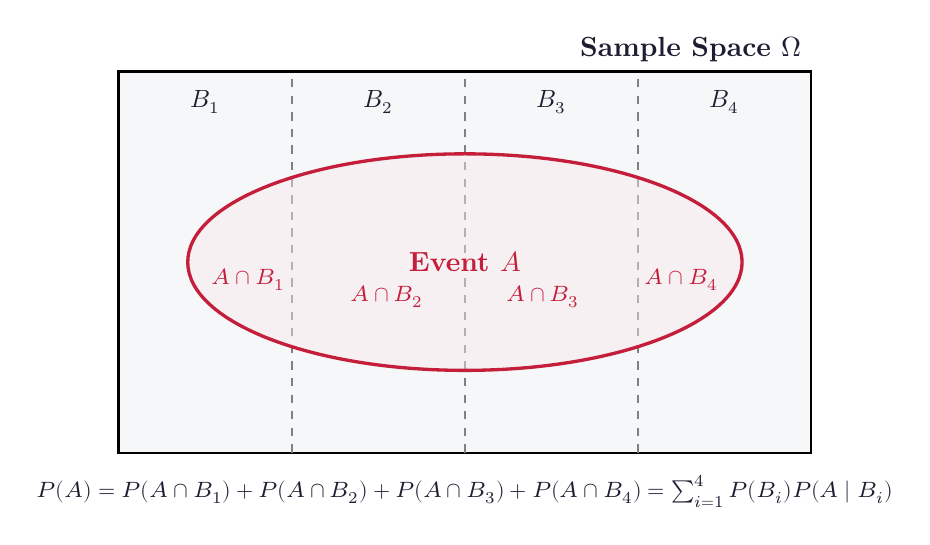
\begin{tikzpicture}[scale=1.1, every node/.style={font=\small}]
  % Sample space Omega rectangle
  \draw[thick, fill=mygray] (-4, -2.2) rectangle (4, 2.2);
  \node[above left, color=mydark, font=\bfseries] at (4, 2.2) {Sample Space $\Omega$};

  % Partition vertical dashed lines
  \draw[thick, dashed, color=gray] (-2, -2.2) -- (-2, 2.2);
  \draw[thick, dashed, color=gray] (0, -2.2) -- (0, 2.2);
  \draw[thick, dashed, color=gray] (2, -2.2) -- (2, 2.2);

  % Partition labels
  \node[above, color=mydark] at (-3, 1.6) {$B_1$};
  \node[above, color=mydark] at (-1, 1.6) {$B_2$};
  \node[above, color=mydark] at (1, 1.6) {$B_3$};
  \node[above, color=mydark] at (3, 1.6) {$B_4$};

  % Event A ellipse intersecting all partitions
  \draw[very thick, color=myred, fill=hdrred, fill opacity=0.45] (0, 0) ellipse (3.2cm and 1.25cm);
  \node[color=myred, font=\bfseries] at (0, 0) {Event $A$};

  % Slices of A in each partition
  \node[color=myred, font=\footnotesize] at (-2.5, -0.2) {$A \cap B_1$};
  \node[color=myred, font=\footnotesize] at (-0.9, -0.4) {$A \cap B_2$};
  \node[color=myred, font=\footnotesize] at (0.9, -0.4) {$A \cap B_3$};
  \node[color=myred, font=\footnotesize] at (2.5, -0.2) {$A \cap B_4$};

  % Caption
  \node[below, color=mydark, font=\footnotesize] at (0, -2.35) {
    $P(A) = P(A \cap B_1) + P(A \cap B_2) + P(A \cap B_3) + P(A \cap B_4) = \sum_{i=1}^4 P(B_i) P(A \mid B_i)$
  };
\end{tikzpicture}
\end{center}
\end{tcolorbox}

% ───────────────────────────────────────────────────────────────────────────────
\section{Discrete Random Variables, PMF and CDF}
% ───────────────────────────────────────────────────────────────────────────────

\begin{tcolorbox}[defbox, title={\textbf{Definition: Discrete Random Variable}}]
A \textbf{random variable (RV)} $X$ is a real-valued measurable function mapping the sample space into the real line:
\begin{equation}
  X: \Omega \longrightarrow \mathbb{R}
\end{equation}
A random variable is called \textbf{discrete} if its range $R_X = X(\Omega)$ is a finite or countably infinite set $\{x_1, x_2, x_3, \dots\}$.
\end{tcolorbox}

\subsection{Probability Mass Function (PMF)}
The \textbf{Probability Mass Function (PMF)} assigns probabilities directly to individual realization values $x_i$:
\begin{equation}
  p_X(x_i) = P(X = x_i) = P(\{\omega \in \Omega : X(\omega) = x_i\})
\end{equation}
Every valid discrete PMF must satisfy two fundamental conditions:
\begin{enumerate}[leftmargin=*, itemsep=2pt]
  \item \textbf{Non-negativity:} $p_X(x_i) \ge 0 \quad \forall x_i \in R_X$
  \item \textbf{Unit Normalization:} $\sum_{i} p_X(x_i) = 1$
\end{enumerate}

\subsection{Cumulative Distribution Function (CDF)}
The \textbf{Cumulative Distribution Function (CDF)}, denoted by $F_X(x)$, defines the probability that the random variable $X$ takes on a value less than or equal to a specified threshold $x \in \mathbb{R}$:
\begin{equation}
  F_X(x) = P(X \le x) = \sum_{x_i \le x} p_X(x_i)
\end{equation}

\begin{tcolorbox}[formulabox, title={\textbf{Mathematical Properties of the Discrete CDF}}]
The CDF $F_X(x)$ of any discrete random variable satisfies:
\begin{enumerate}[leftmargin=*, itemsep=3pt]
  \item \textbf{Boundary Limits:} $\displaystyle\lim_{x \to -\infty} F_X(x) = 0 \quad \text{and} \quad \lim_{x \to +\infty} F_X(x) = 1$
  \item \textbf{Monotonic Non-Decreasing:} If $a < b$, then $F_X(a) \le F_X(b)$.
  \item \textbf{Right-Continuity:} $\displaystyle\lim_{h \to 0^+} F_X(x + h) = F_X(x)$
  \item \textbf{Step Discontinuities (Jump Heights):} At every point $x_k$ with non-zero mass $p_X(x_k) > 0$, $F_X(x)$ exhibits a jump discontinuity of magnitude equal to the PMF:
  \begin{equation}
    P(X = x_k) = F_X(x_k) - F_X(x_k^-) = F_X(x_k) - \lim_{\epsilon \to 0^+} F_X(x_k - \epsilon)
  \end{equation}
  \item \textbf{Interval Probabilities:}
  \begin{align}
    P(a < X \le b) &= F_X(b) - F_X(a) \\[2pt]
    P(a \le X \le b) &= F_X(b) - F_X(a^-) = F_X(b) - F_X(a) + P(X = a)
  \end{align}
\end{enumerate}
\end{tcolorbox}

\begin{tcolorbox}[tikzbox, title={\textbf{TikZ Illustration: Discrete PMF Stems and Corresponding Staircase CDF}}]
\begin{center}
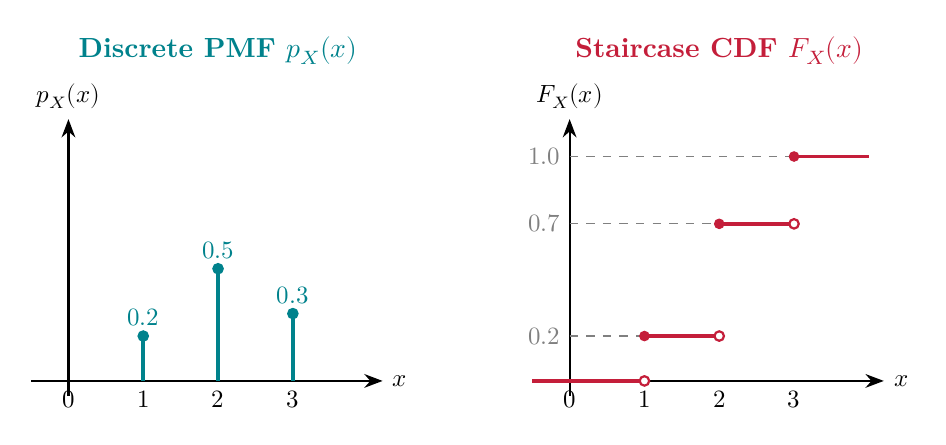
\begin{tikzpicture}[scale=0.95, every node/.style={font=\small}]
  % Left side: PMF
  \begin{scope}[shift={(-4.2,0)}]
    \draw[-Stealth, thick] (-0.5,0) -- (4.2,0) node[right] {$x$};
    \draw[-Stealth, thick] (0,-0.2) -- (0,3.5) node[above] {$p_X(x)$};

    % Stems
    \draw[line width=1.5pt, color=myteal] (1,0) -- (1,0.6);
    \filldraw[color=myteal] (1,0.6) circle (2pt) node[above] {$0.2$};
    \node[below] at (1,0) {$1$};

    \draw[line width=1.5pt, color=myteal] (2,0) -- (2,1.5);
    \filldraw[color=myteal] (2,1.5) circle (2pt) node[above] {$0.5$};
    \node[below] at (2,0) {$2$};

    \draw[line width=1.5pt, color=myteal] (3,0) -- (3,0.9);
    \filldraw[color=myteal] (3,0.9) circle (2pt) node[above] {$0.3$};
    \node[below] at (3,0) {$3$};

    \node[below] at (0,0) {$0$};
    \node[above, color=myteal, font=\bfseries] at (2.0, 4.1) {Discrete PMF $p_X(x)$};
  \end{scope}

  % Right side: CDF Staircase
  \begin{scope}[shift={(2.5,0)}]
    \draw[-Stealth, thick] (-0.5,0) -- (4.2,0) node[right] {$x$};
    \draw[-Stealth, thick] (0,-0.2) -- (0,3.5) node[above] {$F_X(x)$};

    % Levels: 0 before x=1, 0.2 from 1 to 2, 0.7 from 2 to 3, 1.0 for x >= 3
    % y-axis ticks: 0.2 -> 0.6, 0.7 -> 2.1, 1.0 -> 3.0
    \draw[dashed, color=gray] (0, 0.6) node[left] {$0.2$} -- (1, 0.6);
    \draw[dashed, color=gray] (0, 2.1) node[left] {$0.7$} -- (2, 2.1);
    \draw[dashed, color=gray] (0, 3.0) node[left] {$1.0$} -- (3, 3.0);

    % Stair segments
    \draw[very thick, color=myred] (-0.5, 0) -- (1, 0);
    \draw[fill=white, draw=myred, thick] (1,0) circle (1.8pt);

    \draw[very thick, color=myred] (1, 0.6) -- (2, 0.6);
    \filldraw[color=myred] (1, 0.6) circle (1.8pt);
    \draw[fill=white, draw=myred, thick] (2, 0.6) circle (1.8pt);

    \draw[very thick, color=myred] (2, 2.1) -- (3, 2.1);
    \filldraw[color=myred] (2, 2.1) circle (1.8pt);
    \draw[fill=white, draw=myred, thick] (3, 2.1) circle (1.8pt);

    \draw[very thick, color=myred] (3, 3.0) -- (4.0, 3.0);
    \filldraw[color=myred] (3, 3.0) circle (1.8pt);

    % Ticks on x-axis
    \node[below] at (1,0) {$1$};
    \node[below] at (2,0) {$2$};
    \node[below] at (3,0) {$3$};
    \node[below] at (0,0) {$0$};

    \node[above, color=myred, font=\bfseries] at (2.0, 4.1) {Staircase CDF $F_X(x)$};
  \end{scope}
\end{tikzpicture}
\end{center}
\end{tcolorbox}

% ───────────────────────────────────────────────────────────────────────────────
\section{Expectation, Moments, Variance, Covariance and Correlation}
% ───────────────────────────────────────────────────────────────────────────────

\begin{tcolorbox}[defbox, title={\textbf{Definition: Mathematical Expectation of a Discrete RV}}]
Let $X$ be a discrete random variable with PMF $p_X(x)$. The \textbf{expected value} (or mathematical expectation / first raw moment) of $X$ is defined as:
\begin{equation}
  E[X] = \mu = \sum_{x \in R_X} x \cdot p_X(x)
\end{equation}
provided that the series converges absolutely: $\sum_{x} |x| p_X(x) < \infty$. If the series diverges, the expectation does not exist.
\end{tcolorbox}

\subsection{Properties of Mathematical Expectation}
For arbitrary constants $a, b \in \mathbb{R}$ and measurable functions $g(X), h(X)$:
\begin{enumerate}[leftmargin=*, itemsep=3pt]
  \item \textbf{Expectation of a Constant:} $E[c] = c \sum p_X(x) = c$.
  \item \textbf{Linearity of Expectation:} For any random variables $X$ and $Y$ (independent or dependent!):
  \begin{equation}
    E[aX + bY + c] = aE[X] + bE[Y] + c
  \end{equation}
  \item \textbf{Law of the Unconscious Statistician (LOTUS):} For any function $g(X)$:
  \begin{equation}
    E[g(X)] = \sum_{x \in R_X} g(x) \cdot p_X(x)
  \end{equation}
  \item \textbf{Product Rule for Independent RVs:} If $X$ and $Y$ are independent:
  \begin{equation}
    E[X \cdot Y] = E[X] \cdot E[Y]
  \end{equation}
\end{enumerate}

\subsection{Moments: Raw Moments and Central Moments}
\begin{itemize}[leftmargin=*, itemsep=3pt]
  \item \textbf{$r$-th Raw Moment ($\mu_r'$):} Expectation about the origin:
  \begin{equation}
    \mu_r' = E[X^r] = \sum_{x} x^r p_X(x), \quad \mu_1' = \mu = E[X]
  \end{equation}
  \item \textbf{$r$-th Central Moment ($\mu_r$):} Expectation about the mean $\mu$:
  \begin{equation}
    \mu_r = E[(X - \mu)^r] = \sum_{x} (x - \mu)^r p_X(x)
  \end{equation}
  Specifically:
  \begin{align}
    \mu_0 &= E[(X-\mu)^0] = 1 \\[2pt]
    \mu_1 &= E[X - \mu] = E[X] - \mu = 0 \quad (\text{Always zero!}) \\[2pt]
    \mu_2 &= E[(X - \mu)^2] = \operatorname{Var}(X) = \sigma^2 \\[2pt]
    \mu_3 &= E[(X - \mu)^3] = \mu_3' - 3\mu_2'\mu + 2\mu^3 \quad (\text{Skewness measure}) \\[2pt]
    \mu_4 &= E[(X - \mu)^4] = \mu_4' - 4\mu_3'\mu + 6\mu_2'\mu^2 - 3\mu^4 \quad (\text{Kurtosis measure})
  \end{align}
\end{itemize}

\begin{tcolorbox}[formulabox, title={\textbf{Variance and Standard Deviation}}]
The \textbf{variance} of $X$, denoted $\operatorname{Var}(X)$ or $\sigma^2$, measures the degree of dispersion around the mean:
\begin{equation}
  \operatorname{Var}(X) = \sigma^2 = E\left[(X - E[X])^2\right] = E[X^2] - (E[X])^2 = \mu_2' - (\mu_1')^2
\end{equation}
\textbf{Fundamental Properties of Variance:}
\begin{enumerate}[leftmargin=*, itemsep=2pt]
  \item $\operatorname{Var}(X) \ge 0$, and $\operatorname{Var}(X) = 0 \iff X = c$ (constant with probability 1).
  \item $\operatorname{Var}(aX + b) = a^2 \operatorname{Var}(X)$. Adding a constant shifts position without altering spread!
  \item Standard deviation is $\sigma = \sqrt{\operatorname{Var}(X)}$, which retains the original units of $X$.
\end{enumerate}
\end{tcolorbox}

\begin{tcolorbox}[defbox, title={\textbf{Definition: Covariance and Correlation Coefficient}}]
\textbf{Covariance:} For two random variables $X$ and $Y$ with means $\mu_X$ and $\mu_Y$, their \textbf{covariance} is:
\begin{equation}
  \operatorname{Cov}(X, Y) = \sigma_{XY} = E[(X - \mu_X)(Y - \mu_Y)] = E[XY] - \mu_X \mu_Y
\end{equation}
\textbf{Pearson Correlation Coefficient ($\rho$):} Normalized measure of linear dependence:
\begin{equation}
  \rho(X, Y) = \frac{\operatorname{Cov}(X, Y)}{\sigma_X \sigma_Y} = \frac{E[XY] - E[X]E[Y]}{\sqrt{\operatorname{Var}(X)\operatorname{Var}(Y)}}
\end{equation}
\end{tcolorbox}

\subsection{Proof that \texorpdfstring{$-1 \le \rho \le 1$}{-1 <= rho <= 1}}
\begin{tcolorbox}[examplebox, title={\textbf{Rigorous Derivation: Cauchy-Schwarz Bound on Correlation}}]
Consider the standardized variables $U = \frac{X - \mu_X}{\sigma_X}$ and $V = \frac{Y - \mu_Y}{\sigma_Y}$. Clearly $E[U] = E[V] = 0$, $E[U^2] = E[V^2] = 1$, and $E[UV] = \rho$.
For any real scalar $t \in \mathbb{R}$, define the quadratic form:
\begin{equation}
  Q(t) = E\left[(t U + V)^2\right] \ge 0 \quad (\text{since the square of a real quantity is non-negative})
\end{equation}
Expanding the quadratic expectation:
\begin{align}
  Q(t) &= E\left[t^2 U^2 + 2t UV + V^2\right] \nonumber \\
       &= t^2 E[U^2] + 2t E[UV] + E[V^2] \nonumber \\
       &= t^2 (1) + 2t \rho + 1 \ge 0 \quad \forall t \in \mathbb{R}
\end{align}
For a quadratic $A t^2 + B t + C \ge 0$ with $A = 1 > 0$ to remain non-negative for all real $t$, its discriminant $\Delta = B^2 - 4AC$ must be non-positive:
\begin{equation}
  \Delta = (2\rho)^2 - 4(1)(1) \le 0 \implies 4\rho^2 - 4 \le 0 \implies \rho^2 \le 1
\end{equation}
Taking square roots yields:
\begin{equation}
  -1 \le \rho \le 1
\end{equation}
\begin{itemize}[leftmargin=*, itemsep=1pt]
  \item $\rho = +1$: Perfect positive linear relationship ($Y = aX + b$ with $a > 0$).
  \item $\rho = -1$: Perfect negative linear relationship ($Y = aX + b$ with $a < 0$).
  \item $\rho = 0$: $X$ and $Y$ are \textbf{uncorrelated}. Note: Independent $\implies$ Uncorrelated, but Uncorrelated does not imply Independent!
\end{itemize}
\end{tcolorbox}

\subsection{Variance of a Sum of Random Variables}
For $n$ random variables $X_1, X_2, \dots, X_n$:
\begin{equation}
  \operatorname{Var}\left(\sum_{i=1}^n X_i\right) = \sum_{i=1}^n \operatorname{Var}(X_i) + 2 \sum_{1 \le i < j \le n} \operatorname{Cov}(X_i, X_j)
\end{equation}
For two variables:
\begin{equation}
  \operatorname{Var}(aX \pm bY) = a^2 \operatorname{Var}(X) + b^2 \operatorname{Var}(Y) \pm 2ab \operatorname{Cov}(X, Y)
\end{equation}
If $X$ and $Y$ are independent (or merely uncorrelated so that $\operatorname{Cov}(X,Y) = 0$):
\begin{equation}
  \operatorname{Var}(X + Y) = \operatorname{Var}(X - Y) = \operatorname{Var}(X) + \operatorname{Var}(Y)
\end{equation}

% ───────────────────────────────────────────────────────────────────────────────
\section{Bernoulli Trials, Multinomial, Poisson Approximation \& Convolutions}
% ───────────────────────────────────────────────────────────────────────────────

\subsection{Bernoulli Trials and Binomial Distribution}
A \textbf{Bernoulli trial} is an experiment with exactly two mutually exclusive outcomes: \textit{Success} ($S$) with probability $p$, and \textit{Failure} ($F$) with probability $q = 1 - p$.
In a sequence of $n$ independent and identical Bernoulli trials:
\begin{tcolorbox}[formulabox, title={\textbf{Binomial Distribution $\mathbf{Bin(n, p)}$}}]
The random variable $X$, representing the total number of successes in $n$ trials, follows the Binomial distribution:
\begin{equation}
  P(X = k) = \binom{n}{k} p^k q^{n-k} = \frac{n!}{k!(n-k)!} p^k (1-p)^{n-k}, \quad k \in \{0, 1, 2, \dots, n\}
\end{equation}
Statistical parameters:
\begin{equation}
  E[X] = np, \qquad \operatorname{Var}(X) = npq = np(1-p), \qquad \sigma_X = \sqrt{np(1-p)}
\end{equation}
Since $q = 1-p < 1$, the variance of a Binomial distribution is strictly less than its mean: $\operatorname{Var}(X) < E[X]$.
\end{tcolorbox}

\subsection{Multinomial Distribution}
The \textbf{Multinomial distribution} generalizes the Binomial distribution to trials having $k \ge 2$ mutually exclusive outcomes $E_1, E_2, \dots, E_k$ with respective constant probabilities $p_1, p_2, \dots, p_k$ where $\sum_{j=1}^k p_j = 1$.
\begin{tcolorbox}[defbox, title={\textbf{Definition: Multinomial PMF}}]
In $n$ independent repetitions, let $X_j$ denote the number of times event $E_j$ occurs ($\sum_{j=1}^k X_j = n$). The joint PMF is:
\begin{equation}
  P(X_1 = x_1, X_2 = x_2, \dots, X_k = x_k) = \frac{n!}{x_1! x_2! \cdots x_k!} p_1^{x_1} p_2^{x_2} \cdots p_k^{x_k}
\end{equation}
where $x_j \in \{0, 1, \dots, n\}$ and $\sum_{j=1}^k x_j = n$.
\textbf{Moments and Covariances:}
\begin{equation}
  E[X_j] = n p_j, \qquad \operatorname{Var}(X_j) = n p_j (1 - p_j), \qquad \operatorname{Cov}(X_i, X_j) = -n p_i p_j \quad (i \ne j)
\end{equation}
\textit{Key Insight:} Covariance is strictly negative because an increase in occurrences of event $E_i$ constrains the remaining trials available for event $E_j$.
\end{tcolorbox}

\subsection{Poisson Approximation to the Binomial Distribution (Law of Rare Events)}
When the number of trials $n$ is very large ($n \to \infty$) and the success probability $p$ is very small ($p \to 0$) such that the average occurrence rate $\lambda = np$ remains a finite positive constant:
\begin{tcolorbox}[examplebox, title={\textbf{Rigorous Derivation: Poisson Limit Theorem}}]
Starting from the Binomial PMF:
\begin{equation}
  P(X = k) = \binom{n}{k} p^k (1-p)^{n-k} = \frac{n(n-1)(n-2)\cdots(n-k+1)}{k!} \left(\frac{\lambda}{n}\right)^k \left(1 - \frac{\lambda}{n}\right)^{n-k}
\end{equation}
Rearranging terms:
\begin{equation}
  P(X = k) = \frac{\lambda^k}{k!} \cdot \left[\frac{n}{n} \cdot \frac{n-1}{n} \cdot \frac{n-2}{n} \cdots \frac{n-k+1}{n}\right] \cdot \left(1 - \frac{\lambda}{n}\right)^n \cdot \left(1 - \frac{\lambda}{n}\right)^{-k}
\end{equation}
Taking the limit as $n \to \infty$ for fixed $k$:
\begin{align}
  \lim_{n \to \infty} \left(1 - \frac{1}{n}\right)\left(1 - \frac{2}{n}\right)\cdots\left(1 - \frac{k-1}{n}\right) &= 1 \cdot 1 \cdots 1 = 1 \\[3pt]
  \lim_{n \to \infty} \left(1 - \frac{\lambda}{n}\right)^n &= e^{-\lambda} \\[3pt]
  \lim_{n \to \infty} \left(1 - \frac{\lambda}{n}\right)^{-k} &= (1 - 0)^{-k} = 1
\end{align}
Multiplying these limits:
\begin{equation}
  \lim_{n \to \infty} P(X = k) = \frac{\lambda^k e^{-\lambda}}{k!}, \qquad k = 0, 1, 2, \dots
\end{equation}
This is the PMF of the \textbf{Poisson distribution} with parameter $\lambda = np$. For Poisson, $E[X] = \operatorname{Var}(X) = \lambda$.
\end{tcolorbox}

\begin{tcolorbox}[tikzbox, title={\textbf{TikZ Plot: Binomial PMF ($n=20, p=0.1$) vs. Poisson PMF ($\lambda = np = 2.0$)}}]
\begin{center}
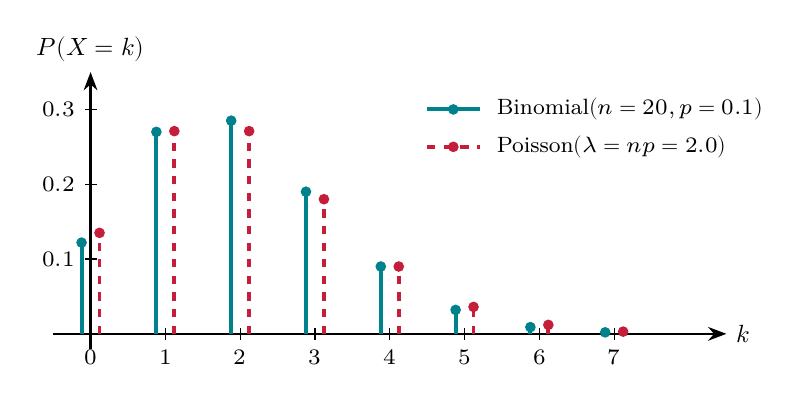
\begin{tikzpicture}[scale=0.95, every node/.style={font=\small}]
  % Axes
  \draw[-Stealth, thick] (-0.5, 0) -- (8.5, 0) node[right] {$k$};
  \draw[-Stealth, thick] (0, -0.2) -- (0, 3.5) node[above] {$P(X=k)$};

  % Ticks on x-axis
  \foreach \x in {0,1,2,3,4,5,6,7} {
    \draw (\x, 0.08) -- (\x, -0.08) node[below] {\footnotesize $\x$};
  }

  % Ticks on y-axis (scale: prob 0.3 -> y=3.0)
  \draw (0.08, 1.0) -- (-0.08, 1.0) node[left] {\footnotesize $0.1$};
  \draw (0.08, 2.0) -- (-0.08, 2.0) node[left] {\footnotesize $0.2$};
  \draw (0.08, 3.0) -- (-0.08, 3.0) node[left] {\footnotesize $0.3$};

  % Data: (k, Binomial P, Poisson P)
  % k=0: Bin=0.1216 (1.22), Poi=0.1353 (1.35)
  % k=1: Bin=0.2702 (2.70), Poi=0.2707 (2.71)
  % k=2: Bin=0.2852 (2.85), Poi=0.2707 (2.71)
  % k=3: Bin=0.1901 (1.90), Poi=0.1804 (1.80)
  % k=4: Bin=0.0898 (0.90), Poi=0.0902 (0.90)
  % k=5: Bin=0.0319 (0.32), Poi=0.0361 (0.36)
  % k=6: Bin=0.0089 (0.09), Poi=0.0120 (0.12)
  % k=7: Bin=0.0020 (0.02), Poi=0.0034 (0.03)

  % Binomial stems (blue/teal, offset -0.1)
  \foreach \k/\h in {0/1.22, 1/2.70, 2/2.85, 3/1.90, 4/0.90, 5/0.32, 6/0.09, 7/0.02} {
    \draw[line width=1.4pt, color=myteal] ({\k-0.12}, 0) -- ({\k-0.12}, \h);
    \filldraw[color=myteal] ({\k-0.12}, \h) circle (1.8pt);
  }

  % Poisson stems (red/dashed, offset +0.1)
  \foreach \k/\h in {0/1.35, 1/2.71, 2/2.71, 3/1.80, 4/0.90, 5/0.36, 6/0.12, 7/0.03} {
    \draw[line width=1.4pt, color=myred, dashed] ({\k+0.12}, 0) -- ({\k+0.12}, \h);
    \filldraw[color=myred] ({\k+0.12}, \h) circle (1.8pt);
  }

  % Legend
  \draw[line width=1.4pt, color=myteal] (4.5, 3.0) -- (5.2, 3.0);
  \filldraw[color=myteal] (4.85, 3.0) circle (1.8pt);
  \node[right, font=\footnotesize] at (5.3, 3.0) {$\text{Binomial}(n=20, p=0.1)$};

  \draw[line width=1.4pt, color=myred, dashed] (4.5, 2.5) -- (5.2, 2.5);
  \filldraw[color=myred] (4.85, 2.5) circle (1.8pt);
  \node[right, font=\footnotesize] at (5.3, 2.5) {$\text{Poisson}(\lambda = np = 2.0)$};
\end{tikzpicture}
\end{center}
\end{tcolorbox}

\subsection{Infinite Sequences of Bernoulli Trials: Geometric Distribution}
When independent Bernoulli trials are repeated indefinitely until the \textbf{first success} occurs:
\begin{equation}
  P(X = k) = (1-p)^{k-1} p = q^{k-1} p, \qquad k \in \{1, 2, 3, \dots\}
\end{equation}
Properties of the \textbf{Geometric distribution}:
\begin{equation}
  E[X] = \frac{1}{p}, \qquad \operatorname{Var}(X) = \frac{1-p}{p^2} = \frac{q}{p^2}
\end{equation}
\textbf{Memoryless Property:} The geometric distribution is the \textit{only} discrete distribution possessing memorylessness:
\begin{equation}
  P(X > s + t \mid X > s) = P(X > t) \quad \forall s, t \in \mathbb{N}
\end{equation}

\subsection{Sums of Independent Random Variables (Discrete Convolution)}
Let $X$ and $Y$ be independent discrete integer-valued random variables with PMFs $p_X(x)$ and $p_Y(y)$. The PMF of their sum $Z = X + Y$ is obtained via \textbf{discrete convolution}:
\begin{equation}
  p_Z(z) = P(Z = z) = \sum_{k=-\infty}^\infty P(X = k, Y = z - k) = \sum_{k=-\infty}^\infty p_X(k) \cdot p_Y(z - k) = (p_X * p_Y)(z)
\end{equation}
\begin{tcolorbox}[formulabox, title={\textbf{Reproductive (Convolution) Properties of Key Discrete Distributions}}]
\begin{enumerate}[leftmargin=*, itemsep=3pt]
  \item \textbf{Sum of Independent Binomials:} If $X \sim \text{Bin}(n_1, p)$ and $Y \sim \text{Bin}(n_2, p)$ share the same success parameter $p$:
  \begin{equation}
    Z = X + Y \sim \text{Bin}(n_1 + n_2, p)
  \end{equation}
  \item \textbf{Sum of Independent Poissons:} If $X \sim \text{Poisson}(\lambda_1)$ and $Y \sim \text{Poisson}(\lambda_2)$:
  \begin{equation}
    Z = X + Y \sim \text{Poisson}(\lambda_1 + \lambda_2)
  \end{equation}
  \textit{Proof Sketch:} Using the convolution formula:
  \begin{equation}
    P(Z = z) = \sum_{k=0}^z \frac{e^{-\lambda_1} \lambda_1^k}{k!} \cdot \frac{e^{-\lambda_2} \lambda_2^{z-k}}{(z-k)!} = \frac{e^{-(\lambda_1+\lambda_2)}}{z!} \sum_{k=0}^z \binom{z}{k} \lambda_1^k \lambda_2^{z-k} = \frac{e^{-(\lambda_1+\lambda_2)} (\lambda_1+\lambda_2)^z}{z!}
  \end{equation}
\end{enumerate}
\end{tcolorbox}

% ───────────────────────────────────────────────────────────────────────────────
\section{Chebyshev's Inequality and Concentration Bounds}
% ───────────────────────────────────────────────────────────────────────────────

When the exact probability distribution of a random variable is unknown, Chebyshev's Inequality provides a guaranteed mathematical upper bound on the probability of significant deviations from the mean, requiring knowledge of only the mean $\mu$ and finite variance $\sigma^2$.

\begin{tcolorbox}[defbox, title={\textbf{Markov's Inequality (Foundation for Chebyshev)}}]
If $Y$ is a non-negative random variable ($P(Y \ge 0) = 1$) with finite expectation $E[Y] < \infty$, then for any positive real constant $a > 0$:
\begin{equation}
  P(Y \ge a) \le \frac{E[Y]}{a}
\end{equation}
\textbf{Proof:}
\begin{equation}
  E[Y] = \sum_{y} y p_Y(y) = \sum_{y < a} y p_Y(y) + \sum_{y \ge a} y p_Y(y) \ge \sum_{y \ge a} y p_Y(y) \ge a \sum_{y \ge a} p_Y(y) = a P(Y \ge a)
\end{equation}
Dividing both sides by $a > 0$ completes the proof.
\end{tcolorbox}

\begin{tcolorbox}[examplebox, title={\textbf{Rigorous Derivation of Chebyshev's Inequality}}]
Let $X$ be any random variable with mean $\mu = E[X]$ and variance $\sigma^2 = \operatorname{Var}(X) < \infty$.
Define the non-negative random variable $Y = (X - \mu)^2 \ge 0$.
Applying Markov's inequality to $Y$ with threshold $a = \epsilon^2$ (where $\epsilon > 0$):
\begin{equation}
  P\left(Y \ge \epsilon^2\right) \le \frac{E[Y]}{\epsilon^2} \implies P\left((X - \mu)^2 \ge \epsilon^2\right) \le \frac{E\left[(X - \mu)^2\right]}{\epsilon^2}
\end{equation}
Since $(X - \mu)^2 \ge \epsilon^2 \iff |X - \mu| \ge \epsilon$, and $E[(X - \mu)^2] = \sigma^2$:
\begin{equation}
  P(|X - \mu| \ge \epsilon) \le \frac{\sigma^2}{\epsilon^2}
\end{equation}
Substituting $\epsilon = k\sigma$ (where $k > 0$ represents the deviation in units of standard deviations):
\begin{equation}
  P(|X - \mu| \ge k\sigma) \le \frac{1}{k^2}
\end{equation}
Taking the complementary event yields the dual form:
\begin{equation}
  P(|X - \mu| < k\sigma) \ge 1 - \frac{1}{k^2}
\end{equation}
\end{tcolorbox}

\begin{tcolorbox}[tikzbox, title={\textbf{TikZ Schematic: Geometric Interpretation of Chebyshev's Concentration Bound}}]
\begin{center}
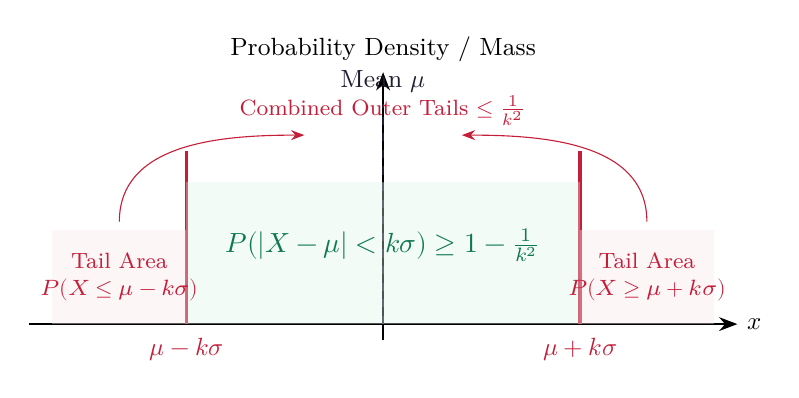
\begin{tikzpicture}[scale=1.0, every node/.style={font=\small}]
  % Axis
  \draw[-Stealth, thick] (-4.5, 0) -- (4.5, 0) node[right] {$x$};
  \draw[-Stealth, thick] (0, -0.2) -- (0, 3.2) node[above] {Probability Density / Mass};

  % Mean center line
  \draw[thick, dashed, color=mydark] (0, 0) -- (0, 2.8) node[above] {Mean $\mu$};

  % Symmetric bounds: mu - k*sigma and mu + k*sigma
  \draw[very thick, color=myred] (-2.5, 0) -- (-2.5, 2.2);
  \node[below, color=myred] at (-2.5, -0.05) {$\mu - k\sigma$};

  \draw[very thick, color=myred] (2.5, 0) -- (2.5, 2.2);
  \node[below, color=myred] at (2.5, -0.05) {$\mu + k\sigma$};

  % Shaded central interval
  \fill[fill=hdrgreen, fill opacity=0.35] (-2.5, 0) rectangle (2.5, 1.8);
  \node[color=mygreen, font=\bfseries] at (0, 1.0) {$P(|X - \mu| < k\sigma) \ge 1 - \frac{1}{k^2}$};

  % Shaded outer tails
  \fill[fill=hdrred, fill opacity=0.4] (-4.2, 0) rectangle (-2.5, 1.2);
  \fill[fill=hdrred, fill opacity=0.4] (2.5, 0) rectangle (4.2, 1.2);
  \node[color=myred, font=\footnotesize, align=center] at (-3.35, 0.6) {Tail Area\\$P(X \le \mu - k\sigma)$};
  \node[color=myred, font=\footnotesize, align=center] at (3.35, 0.6) {Tail Area\\$P(X \ge \mu + k\sigma)$};

  % Total tail bound note
  \draw[-Stealth, thin, color=myred] (-3.35, 1.3) to[out=90, in=180] (-1.0, 2.4);
  \draw[-Stealth, thin, color=myred] (3.35, 1.3) to[out=90, in=0] (1.0, 2.4);
  \node[above, color=myred, font=\footnotesize] at (0, 2.4) {Combined Outer Tails $\le \frac{1}{k^2}$};
\end{tikzpicture}
\end{center}
\end{tcolorbox}

\subsection{Numerical Significance of Chebyshev's Bound}
\par\vspace{6pt}\noindent
\begingroup
\setlength{\tabcolsep}{6pt}
\setlength{\extrarowheight}{3pt}
\begin{tabularx}{\linewidth}{|B{2.2cm}|B{3.8cm}|B{4.0cm}|Y|}
\hline
\textbf{Spread ($k$)} & \textbf{Interval $[\mu - k\sigma, \mu + k\sigma]$} & \textbf{Chebyshev Bound ($P \ge 1 - 1/k^2$)} & \textbf{Normal Distribution Comparison} \\
\hline
$k = 1$ & $[\mu - \sigma, \mu + \sigma]$ & $\ge 0\%$ (Trivial bound) & $\approx 68.27\%$ \\
\hline
$k = 2$ & $[\mu - 2\sigma, \mu + 2\sigma]$ & $\ge 1 - 1/4 = 75.00\%$ & $\approx 95.45\%$ \\
\hline
$k = 3$ & $[\mu - 3\sigma, \mu + 3\sigma]$ & $\ge 1 - 1/9 = 88.89\%$ & $\approx 99.73\%$ \\
\hline
$k = 4$ & $[\mu - 4\sigma, \mu + 4\sigma]$ & $\ge 1 - 1/16 = 93.75\%$ & $\approx 99.9937\%$ \\
\hline
\end{tabularx}
\endgroup
\vspace{12pt}

\newpage
% ===============================================================================
% MANDATORY QUICK REVISION PAGE
% ===============================================================================
\begin{center}
  {\large\bfseries\color{myred} Quick Revision --- Module 1}\\[2pt]
  {\small\color{mydark} Basic Probability, Discrete Random Variables and Inequalities $|$ BS-M301}
\end{center}
\noindent{\color{myred}\rule{\linewidth}{1.0pt}}
\vspace{2pt}

\begin{tcolorbox}[formulabox, top=3pt, bottom=3pt, title={\textbf{Key Formulas and Probability Identities at a Glance}}]
\renewcommand{\arraystretch}{1.10}
\begin{tabularx}{\linewidth}{B{4.8cm} X}
Kolmogorov Axioms & $P(A) \ge 0, \quad P(\Omega) = 1, \quad P\left(\bigcup_{i=1}^\infty A_i\right) = \sum_{i=1}^\infty P(A_i) \text{ (disjoint)}$ \\[1pt]
Addition Law & $P(A \cup B) = P(A) + P(B) - P(A \cap B)$ \\[1pt]
Conditional Probability & $P(A \mid B) = \frac{P(A \cap B)}{P(B)}, \quad P(A \cap B) = P(A) \cdot P(B) \text{ (Independence)}$ \\[1pt]
Total Probability & $P(A) = \sum_{i=1}^n P(B_i) P(A \mid B_i) \quad (\text{Partition } \{B_i\})$ \\[1pt]
Bayes' Theorem & $P(B_k \mid A) = \frac{P(B_k) P(A \mid B_k)}{\sum_{i=1}^n P(B_i) P(A \mid B_i)}$ \\[1pt]
Discrete Expectation & $E[X] = \mu = \sum_x x p_X(x), \quad E[aX + bY] = aE[X] + bE[Y]$ \\[1pt]
Variance Formula & $\operatorname{Var}(X) = \sigma^2 = E[X^2] - (E[X])^2, \quad \operatorname{Var}(aX+b) = a^2 \operatorname{Var}(X)$ \\[1pt]
Covariance \& Correlation & $\operatorname{Cov}(X,Y) = E[XY] - \mu_X \mu_Y, \quad \rho = \frac{\operatorname{Cov}(X,Y)}{\sigma_X \sigma_Y} \in [-1, 1]$ \\[1pt]
Binomial Distribution & $P(X=k) = \binom{n}{k} p^k q^{n-k}, \quad \mu = np, \; \sigma^2 = npq$ \\[1pt]
Poisson Approximation & $P(X=k) = \frac{\lambda^k e^{-\lambda}}{k!}, \quad \lambda = np, \; \mu = \sigma^2 = \lambda$ \\[1pt]
Chebyshev's Inequality & $P(|X - \mu| \ge k\sigma) \le \frac{1}{k^2}, \quad P(|X - \mu| < k\sigma) \ge 1 - \frac{1}{k^2}$ \\
\end{tabularx}
\end{tcolorbox}

\vspace{1pt}

\begin{tcolorbox}[defbox, top=3pt, bottom=3pt, title={\textbf{One-Line Definitions}}]
\begin{itemize}[leftmargin=*, itemsep=0.5pt, topsep=0pt]
  \item \textbf{Probability Space $(\Omega, \mathcal{F}, P)$:} Formal triplet of sample space, $\sigma$-algebra of events, and Kolmogorov measure.
  \item \textbf{$\sigma$-algebra ($\mathcal{F}$):} Event collection closed under complementation and countable unions containing $\Omega$.
  \item \textbf{Statistical Independence:} Condition where $P(A \cap B) = P(A)P(B)$, giving zero mutual information.
  \item \textbf{Random Variable:} A measurable real-valued function $X: \Omega \to \mathbb{R}$ mapping outcomes to real numbers.
  \item \textbf{Probability Mass Function (PMF):} Discrete assignment $p_X(x) = P(X=x)$ with non-negativity and unit sum.
  \item \textbf{Cumulative Distribution Function (CDF):} Non-decreasing right-continuous probability $F_X(x) = P(X \le x)$.
  \item \textbf{Law of Rare Events:} Poisson convergence of Binomial distribution when $n \to \infty, p \to 0$ with $\lambda = np$ constant.
  \item \textbf{Memoryless Property:} Invariance condition $P(X > s+t \mid X > s) = P(X > t)$, uniquely held by Geometric distribution.
  \item \textbf{Uncorrelated Variables:} Variables with zero covariance ($\operatorname{Cov}(X,Y) = 0, \rho = 0$), weaker than full independence.
  \item \textbf{Chebyshev's Bound:} Non-parametric inequality guaranteeing at least $(1 - 1/k^2)$ probability mass within $\mu \pm k\sigma$.
\end{itemize}
\end{tcolorbox}

\newpage

\begin{tcolorbox}[exambox, title={\textbf{Frequently Asked / Viva Questions (Part 1)}}]
\begin{enumerate}[topsep=0pt, label=\textbf{Q\arabic*.}, itemsep=3.2pt]
  \item \Q{State Kolmogorov's Axioms of Probability and derive $P(\emptyset) = 0$.}
  Axiom 1: $P(A) \ge 0$. Axiom 2: $P(\Omega) = 1$. Axiom 3: Countable additivity for pairwise disjoint events. Since $\Omega = \Omega \cup \emptyset$ with $\Omega \cap \emptyset = \emptyset$, Axiom 3 yields $P(\Omega) = P(\Omega) + P(\emptyset) \implies P(\emptyset) = 0$.

  \item \Q{Distinguish between pairwise independence and mutual independence with an example.}
  Pairwise independence requires $P(A_i \cap A_j) = P(A_i)P(A_j)$ for all pairs. Mutual independence additionally requires the product rule across all $k$-tuples up to all $n$ events. In Bernstein's example (tossing two coins, $A$: heads on coin 1, $B$: heads on coin 2, $C$: both same), events are pairwise independent but not mutually independent.

  \item \Q{State and prove the Law of Total Probability.}
  If $\{B_1, \dots, B_n\}$ partitions $\Omega$, then $A = A \cap \Omega = \bigcup_{i=1}^n (A \cap B_i)$. Because the partitions are disjoint, the slices $(A \cap B_i)$ are mutually exclusive. By additivity, $P(A) = \sum_{i=1}^n P(A \cap B_i) = \sum_{i=1}^n P(B_i) P(A \mid B_i)$.

  \item \Q{Under what physical conditions does the Binomial distribution tend to the Poisson distribution?}
  When the number of independent trials $n \to \infty$, the probability of success on each trial $p \to 0$, such that the expected average number of occurrences $\lambda = np$ remains a finite positive constant (the law of rare events).

  \item \Q{Prove that for any random variable with finite variance, $\operatorname{Var}(aX + b) = a^2 \operatorname{Var}(X)$.}
  $E[aX + b] = a\mu + b$. Then $\operatorname{Var}(aX + b) = E[((aX + b) - (a\mu + b))^2] = E[(a(X - \mu))^2] = E[a^2 (X - \mu)^2] = a^2 E[(X - \mu)^2] = a^2 \operatorname{Var}(X)$. Adding a constant shifts the distribution without affecting spread.

  \item \Q{Why is covariance negative for components of a Multinomial distribution?}
  In a multinomial distribution, $\sum_{j=1}^k X_j = n$ is fixed. If event $i$ occurs more frequently ($X_i > E[X_i]$), fewer trials remain available for other events ($X_j < E[X_j]$), creating a deterministic negative association: $\operatorname{Cov}(X_i, X_j) = -n p_i p_j < 0$.

  \item \Q{Does zero correlation ($\rho = 0$) imply independence of two random variables?}
  No! Independence implies uncorrelatedness ($\operatorname{Cov}(X, Y) = 0 \implies \rho = 0$), but the converse is not true in general. For example, if $X \sim U[-1, 1]$ and $Y = X^2$, then $E[X] = 0$ and $E[XY] = E[X^3] = 0$, giving $\operatorname{Cov}(X, Y) = 0$ and $\rho = 0$, yet $Y$ is completely deterministically dependent on $X$!
\end{enumerate}
\end{tcolorbox}

\newpage

\begin{tcolorbox}[exambox, top=3pt, bottom=3pt, title={\textbf{Frequently Asked / Viva Questions (Part 2)}}]
\begin{enumerate}[topsep=0pt, label=\textbf{Q\arabic*.}, itemsep=1.8pt, start=8]
  \item \Q{State and prove Chebyshev's Inequality using Markov's Inequality.}
  Markov's inequality for non-negative $Y \ge 0$ states $P(Y \ge a) \le E[Y]/a$. Defining $Y = (X - \mu)^2 \ge 0$ and setting $a = k^2 \sigma^2$: $P((X - \mu)^2 \ge k^2 \sigma^2) \le E[(X - \mu)^2] / (k^2 \sigma^2) = \sigma^2 / (k^2 \sigma^2) = 1/k^2$. Since $(X - \mu)^2 \ge k^2 \sigma^2 \iff |X - \mu| \ge k\sigma$, we obtain $P(|X - \mu| \ge k\sigma) \le 1/k^2$.

  \item \Q{What is the reproductive property of independent Poisson random variables?}
  The sum of two independent Poisson variables $X \sim \text{Poisson}(\lambda_1)$ and $Y \sim \text{Poisson}(\lambda_2)$ is itself a Poisson random variable with parameter $\lambda_1 + \lambda_2$. This follows from the binomial expansion within the discrete convolution sum.

  \item \Q{Explain the memoryless property of the Geometric distribution.}
  $P(X > s + t \mid X > s) = P(X > t)$ for integers $s, t \ge 1$. If $s$ consecutive failures have already occurred, the probability of requiring at least $t$ additional trials until the first success is identical to the initial probability of requiring at least $t$ trials. The system has no memory of past failures.
\end{enumerate}
\end{tcolorbox}

\vspace{2pt}

\begin{tcolorbox}[tikzbox, top=3pt, bottom=3pt, title={\textbf{Summary Matrix: Comprehensive Comparison of Discrete Probability Distributions}}]
\par\vspace{1pt}\noindent
\begingroup
\setlength{\tabcolsep}{3.5pt}
\setlength{\extrarowheight}{1.0pt}
\renewcommand{\arraystretch}{1.12}
\begin{tabularx}{\linewidth}{|B{2.5cm}|B{3.8cm}|B{2.2cm}|B{2.2cm}|Y|}
\hline
\textbf{Distribution} & \textbf{Probability Mass Function (PMF)} & \textbf{Mean ($E[X]$)} & \textbf{Variance ($\sigma^2$)} & \textbf{Special Characteristic} \\
\hline
Bernoulli & $P(X=x) = p^x (1-p)^{1-x}, \; x \in \{0, 1\}$ & $p$ & $p(1-p)$ & Single trial; basic building block. \\
\hline
Binomial & $P(X=k) = \binom{n}{k} p^k (1-p)^{n-k}$ & $np$ & $np(1-p)$ & $\sigma^2 < \mu$; independent repeated trials. \\
\hline
Poisson & $P(X=k) = \frac{\lambda^k e^{-\lambda}}{k!}, \; k \in \mathbb{N}_0$ & $\lambda$ & $\lambda$ & $\sigma^2 = \mu$; law of rare events. \\
\hline
Geometric & $P(X=k) = (1-p)^{k-1} p, \; k \in \mathbb{N}$ & $\frac{1}{p}$ & $\frac{1-p}{p^2}$ & Only memoryless discrete distribution. \\
\hline
Multinomial & $P(X_1=x_1,\dots) = \frac{n!}{\prod x_j!} \prod p_j^{x_j}$ & $n p_j$ & $n p_j (1 - p_j)$ & Negative covariance $\operatorname{Cov} = -n p_i p_j$. \\
\hline
\end{tabularx}
\endgroup
\end{tcolorbox}


% -- Module 2 -----------------------------------------------------------------
\modulestart{2}{Continuous Random Variables, PDF and CDF}

\section{Continuous Random Variables, PDF and CDF}
% ───────────────────────────────────────────────────────────────────────────────

A random variable is classified as \textbf{continuous} if its range consists of an entire interval or a union of intervals on the real line $\mathbb{R}$ (such as voltage, time, temperature, or noise amplitude). Because an interval contains uncountably infinitely many points, the probability that a continuous random variable assumes any exact single real value is strictly zero: $P(X = c) = 0$ for every $c \in \mathbb{R}$.

\begin{tcolorbox}[defbox, title={\textbf{Definition: Probability Density Function (PDF)}}]
A function $f_X: \mathbb{R} \to \mathbb{R}$ is called the \textbf{Probability Density Function (PDF)} of a continuous random variable $X$ if for any interval $[a, b] \subseteq \mathbb{R}$:
\begin{equation}
  P(a \le X \le b) = \int_a^b f_X(x) \, dx
\end{equation}
Every valid PDF must strictly satisfy two axiomatic criteria:
\begin{align}
  \textbf{Non-negativity:} \quad & f_X(x) \ge 0, \quad \forall x \in \mathbb{R} \\[4pt]
  \textbf{Total Normalization:} \quad & \int_{-\infty}^\infty f_X(x) \, dx = 1
\end{align}
\textit{Crucial Insight:} The value $f_X(x)$ represents probability \textit{density} per unit length, not probability itself! Consequently, $f_X(x)$ can exceed $1$ over narrow intervals, provided the total area under the curve equals unity.
\end{tcolorbox}

\subsection{Cumulative Distribution Function (CDF)}
The \textbf{Cumulative Distribution Function (CDF)} of a continuous random variable $X$ is defined as the area under the PDF curve from $-\infty$ up to threshold $x$:
\begin{equation}
  F_X(x) = P(X \le x) = \int_{-\infty}^x f_X(t) \, dt
\end{equation}
By the Fundamental Theorem of Calculus, at every point where $f_X(x)$ is continuous, the PDF is the exact first derivative of the CDF:
\begin{equation}
  f_X(x) = \frac{d}{dx} F_X(x)
\end{equation}

\begin{tcolorbox}[formulabox, title={\textbf{Key Properties of Continuous CDF and Interval Probabilities}}]
\begin{enumerate}[leftmargin=*, itemsep=3pt]
  \item \textbf{Continuous and Smooth:} Unlike discrete CDFs (which have jump discontinuities), the CDF $F_X(x)$ of a continuous random variable is everywhere continuous.
  \item \textbf{Boundary Limits:} $\displaystyle\lim_{x \to -\infty} F_X(x) = 0$ and $\displaystyle\lim_{x \to +\infty} F_X(x) = 1$.
  \item \textbf{Boundary Invariance of Interval Probabilities:} Since single-point probabilities are zero ($P(X = a) = P(X = b) = 0$):
  \begin{align}
    P(a < X < b) &= P(a \le X < b) = P(a < X \le b) = P(a \le X \le b) \nonumber \\[2pt]
                 &= F_X(b) - F_X(a) = \int_a^b f_X(x) \, dx
  \end{align}
  \item \textbf{Tail (Survival) Function:} $R_X(x) = P(X > x) = 1 - F_X(x) = \int_x^\infty f_X(t) \, dt$.
\end{enumerate}
\end{tcolorbox}

\subsection{Expectation, Variance and Moment Generating Function (MGF)}
\begin{itemize}[leftmargin=*, itemsep=3pt]
  \item \textbf{Mathematical Expectation (Mean):}
  \begin{equation}
    \mu = E[X] = \int_{-\infty}^\infty x f_X(x) \, dx \quad (\text{provided } \int_{-\infty}^\infty |x| f_X(x) dx < \infty)
  \end{equation}
  \item \textbf{Variance ($\sigma^2$):}
  \begin{equation}
    \operatorname{Var}(X) = \sigma^2 = \int_{-\infty}^\infty (x - \mu)^2 f_X(x) \, dx = E[X^2] - (E[X])^2
  \end{equation}
  \item \textbf{Moment Generating Function (MGF):} The MGF $M_X(t)$ is defined as the Laplace-type transform:
  \begin{equation}
    M_X(t) = E\left[e^{tX}\right] = \int_{-\infty}^\infty e^{tx} f_X(x) \, dx
  \end{equation}
  provided the integral converges in an open neighborhood around $t = 0$ ($|t| < h$).
  \item \textbf{Generation of Moments from MGF:} Expanding $e^{tX} = \sum_{r=0}^\infty \frac{t^r X^r}{r!}$:
  \begin{equation}
    M_X(t) = \sum_{r=0}^\infty \frac{t^r}{r!} E[X^r] = 1 + \mu_1' t + \frac{\mu_2' t^2}{2!} + \frac{\mu_3' t^3}{3!} + \cdots
  \end{equation}
  Differentiating $r$ times and setting $t = 0$:
  \begin{equation}
    \mu_r' = E[X^r] = \left.\frac{d^r M_X(t)}{dt^r}\right|_{t=0}
  \end{equation}
\end{itemize}

% ───────────────────────────────────────────────────────────────────────────────
\section{The Normal (Gaussian) Distribution}
% ───────────────────────────────────────────────────────────────────────────────

The \textbf{Normal distribution} (discovered by Carl Friedrich Gauss) is the central pillar of engineering probability, signal analysis, and statistics. By the Central Limit Theorem, the sum of a large number of independent random disturbances converges to a normal distribution, regardless of the underlying distribution of the individual components.

\begin{tcolorbox}[defbox, title={\textbf{Definition: Normal Distribution $\mathcal{N}(\mu, \sigma^2)$}}]
A continuous random variable $X$ has a \textbf{Normal distribution} with mean $\mu \in \mathbb{R}$ and variance $\sigma^2 > 0$ (written $X \sim \mathcal{N}(\mu, \sigma^2)$) if its PDF is:
\begin{equation}
  f_X(x) = \frac{1}{\sigma\sqrt{2\pi}} \exp\left(-\frac{(x - \mu)^2}{2\sigma^2}\right), \qquad -\infty < x < \infty
\end{equation}
\end{tcolorbox}

\subsection{Mathematical Verification of the Normalizing Constant}
To verify $\int_{-\infty}^\infty f_X(x) dx = 1$, let $I = \int_{-\infty}^\infty \frac{1}{\sigma\sqrt{2\pi}} e^{-(x-\mu)^2/(2\sigma^2)} dx$.
Substitute the standard normal transform $z = \frac{x - \mu}{\sigma} \implies dx = \sigma dz$:
\begin{equation}
  I = \frac{1}{\sqrt{2\pi}} \int_{-\infty}^\infty e^{-z^2/2} \, dz
\end{equation}
Let $J = \int_{-\infty}^\infty e^{-z^2/2} dz$. Converting $J^2$ to polar coordinates ($x = r\cos\theta, y = r\sin\theta, dx dy = r dr d\theta$):
\begin{equation}
  J^2 = \int_{-\infty}^\infty e^{-x^2/2} dx \int_{-\infty}^\infty e^{-y^2/2} dy = \int_0^{2\pi} d\theta \int_0^\infty r e^{-r^2/2} \, dr = 2\pi \left[-e^{-r^2/2}\right]_0^\infty = 2\pi(1) = 2\pi
\end{equation}
Hence $J = \sqrt{2\pi}$, confirming $I = \frac{1}{\sqrt{2\pi}} \cdot \sqrt{2\pi} = 1$.

\begin{tcolorbox}[examplebox, title={\textbf{Derivation: MGF and Moments of the Normal Distribution}}]
For $X \sim \mathcal{N}(\mu, \sigma^2)$, the MGF is:
\begin{equation}
  M_X(t) = E[e^{tX}] = \int_{-\infty}^\infty e^{tx} \cdot \frac{1}{\sigma\sqrt{2\pi}} e^{-(x-\mu)^2/(2\sigma^2)} \, dx
\end{equation}
Substituting $z = \frac{x-\mu}{\sigma} \implies x = \mu + \sigma z$ and $dx = \sigma dz$:
\begin{align}
  M_X(t) &= \frac{1}{\sqrt{2\pi}} \int_{-\infty}^\infty e^{t(\mu + \sigma z)} e^{-z^2/2} \, dz = e^{\mu t} \cdot \frac{1}{\sqrt{2\pi}} \int_{-\infty}^\infty \exp\left(-\frac{1}{2}(z^2 - 2\sigma t z)\right) dz
\end{align}
Completing the square in the exponent: $z^2 - 2\sigma t z = (z - \sigma t)^2 - \sigma^2 t^2$:
\begin{equation}
  M_X(t) = e^{\mu t} e^{\sigma^2 t^2 / 2} \cdot \underbrace{\frac{1}{\sqrt{2\pi}} \int_{-\infty}^\infty e^{-(z - \sigma t)^2/2} \, dz}_{= 1 \text{ (integral of standard normal density)}} = \exp\left(\mu t + \frac{1}{2}\sigma^2 t^2\right)
\end{equation}
\textbf{Moments via Derivatives of MGF:}
\begin{align}
  M_X'(t) &= (\mu + \sigma^2 t) e^{\mu t + \frac{1}{2}\sigma^2 t^2} \implies E[X] = M_X'(0) = \mu \\[3pt]
  M_X''(t) &= \left[\sigma^2 + (\mu + \sigma^2 t)^2\right] e^{\mu t + \frac{1}{2}\sigma^2 t^2} \implies E[X^2] = M_X''(0) = \sigma^2 + \mu^2 \\[3pt]
  \operatorname{Var}(X) &= E[X^2] - (E[X])^2 = (\sigma^2 + \mu^2) - \mu^2 = \sigma^2
\end{align}
\end{tcolorbox}

\subsection{Symmetry, Odd Moments and Inflection Points}
\begin{enumerate}[leftmargin=*, itemsep=3pt]
  \item \textbf{Symmetry about $\mu$:} The bell curve is symmetric about the vertical line $x = \mu$: $f_X(\mu - x) = f_X(\mu + x)$. Consequently:
  \begin{equation}
    \text{Mean} = \text{Median} = \text{Mode} = \mu
  \end{equation}
  \item \textbf{Vanishing of All Odd Central Moments:} By anti-symmetry of odd powers about zero:
  \begin{equation}
    \mu_{2k+1} = E[(X - \mu)^{2k+1}] = \int_{-\infty}^\infty (x-\mu)^{2k+1} f_X(x) \, dx = 0 \quad \forall k \in \mathbb{N}_0
  \end{equation}
  Specifically $\mu_1 = 0$ and $\mu_3 = 0$. Hence the skewness coefficient is identically zero: $\beta_1 = \gamma_1 = 0$.
  \item \textbf{Even Central Moments and Kurtosis:}
  \begin{equation}
    \mu_{2k} = 1 \cdot 3 \cdot 5 \cdots (2k-1) \, \sigma^{2k} = \frac{(2k)!}{2^k k!} \sigma^{2k} \implies \mu_4 = 3\sigma^4
  \end{equation}
  The coefficient of kurtosis is: $\beta_2 = \frac{\mu_4}{\mu_2^2} = \frac{3\sigma^4}{(\sigma^2)^2} = 3$ (Mesokurtic benchmark).
  \item \textbf{Points of Inflection:} Finding where the concavity changes ($\frac{d^2 f_X}{dx^2} = 0$):
  \begin{align}
    f_X'(x) &= -\frac{x - \mu}{\sigma^2} f_X(x) \\[2pt]
    f_X''(x) &= \left[\left(\frac{x - \mu}{\sigma^2}\right)^2 - \frac{1}{\sigma^2}\right] f_X(x) = 0 \implies (x - \mu)^2 = \sigma^2 \implies x = \mu \pm \sigma
  \end{align}
  The curve shifts from concave-downward to concave-upward at exactly $x = \mu \pm \sigma$.
\end{enumerate}

\begin{tcolorbox}[tikzbox, title={\textbf{TikZ Schematic: Standard Normal Gaussian Curve with Inflection Points and Area Rules}}]
\begin{center}
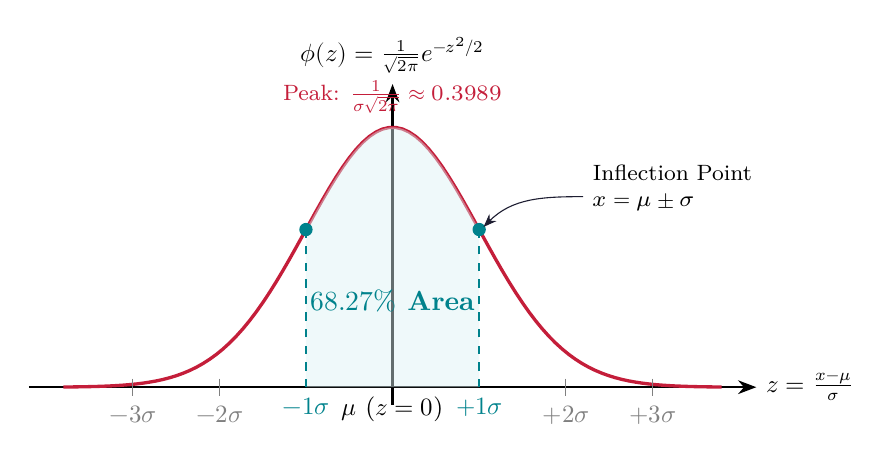
\begin{tikzpicture}[scale=1.1, every node/.style={font=\small}]
  % Axes
  \draw[-Stealth, thick] (-4.2, 0) -- (4.2, 0) node[right] {$z = \frac{x-\mu}{\sigma}$};
  \draw[-Stealth, thick] (0, -0.2) -- (0, 3.5) node[above] {$\phi(z) = \frac{1}{\sqrt{2\pi}} e^{-z^2/2}$};

  % Bell curve formula plot
  % Peak at z=0 is 1/sqrt(2pi) = 0.3989 -> scaled by 7.5 gives y = 3.0
  \draw[very thick, color=myred, domain=-3.8:3.8, samples=100]
    plot (\x, {3.0*exp(-(\x)^2/2)});

  % Shading 1-sigma central zone
  \fill[fill=hdrteal, fill opacity=0.45, domain=-1:1, samples=60]
    (-1,0) -- plot (\x, {3.0*exp(-(\x)^2/2)}) -- (1,0) -- cycle;

  % Inflection point markers at z = -1 and z = +1
  % Height at z=1 is 3.0*exp(-0.5) = 1.82
  \draw[thick, dashed, color=myteal] (-1, 0) node[below] {$-1\sigma$} -- (-1, 1.82);
  \filldraw[color=myteal] (-1, 1.82) circle (2pt);

  \draw[thick, dashed, color=myteal] (1, 0) node[below] {$+1\sigma$} -- (1, 1.82);
  \filldraw[color=myteal] (1, 1.82) circle (2pt);

  % 2-sigma and 3-sigma tick markers
  \draw[thin, color=gray] (-2, 0.1) -- (-2, -0.1) node[below] {$-2\sigma$};
  \draw[thin, color=gray] (2, 0.1) -- (2, -0.1) node[below] {$+2\sigma$};
  \draw[thin, color=gray] (-3, 0.1) -- (-3, -0.1) node[below] {$-3\sigma$};
  \draw[thin, color=gray] (3, 0.1) -- (3, -0.1) node[below] {$+3\sigma$};
  \node[below] at (0, 0) {$\mu$ ($z=0$)};

  % Annotations
  \node[color=myteal, font=\bfseries] at (0, 1.0) {$68.27\%$ Area};
  \node[above, color=myred, font=\footnotesize] at (0, 3.05) {Peak: $\frac{1}{\sigma\sqrt{2\pi}} \approx 0.3989$};

  \draw[-Stealth, thin, color=mydark] (2.2, 2.2) to[out=180, in=45] (1.05, 1.85);
  \node[right, font=\footnotesize, align=left] at (2.2, 2.3) {Inflection Point\\$x = \mu \pm \sigma$};
\end{tikzpicture}
\end{center}
\end{tcolorbox}

\subsection{Standard Normal Distribution and \texorpdfstring{$\Phi(z)$}{Phi(z)} Function}
When $\mu = 0$ and $\sigma = 1$, the variable is denoted $Z \sim \mathcal{N}(0, 1)$ with standard normal PDF $\phi(z) = \frac{1}{\sqrt{2\pi}} e^{-z^2/2}$ and CDF:
\begin{equation}
  \Phi(z) = P(Z \le z) = \frac{1}{\sqrt{2\pi}} \int_{-\infty}^z e^{-u^2/2} \, du
\end{equation}
By symmetry:
\begin{equation}
  \Phi(-z) = 1 - \Phi(z) \qquad \text{and} \qquad P(a \le X \le b) = \Phi\left(\frac{b - \mu}{\sigma}\right) - \Phi\left(\frac{a - \mu}{\sigma}\right)
\end{equation}

% ───────────────────────────────────────────────────────────────────────────────
\section{The Exponential Distribution}
% ───────────────────────────────────────────────────────────────────────────────

The \textbf{Exponential distribution} models the continuous time elapsed between independent random events occurring at a constant average rate $\lambda > 0$ (such as service times, component lifetimes, and inter-arrival times in queueing systems).

\begin{tcolorbox}[defbox, title={\textbf{Definition: Exponential Distribution $\mathbf{Exp(\lambda)}$}}]
A continuous random variable $X$ has an \textbf{Exponential distribution} with rate parameter $\lambda > 0$ ($X \sim \text{Exp}(\lambda)$) if its PDF is:
\begin{equation}
  f_X(x) =
  \begin{cases}
    \lambda e^{-\lambda x}, & x \ge 0 \\[3pt]
    0, & x < 0
  \end{cases}
\end{equation}
\end{tcolorbox}

\subsection{Derivation of CDF, Mean, Variance and MGF}
\begin{enumerate}[leftmargin=*, itemsep=3pt]
  \item \textbf{Cumulative Distribution Function (CDF):} For $x \ge 0$:
  \begin{equation}
    F_X(x) = \int_0^x \lambda e^{-\lambda t} \, dt = \left[-e^{-\lambda t}\right]_0^x = 1 - e^{-\lambda x}
  \end{equation}
  The survival (tail) probability is:
  \begin{equation}
    P(X > x) = 1 - F_X(x) = e^{-\lambda x}
  \end{equation}
  \item \textbf{Moment Generating Function (MGF):} For $t < \lambda$:
  \begin{equation}
    M_X(t) = \int_0^\infty e^{tx} \lambda e^{-\lambda x} \, dx = \lambda \int_0^\infty e^{-(\lambda - t)x} \, dx = \frac{\lambda}{\lambda - t} = \left(1 - \frac{t}{\lambda}\right)^{-1}
  \end{equation}
  Expanding in powers of $t/\lambda$:
  \begin{equation}
    M_X(t) = 1 + \frac{t}{\lambda} + \frac{t^2}{\lambda^2} + \frac{t^3}{\lambda^3} + \cdots = 1 + \left(\frac{1}{\lambda}\right) t + \left(\frac{2}{\lambda^2}\right) \frac{t^2}{2!} + \cdots
  \end{equation}
  \item \textbf{Mean and Variance:}
  \begin{equation}
    \mu = E[X] = \frac{1}{\lambda}, \qquad E[X^2] = \frac{2}{\lambda^2} \implies \operatorname{Var}(X) = E[X^2] - (E[X])^2 = \frac{2}{\lambda^2} - \frac{1}{\lambda^2} = \frac{1}{\lambda^2}
  \end{equation}
  Standard deviation is $\sigma = \frac{1}{\lambda}$. Notice that for the Exponential distribution: $\sigma = \mu$.
\end{enumerate}

\subsection{The Memoryless Property (Markov Property)}
\begin{tcolorbox}[examplebox, title={\textbf{Theorem: Memoryless Property of the Exponential Distribution}}]
Let $X \sim \text{Exp}(\lambda)$. For any non-negative time increments $s, t \ge 0$:
\begin{equation}
  P(X > s + t \mid X > s) = P(X > t)
\end{equation}
\textbf{Proof:} Using the conditional probability definition and $P(X > x) = e^{-\lambda x}$:
\begin{align}
  P(X > s + t \mid X > s) &= \frac{P(\{X > s + t\} \cap \{X > s\})}{P(X > s)} \nonumber \\[4pt]
                          &= \frac{P(X > s + t)}{P(X > s)} = \frac{e^{-\lambda(s+t)}}{e^{-\lambda s}} = \frac{e^{-\lambda s} e^{-\lambda t}}{e^{-\lambda s}} = e^{-\lambda t} = P(X > t)
\end{align}
\textit{Physical Interpretation:} If a semiconductor component has survived $s$ hours without failing, the probability that it survives an additional $t$ hours is identical to the probability that a brand-new component survives $t$ hours. The component suffers no wear-out aging over time!
\end{tcolorbox}

\begin{tcolorbox}[tikzbox, title={\textbf{TikZ Plot: Exponential Probability Density Functions for Different Rates $\lambda$}}]
\begin{center}
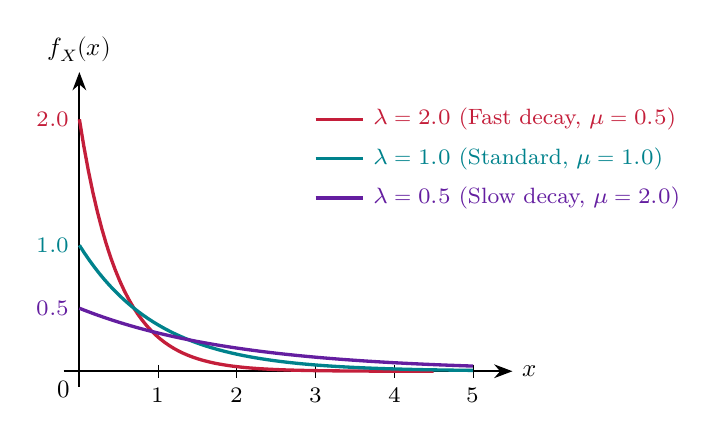
\begin{tikzpicture}[scale=1.0, every node/.style={font=\small}]
  % Axes
  \draw[-Stealth, thick] (-0.2, 0) -- (5.5, 0) node[right] {$x$};
  \draw[-Stealth, thick] (0, -0.2) -- (0, 3.8) node[above] {$f_X(x)$};

  % Ticks
  \foreach \x in {1,2,3,4,5} {
    \draw (\x, 0.08) -- (\x, -0.08) node[below] {\footnotesize $\x$};
  }
  \node[below left] at (0,0) {$0$};

  % Curves:
  % lambda = 2.0: peak at (0, 3.2), scale: 2.0 -> y=3.2
  \draw[very thick, color=myred, domain=0:4.5, samples=80]
    plot (\x, {3.2*exp(-2.0*\x)});
  \node[left, color=myred] at (0, 3.2) {\footnotesize $2.0$};

  % lambda = 1.0: peak at (0, 1.6)
  \draw[very thick, color=myteal, domain=0:5.0, samples=80]
    plot (\x, {1.6*exp(-1.0*\x)});
  \node[left, color=myteal] at (0, 1.6) {\footnotesize $1.0$};

  % lambda = 0.5: peak at (0, 0.8)
  \draw[very thick, color=mypurple, domain=0:5.0, samples=80]
    plot (\x, {0.8*exp(-0.5*\x)});
  \node[left, color=mypurple] at (0, 0.8) {\footnotesize $0.5$};

  % Legend
  \draw[very thick, color=myred] (3.0, 3.2) -- (3.6, 3.2) node[right, font=\footnotesize] {$\lambda = 2.0$ (Fast decay, $\mu=0.5$)};
  \draw[very thick, color=myteal] (3.0, 2.7) -- (3.6, 2.7) node[right, font=\footnotesize] {$\lambda = 1.0$ (Standard, $\mu=1.0$)};
  \draw[very thick, color=mypurple] (3.0, 2.2) -- (3.6, 2.2) node[right, font=\footnotesize] {$\lambda = 0.5$ (Slow decay, $\mu=2.0$)};
\end{tikzpicture}
\end{center}
\end{tcolorbox}

% ───────────────────────────────────────────────────────────────────────────────
\section{The Gamma Distribution and Its Properties}
% ───────────────────────────────────────────────────────────────────────────────

The \textbf{Gamma distribution} is a versatile two-parameter continuous distribution that extends the exponential distribution to model the waiting time until the occurrence of $\alpha$ successive Poisson events, as well as lifetime data exhibiting wear-out characteristics.

\begin{tcolorbox}[defbox, title={\textbf{Definition: The Gamma Function $\Gamma(\alpha)$}}]
The complete \textbf{Eulerian Gamma Function} is defined for all $\alpha > 0$ by the improper definite integral:
\begin{equation}
  \Gamma(\alpha) = \int_0^\infty u^{\alpha - 1} e^{-u} \, du
\end{equation}
\textbf{Fundamental Properties of $\Gamma(\alpha)$:}
\begin{enumerate}[leftmargin=*, itemsep=2pt]
  \item \textbf{Recurrence Relation:} $\Gamma(\alpha + 1) = \alpha \Gamma(\alpha)$ (integrating by parts).
  \item \textbf{Integer Factorial:} For any positive integer $n \in \mathbb{N}$: $\Gamma(n) = (n - 1)!$ with $\Gamma(1) = 0! = 1$.
  \item \textbf{Half-Integer Values:} $\Gamma\left(\frac{1}{2}\right) = \sqrt{\pi}$, from which $\Gamma\left(\frac{3}{2}\right) = \frac{1}{2}\sqrt{\pi}, \; \Gamma\left(\frac{5}{2}\right) = \frac{3}{4}\sqrt{\pi}$.
\end{enumerate}
\end{tcolorbox}

\begin{tcolorbox}[formulabox, title={\textbf{Two-Parameter Gamma Density $\mathbf{Gamma(\alpha, \beta)}$}}]
A random variable $X$ follows a \textbf{Gamma distribution} with shape parameter $\alpha > 0$ and rate parameter $\beta > 0$ (scale parameter $\theta = 1/\beta$) if its PDF is:
\begin{equation}
  f_X(x) =
  \begin{cases}
    \dfrac{\beta^\alpha}{\Gamma(\alpha)} x^{\alpha - 1} e^{-\beta x}, & x > 0 \\[8pt]
    0, & x \le 0
  \end{cases}
\end{equation}
\end{tcolorbox}

\subsection{Derivation of Mean, Variance and MGF of Gamma Distribution}
\begin{tcolorbox}[examplebox, title={\textbf{Rigorous Derivation: Moments of Gamma Distribution}}]
Using the MGF definition for $t < \beta$:
\begin{align}
  M_X(t) = \int_0^\infty e^{tx} \cdot \frac{\beta^\alpha}{\Gamma(\alpha)} x^{\alpha-1} e^{-\beta x} \, dx = \frac{\beta^\alpha}{\Gamma(\alpha)} \int_0^\infty x^{\alpha-1} e^{-(\beta - t)x} \, dx
\end{align}
Substitute $u = (\beta - t)x \implies x = \frac{u}{\beta - t}$ and $dx = \frac{du}{\beta - t}$:
\begin{equation}
  M_X(t) = \frac{\beta^\alpha}{\Gamma(\alpha)} \int_0^\infty \left(\frac{u}{\beta - t}\right)^{\alpha-1} e^{-u} \frac{du}{\beta - t} = \frac{\beta^\alpha}{(\beta - t)^\alpha} \cdot \underbrace{\frac{1}{\Gamma(\alpha)} \int_0^\infty u^{\alpha-1} e^{-u} du}_{= 1} = \left(1 - \frac{t}{\beta}\right)^{-\alpha}
\end{equation}
Expanding $(1 - t/\beta)^{-\alpha}$ using the generalized binomial theorem:
\begin{align}
  M_X(t) &= 1 + (-\alpha)\left(-\frac{t}{\beta}\right) + \frac{(-\alpha)(-\alpha-1)}{2!} \left(-\frac{t}{\beta}\right)^2 + \cdots \nonumber \\[3pt]
         &= 1 + \left(\frac{\alpha}{\beta}\right) t + \frac{\alpha(\alpha+1)}{\beta^2} \frac{t^2}{2!} + \cdots
\end{align}
Equating coefficients of $t$ and $t^2/2!$:
\begin{align}
  E[X] &= \mu = \frac{\alpha}{\beta} \\[3pt]
  E[X^2] &= \frac{\alpha(\alpha+1)}{\beta^2} \implies \operatorname{Var}(X) = E[X^2] - (E[X])^2 = \frac{\alpha^2 + \alpha}{\beta^2} - \frac{\alpha^2}{\beta^2} = \frac{\alpha}{\beta^2}
\end{align}
\end{tcolorbox}

\subsection{Special Cases and Reproductive Properties of Gamma Distribution}
\begin{enumerate}[leftmargin=*, itemsep=3pt]
  \item \textbf{Exponential Distribution Special Case:} When shape parameter $\alpha = 1$:
  \begin{equation}
    f_X(x) = \frac{\beta^1}{\Gamma(1)} x^{1-1} e^{-\beta x} = \beta e^{-\beta x} \equiv \text{Exp}(\beta)
  \end{equation}
  \item \textbf{Erlang Distribution:} When shape parameter $\alpha = k$ is a positive integer ($k \in \mathbb{N}$), the distribution represents the sum of $k$ independent and identically distributed $\text{Exp}(\beta)$ variables.
  \item \textbf{Chi-Square ($\chi^2$) Distribution Connection:} Substituting $\alpha = \frac{n}{2}$ and $\beta = \frac{1}{2}$ into the Gamma PDF yields:
  \begin{equation}
    f_X(x) = \frac{(1/2)^{n/2}}{\Gamma(n/2)} x^{n/2 - 1} e^{-x/2} \equiv \chi^2(n) \quad (\text{Chi-square with } n \text{ degrees of freedom})
  \end{equation}
  \item \textbf{Reproductive (Additive) Property:} If $X_1 \sim \text{Gamma}(\alpha_1, \beta)$ and $X_2 \sim \text{Gamma}(\alpha_2, \beta)$ are independent random variables sharing the \textit{same} rate parameter $\beta$, then:
  \begin{equation}
    M_{X_1+X_2}(t) = M_{X_1}(t) \cdot M_{X_2}(t) = \left(1 - \frac{t}{\beta}\right)^{-\alpha_1} \cdot \left(1 - \frac{t}{\beta}\right)^{-\alpha_2} = \left(1 - \frac{t}{\beta}\right)^{-(\alpha_1+\alpha_2)}
  \end{equation}
  By the uniqueness theorem of MGFs:
  \begin{equation}
    X_1 + X_2 \sim \text{Gamma}(\alpha_1 + \alpha_2, \beta)
  \end{equation}
\end{enumerate}

\begin{tcolorbox}[tikzbox, title={\textbf{TikZ Plot: Gamma Family PDFs for $\beta = 1.0$ and Varying Shape Parameter $\alpha$}}]
\begin{center}
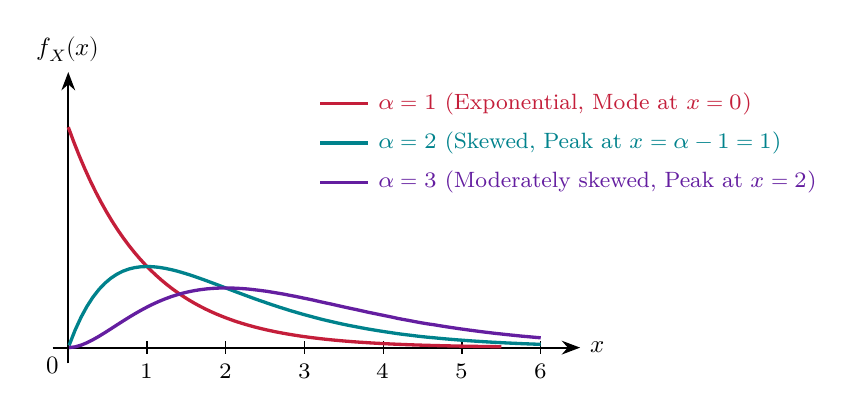
\begin{tikzpicture}[scale=1.0, every node/.style={font=\small}]
  % Axes
  \draw[-Stealth, thick] (-0.2, 0) -- (6.5, 0) node[right] {$x$};
  \draw[-Stealth, thick] (0, -0.2) -- (0, 3.5) node[above] {$f_X(x)$};

  % Ticks
  \foreach \x in {1,2,3,4,5,6} {
    \draw (\x, 0.08) -- (\x, -0.08) node[below] {\footnotesize $\x$};
  }
  \node[below left] at (0,0) {$0$};

  % alpha = 1: f(x) = e^(-x) (Exponential, monotonic decreasing)
  \draw[very thick, color=myred, domain=0:5.5, samples=80]
    plot (\x, {2.8*exp(-\x)});

  % alpha = 2: f(x) = x * e^(-x), peak at x=1 with value 1/e = 0.368 -> scaled: 2.8*0.368 = 1.03
  \draw[very thick, color=myteal, domain=0.01:6.0, samples=80]
    plot (\x, {2.8*\x*exp(-\x)});

  % alpha = 3: f(x) = (x^2 / 2) * e^(-x), peak at x=2 with value 4/(2*e^2) = 0.271 -> scaled: 2.8*0.271 = 0.76
  \draw[very thick, color=mypurple, domain=0.01:6.0, samples=80]
    plot (\x, {1.4*(\x)^2*exp(-\x)});

  % Legend
  \draw[very thick, color=myred] (3.2, 3.1) -- (3.8, 3.1) node[right, font=\footnotesize] {$\alpha = 1$ (Exponential, Mode at $x=0$)};
  \draw[very thick, color=myteal] (3.2, 2.6) -- (3.8, 2.6) node[right, font=\footnotesize] {$\alpha = 2$ (Skewed, Peak at $x = \alpha-1 = 1$)};
  \draw[very thick, color=mypurple] (3.2, 2.1) -- (3.8, 2.1) node[right, font=\footnotesize] {$\alpha = 3$ (Moderately skewed, Peak at $x = 2$)};
\end{tikzpicture}
\end{center}
\end{tcolorbox}

\newpage
% ===============================================================================
% MANDATORY QUICK REVISION PAGE
% ===============================================================================
\begin{center}
  {\large\bfseries\color{myred} Quick Revision --- Module 2}\\[1pt]
  {\small\color{mydark} Continuous Probability Distributions $|$ BS-M301}
\end{center}
\noindent{\color{myred}\rule{\linewidth}{1.0pt}}
\vspace{1pt}

\begin{tcolorbox}[formulabox, top=2pt, bottom=2pt, title={\textbf{Key Formulas and Continuous Distribution Densities at a Glance}}]
\renewcommand{\arraystretch}{0.96}
\setlength{\tabcolsep}{3.5pt}
\begin{tabularx}{\linewidth}{B{3.8cm} X}
Continuous PDF Conditions & $f_X(x) \ge 0, \quad \int_{-\infty}^\infty f_X(x) dx = 1, \quad P(a \le X \le b) = \int_a^b f_X(x) dx$ \\[0.2pt]
CDF to PDF Relationship & $F_X(x) = \int_{-\infty}^x f_X(t) dt, \quad f_X(x) = \frac{d}{dx}F_X(x), \quad P(X = c) = 0$ \\[0.2pt]
Continuous Expectation & $E[X] = \mu = \int_{-\infty}^\infty x f_X(x) dx, \quad \operatorname{Var}(X) = E[X^2] - \mu^2$ \\[0.2pt]
MGF Formula & $M_X(t) = E[e^{tX}] = \int_{-\infty}^\infty e^{tx} f_X(x) dx, \quad \mu_r' = \left.\frac{d^r M_X(t)}{dt^r}\right|_{t=0}$ \\[0.2pt]
Normal PDF $\mathcal{N}(\mu, \sigma^2)$ & $f(x) = \frac{1}{\sigma\sqrt{2\pi}} \exp\left(-\frac{(x-\mu)^2}{2\sigma^2}\right), \quad M_X(t) = \exp\left(\mu t + \frac{1}{2}\sigma^2 t^2\right)$ \\[0.2pt]
Standard Normal $Z$ & $Z = \frac{X-\mu}{\sigma} \sim \mathcal{N}(0, 1), \quad \phi(z) = \frac{1}{\sqrt{2\pi}} e^{-z^2/2}, \quad \Phi(-z) = 1-\Phi(z)$ \\[0.2pt]
Normal Moments & All odd $\mu_{2k+1} = 0, \quad \mu_2 = \sigma^2, \quad \mu_4 = 3\sigma^4, \quad \beta_1 = 0, \; \beta_2 = 3$ \\[0.2pt]
Exponential PDF $\text{Exp}(\lambda)$ & $f(x) = \lambda e^{-\lambda x} \; (x \ge 0), \quad F(x) = 1 - e^{-\lambda x}, \quad \mu = \frac{1}{\lambda}, \; \sigma^2 = \frac{1}{\lambda^2}$ \\[0.2pt]
Memoryless Property & $P(X > s+t \mid X > s) = P(X > t) \quad \text{(Unique to Exponential)}$ \\[0.2pt]
Gamma Function & $\Gamma(\alpha) = \int_0^\infty u^{\alpha-1} e^{-u} du, \quad \Gamma(\alpha+1) = \alpha \Gamma(\alpha), \quad \Gamma(1/2) = \sqrt{\pi}$ \\[0.2pt]
Gamma PDF $\text{Gamma}(\alpha, \beta)$ & $f(x) = \frac{\beta^\alpha}{\Gamma(\alpha)} x^{\alpha-1} e^{-\beta x}, \quad \mu = \frac{\alpha}{\beta}, \quad \sigma^2 = \frac{\alpha}{\beta^2}, \quad M_X(t) = \left(1-\frac{t}{\beta}\right)^{-\alpha}$ \\
\end{tabularx}
\end{tcolorbox}

\vspace{1pt}

\begin{tcolorbox}[defbox, top=2pt, bottom=2pt, title={\textbf{One-Line Definitions}}]
\begin{itemize}[leftmargin=*, itemsep=-0.5pt, topsep=0pt, parsep=0pt]
  \item \textbf{Continuous Random Variable:} Variable taking any real value in an interval, with single-point probability $P(X=c)=0$.
  \item \textbf{Probability Density Function (PDF):} Non-negative derivative of the CDF whose integral over an interval gives probability.
  \item \textbf{Normal Distribution:} Symmetrical mesokurtic bell curve fully governed by location $\mu$ and scale $\sigma$.
  \item \textbf{Inflection Points:} Points where curvature flips concavity, situated at precisely $x = \mu \pm \sigma$ for a normal curve.
  \item \textbf{Standard Score ($Z$):} Dimensionless measure $Z = (X-\mu)/\sigma$ expressing deviation from mean in units of $\sigma$.
  \item \textbf{Exponential Distribution:} Only continuous distribution possessing memorylessness, modelling Poisson inter-arrival times.
  \item \textbf{Memoryless Property:} Independence of future remaining lifetime from past survival duration: $P(X>s+t \mid X>s) = P(X>t)$.
  \item \textbf{Gamma Function ($\Gamma(\alpha)$):} Generalized factorial integral extending $n!$ to all real positive numbers ($\Gamma(n) = (n-1)!$).
  \item \textbf{Erlang Distribution:} Gamma distribution with integer shape parameter $\alpha = k$, representing sum of $k$ independent exponentials.
  \item \textbf{Reproductive Property:} Closure under convolution: sum of independent Gammas with same $\beta$ yields another Gamma.
\end{itemize}
\end{tcolorbox}

\newpage

\begin{tcolorbox}[exambox, title={\textbf{Frequently Asked / Viva Questions (Part 1)}}]
\begin{enumerate}[topsep=0pt, label=\textbf{Q\arabic*.}, itemsep=3.2pt]
  \item \Q{Why is the probability of a continuous random variable taking an exact value zero ($P(X = c) = 0$)?}
  By definition, $P(X = c) = \int_c^c f_X(x) \, dx = 0$. Since an interval contains uncountably infinitely many points, the probability mass allocated to any isolated geometric point vanishes, even though the event is not impossible in reality.

  \item \Q{Can a probability density function exceed unity ($f_X(x) > 1$)? Explain with an example.}
  Yes! Unlike discrete PMFs where $p(x) \le 1$, a continuous PDF represents probability \textit{density} per unit width, not probability. For example, for $X \sim U[0, 0.2]$, $f_X(x) = 1/(0.2 - 0) = 5.0 > 1$, while the total integral $\int_0^{0.2} 5.0 \, dx = 1.0$ is fully preserved.

  \item \Q{Derive the Moment Generating Function of the standard normal distribution $Z \sim \mathcal{N}(0, 1)$.}
  $M_Z(t) = \frac{1}{\sqrt{2\pi}} \int_{-\infty}^\infty e^{tz} e^{-z^2/2} dz = \frac{1}{\sqrt{2\pi}} \int_{-\infty}^\infty e^{-(z^2 - 2tz)/2} dz$. Completing the square: $z^2 - 2tz = (z-t)^2 - t^2$. Factoring out $e^{t^2/2}$: $M_Z(t) = e^{t^2/2} \frac{1}{\sqrt{2\pi}} \int_{-\infty}^\infty e^{-(z-t)^2/2} dz = e^{t^2/2} \cdot 1 = e^{t^2/2}$.

  \item \Q{Prove that all odd central moments of a Normal distribution are identically zero.}
  $\mu_{2k+1} = \frac{1}{\sigma\sqrt{2\pi}} \int_{-\infty}^\infty (x-\mu)^{2k+1} e^{-(x-\mu)^2/(2\sigma^2)} dx$. Substituting $u = x - \mu$: the integrand $u^{2k+1} e^{-u^2/(2\sigma^2)}$ is an odd function of $u$ ($g(-u) = -g(u)$) integrated over symmetric limits $(-\infty, \infty)$, which integrates to zero.

  \item \Q{Where do the inflection points of a normal probability curve occur?}
  Equating the second derivative to zero: $f''(x) = \left[\frac{(x-\mu)^2}{\sigma^4} - \frac{1}{\sigma^2}\right] f(x) = 0 \implies (x-\mu)^2 = \sigma^2 \implies x = \mu \pm \sigma$. The curve transitions from concave downwards to concave upwards at exactly one standard deviation on either side of the mean.

  \item \Q{State and prove the memoryless property of the Exponential distribution.}
  $P(X > s + t \mid X > s) = \frac{P(X > s + t)}{P(X > s)} = \frac{e^{-\lambda(s+t)}}{e^{-\lambda s}} = e^{-\lambda t} = P(X > t)$. The conditional probability that a component lasts $t$ more units given it has lasted $s$ units is independent of $s$.

  \item \Q{What is the physical connection between the Poisson process and the Exponential distribution?}
  In a Poisson process with rate $\lambda$, the number of event arrivals in interval $t$ follows $\text{Poisson}(\lambda t)$. The waiting time $T$ until the first arrival exceeds $t$ if and only if zero arrivals occur in $[0, t]$: $P(T > t) = P(N(t) = 0) = \frac{(\lambda t)^0 e^{-\lambda t}}{0!} = e^{-\lambda t}$. Thus, the inter-arrival time $T$ is exponentially distributed with parameter $\lambda$.
\end{enumerate}
\end{tcolorbox}

\newpage

\begin{tcolorbox}[exambox, top=3pt, bottom=3pt, title={\textbf{Frequently Asked / Viva Questions (Part 2)}}]
\begin{enumerate}[topsep=0pt, label=\textbf{Q\arabic*.}, itemsep=1.8pt, start=8]
  \item \Q{Prove that $\Gamma(1/2) = \sqrt{\pi}$.}
  $\Gamma(1/2) = \int_0^\infty u^{-1/2} e^{-u} du$. Substituting $u = z^2/2 \implies du = z dz$: $\Gamma(1/2) = \int_0^\infty \frac{\sqrt{2}}{z} e^{-z^2/2} z dz = \sqrt{2} \int_0^\infty e^{-z^2/2} dz$. By symmetry: $\int_0^\infty e^{-z^2/2} dz = \frac{1}{2} \int_{-\infty}^\infty e^{-z^2/2} dz = \frac{\sqrt{2\pi}}{2} = \sqrt{\frac{\pi}{2}}$. Multiplying by $\sqrt{2}$ yields $\Gamma(1/2) = \sqrt{\pi}$.

  \item \Q{How is the Chi-Square ($\chi^2$) distribution obtained as a special case of the Gamma distribution?}
  Setting shape parameter $\alpha = n/2$ and rate parameter $\beta = 1/2$ in the Gamma PDF yields $f(x) = \frac{(1/2)^{n/2}}{\Gamma(n/2)} x^{n/2 - 1} e^{-x/2}$, which is the standard definition of the Chi-Square distribution with $n$ degrees of freedom.

  \item \Q{State the reproductive property of independent Normal random variables.}
  If $X_1 \sim \mathcal{N}(\mu_1, \sigma_1^2)$ and $X_2 \sim \mathcal{N}(\mu_2, \sigma_2^2)$ are independent, any linear combination $Y = aX_1 + bX_2$ is also normally distributed: $Y \sim \mathcal{N}(a\mu_1 + b\mu_2, a^2\sigma_1^2 + b^2\sigma_2^2)$. This follows directly from multiplying their MGFs.
\end{enumerate}
\end{tcolorbox}

\vspace{2pt}

\begin{tcolorbox}[tikzbox, top=3pt, bottom=3pt, title={\textbf{Summary Matrix: Comprehensive Comparison of Continuous Distributions}}]
\par\vspace{1pt}\noindent
\begingroup
\setlength{\tabcolsep}{3.5pt}
\setlength{\extrarowheight}{1.0pt}
\renewcommand{\arraystretch}{1.12}
\begin{tabularx}{\linewidth}{|B{2.5cm}|B{3.8cm}|B{2.2cm}|B{2.2cm}|Y|}
\hline
\textbf{Distribution} & \textbf{Probability Density Function (PDF)} & \textbf{Mean ($E[X]$)} & \textbf{Variance ($\sigma^2$)} & \textbf{Key Engineering Application} \\
\hline
Uniform $U[a, b]$ & $f(x) = \frac{1}{b-a}, \quad x \in [a, b]$ & $\frac{a+b}{2}$ & $\frac{(b-a)^2}{12}$ & Quantization noise in ADC systems. \\
\hline
Normal $\mathcal{N}(\mu, \sigma^2)$ & $f(x) = \frac{1}{\sigma\sqrt{2\pi}} e^{-(x-\mu)^2/(2\sigma^2)}$ & $\mu$ & $\sigma^2$ & Thermal Gaussian noise; Central Limit Theorem. \\
\hline
Exponential $\text{Exp}(\lambda)$ & $f(x) = \lambda e^{-\lambda x}, \quad x \ge 0$ & $\frac{1}{\lambda}$ & $\frac{1}{\lambda^2}$ & Lifetime of electronic parts; queueing theory. \\
\hline
Gamma $(\alpha, \beta)$ & $f(x) = \frac{\beta^\alpha}{\Gamma(\alpha)} x^{\alpha-1} e^{-\beta x}, \; x > 0$ & $\frac{\alpha}{\beta}$ & $\frac{\alpha}{\beta^2}$ & Waiting time for $\alpha$ events; reliability engineering. \\
\hline
Chi-Square $\chi^2(n)$ & $f(x) = \frac{(1/2)^{n/2}}{\Gamma(n/2)} x^{n/2-1} e^{-x/2}$ & $n$ & $2n$ & Goodness-of-fit testing; sample variance distribution. \\
\hline
\end{tabularx}
\endgroup
\end{tcolorbox}


% -- Module 3 -----------------------------------------------------------------
\modulestart{3}{Bivariate Distributions and Their Fundamental Properties}

\section{Bivariate Distributions and Their Fundamental Properties}
% ───────────────────────────────────────────────────────────────────────────────

In numerous engineering problems, physical phenomena involve the simultaneous observation of two interdependent random quantities, such as the in-phase and quadrature components of an RF communication signal $(I, Q)$, transmitter voltage and received current $(V, I)$, or temperature and humidity. These are modeled jointly as a \textbf{two-dimensional (bivariate) random variable} $(X, Y): \Omega \to \mathbb{R}^2$.

\begin{tcolorbox}[defbox, title={\textbf{Definition: Joint Probability Mass and Density Functions}}]
\textbf{Discrete Bivariate Case (Joint PMF):}
Let $(X, Y)$ take values in a countable set of pairs $(x_i, y_j)$. The \textbf{Joint PMF} is:
\begin{equation}
  p_{XY}(x_i, y_j) = P(X = x_i, Y = y_j)
\end{equation}
Axioms: (1) $p_{XY}(x_i, y_j) \ge 0, \quad \forall (i, j)$, \quad (2) $\displaystyle\sum_{i} \sum_{j} p_{XY}(x_i, y_j) = 1$.

\textbf{Continuous Bivariate Case (Joint PDF):}
$(X, Y)$ is jointly continuous if there exists an integrable surface $f_{XY}: \mathbb{R}^2 \to \mathbb{R}$ such that for any two-dimensional region $D \subseteq \mathbb{R}^2$:
\begin{equation}
  P((X, Y) \in D) = \iint_D f_{XY}(x, y) \, dx dy
\end{equation}
Axioms:
\begin{align}
  \textbf{Non-negativity:} \quad & f_{XY}(x, y) \ge 0, \quad \forall (x, y) \in \mathbb{R}^2 \\[4pt]
  \textbf{Unit Volume:} \quad & \int_{-\infty}^\infty \int_{-\infty}^\infty f_{XY}(x, y) \, dx dy = 1
\end{align}
\end{tcolorbox}

\subsection{Joint Cumulative Distribution Function (Joint CDF)}
The \textbf{Joint CDF} of $(X, Y)$ is defined as the probability of the infinite quadrant to the south-west of $(x, y)$:
\begin{equation}
  F_{XY}(x, y) = P(X \le x, Y \le y) =
  \begin{cases}
    \displaystyle\sum_{x_i \le x} \sum_{y_j \le y} p_{XY}(x_i, y_j), & \text{(Discrete)} \\[10pt]
    \displaystyle\int_{-\infty}^x \int_{-\infty}^y f_{XY}(u, v) \, dv du, & \text{(Continuous)}
  \end{cases}
\end{equation}

\begin{tcolorbox}[formulabox, title={\textbf{Properties of the Joint CDF and Recovery of Joint PDF}}]
\begin{enumerate}[leftmargin=*, itemsep=3pt]
  \item \textbf{Boundary Limits:}
  \begin{align}
    F_{XY}(-\infty, y) &= 0, \qquad F_{XY}(x, -\infty) = 0, \qquad F_{XY}(-\infty, -\infty) = 0 \\[2pt]
    F_{XY}(+\infty, +\infty) &= 1
  \end{align}
  \item \textbf{Marginal Recovery from Joint CDF:}
  \begin{equation}
    F_X(x) = \lim_{y \to +\infty} F_{XY}(x, y) = F_{XY}(x, \infty), \qquad F_Y(y) = \lim_{x \to +\infty} F_{XY}(x, y) = F_{XY}(\infty, y)
  \end{equation}
  \item \textbf{Recovery of Continuous Joint PDF by Partial Differentiation:}
  At every continuity point of $f_{XY}(x, y)$:
  \begin{equation}
    f_{XY}(x, y) = \frac{\partial^2}{\partial x \partial y} F_{XY}(x, y) = \frac{\partial^2}{\partial y \partial x} F_{XY}(x, y)
  \end{equation}
  \item \textbf{Rectangle Probability Rule:} For any rectangular region $[x_1, x_2] \times [y_1, y_2]$:
  \begin{align}
    P(x_1 < X \le x_2, \; y_1 < Y \le y_2) = \; & F_{XY}(x_2, y_2) - F_{XY}(x_1, y_2) \nonumber \\[2pt]
                                                & - F_{XY}(x_2, y_1) + F_{XY}(x_1, y_1) \ge 0
  \end{align}
\end{enumerate}
\end{tcolorbox}

\subsection{Marginal Distributions}
The individual distribution of one variable obtained by integrating or summing out the other variable over its entire support is termed the \textbf{marginal distribution}.
\begin{align}
  \textbf{Marginal PMFs:} \quad & p_X(x_i) = \sum_{j} p_{XY}(x_i, y_j), \qquad p_Y(y_j) = \sum_{i} p_{XY}(x_i, y_j) \\[4pt]
  \textbf{Marginal PDFs:} \quad & f_X(x) = \int_{-\infty}^\infty f_{XY}(x, y) \, dy, \qquad f_Y(y) = \int_{-\infty}^\infty f_{XY}(x, y) \, dx
\end{align}

\begin{tcolorbox}[tikzbox, title={\textbf{TikZ Schematic: Geometric Interpretation of Marginal Integration across Joint Support}}]
\begin{center}
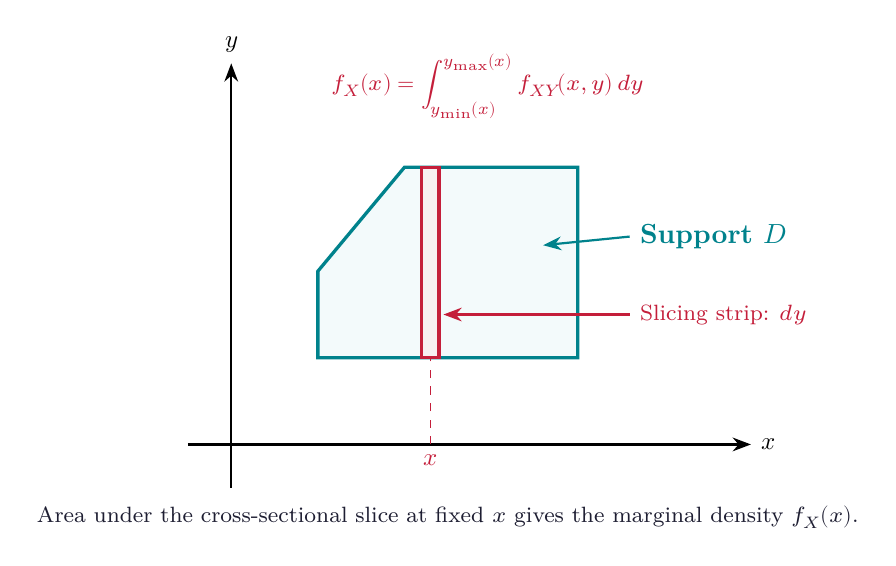
\begin{tikzpicture}[scale=1.1, every node/.style={font=\small}]
  % Axes
  \draw[-Stealth, thick] (-0.5, 0) -- (6.0, 0) node[right] {$x$};
  \draw[-Stealth, thick] (0, -0.5) -- (0, 4.4) node[above] {$y$};

  % Support region D
  \draw[very thick, color=myteal, fill=hdrteal, fill opacity=0.35]
    (1, 1) -- (4, 1) -- (4, 3.2) -- (2, 3.2) -- (1, 2) -- cycle;

  % Fixed x vertical strip
  \draw[very thick, color=myred, fill=hdrred, fill opacity=0.6] (2.2, 1) rectangle (2.4, 3.2);
  \draw[dashed, thin, color=myred] (2.3, 0) node[below] {$x$} -- (2.3, 1);

  % External Callouts on the right
  \draw[-Stealth, thick, color=myteal] (4.6, 2.4) node[right, font=\bfseries, color=myteal] {Support $D$} -- (3.6, 2.3);
  \draw[-Stealth, thick, color=myred] (4.6, 1.5) node[right, font=\footnotesize, color=myred] {Slicing strip: $dy$} -- (2.45, 1.5);

  % Annotations at top
  \node[above, color=myred, font=\footnotesize, align=center] at (3.0, 3.65) {
    $f_X(x) = \displaystyle\int_{y_{\min}(x)}^{y_{\max}(x)} f_{XY}(x, y) \, dy$
  };
  \node[below, color=mydark, font=\footnotesize] at (2.5, -0.6) {
    Area under the cross-sectional slice at fixed $x$ gives the marginal density $f_X(x)$.
  };
\end{tikzpicture}
\end{center}
\end{tcolorbox}

% ───────────────────────────────────────────────────────────────────────────────
\section{Conditional Distributions, Densities and Bayes' Rule}
% ───────────────────────────────────────────────────────────────────────────────

\begin{tcolorbox}[defbox, title={\textbf{Definition: Conditional Probability Density Function}}]
Given that the random variable $Y$ has taken on a specific numerical value $Y = y$ (where marginal density $f_Y(y) > 0$), the \textbf{conditional PDF} of $X$ given $Y = y$ is defined as:
\begin{equation}
  f_{X \mid Y}(x \mid y) = \frac{f_{XY}(x, y)}{f_Y(y)} = \frac{f_{XY}(x, y)}{\displaystyle\int_{-\infty}^\infty f_{XY}(u, y) \, du}
\end{equation}
Symmetrically, the conditional PDF of $Y$ given $X = x$ (with $f_X(x) > 0$) is:
\begin{equation}
  f_{Y \mid X}(y \mid x) = \frac{f_{XY}(x, y)}{f_X(x)} = \frac{f_{XY}(x, y)}{\displaystyle\int_{-\infty}^\infty f_{XY}(x, v) \, dv}
\end{equation}
Every conditional density satisfies the standard PDF axioms: $f_{X|Y}(x \mid y) \ge 0$ and $\int_{-\infty}^\infty f_{X|Y}(x \mid y) dx = 1$.
\end{tcolorbox}

\subsection{Conditional Expectation and the Tower Property}
\begin{itemize}[leftmargin=*, itemsep=3pt]
  \item \textbf{Conditional Expectation:} The mean of $X$ given $Y = y$ is a function of $y$:
  \begin{equation}
    E[X \mid Y = y] = \int_{-\infty}^\infty x f_{X \mid Y}(x \mid y) \, dx
  \end{equation}
  \item \textbf{Law of Iterated Expectations (Tower Property):}
  \begin{equation}
    E\left[E[X \mid Y]\right] = E[X]
  \end{equation}
  \textbf{Proof:}
  \begin{align}
    E\left[E[X \mid Y]\right] &= \int_{-\infty}^\infty \left(\int_{-\infty}^\infty x \frac{f_{XY}(x, y)}{f_Y(y)} dx\right) f_Y(y) \, dy \nonumber \\
                              &= \int_{-\infty}^\infty \int_{-\infty}^\infty x f_{XY}(x, y) \, dx dy = \int_{-\infty}^\infty x \left(\int_{-\infty}^\infty f_{XY}(x, y) dy\right) dx \nonumber \\
                              &= \int_{-\infty}^\infty x f_X(x) \, dx = E[X]
  \end{align}
  \item \textbf{Law of Total Variance (Eve's Law):}
  \begin{equation}
    \operatorname{Var}(X) = E[\operatorname{Var}(X \mid Y)] + \operatorname{Var}(E[X \mid Y])
  \end{equation}
  Total uncertainty equals the average unexplained variance plus the variance explained by $Y$.
\end{itemize}

\subsection{Bayes' Rule for Continuous and Mixed Random Variables}
\begin{tcolorbox}[formulabox, title={\textbf{Continuous and Mixed Formulations of Bayes' Rule}}]
\textbf{Continuous Inversion (Posterior Density):}
Equating $f_{XY}(x, y) = f_X(x) f_{Y|X}(y \mid x) = f_Y(y) f_{X|Y}(x \mid y)$:
\begin{equation}
  f_{X \mid Y}(x \mid y) = \frac{f_X(x) \cdot f_{Y \mid X}(y \mid x)}{f_Y(y)} = \frac{f_X(x) \cdot f_{Y \mid X}(y \mid x)}{\displaystyle\int_{-\infty}^\infty f_X(u) \cdot f_{Y \mid X}(y \mid u) \, du}
\end{equation}
where $f_X(x)$ is the \textit{prior density}, $f_{Y|X}(y \mid x)$ is the \textit{likelihood function}, and $f_{X|Y}(x \mid y)$ is the \textit{posterior density}.

\textbf{Discrete Hypothesis with Continuous Measurement (Signal Detection):}
Let $\{H_1, H_2, \dots, H_n\}$ be discrete transmitted symbols (priors $P(H_i)$) observed through continuous additive noise $Y$:
\begin{equation}
  P(H_k \mid Y = y) = \frac{P(H_k) \cdot f_{Y \mid H_k}(y)}{\displaystyle\sum_{i=1}^n P(H_i) \cdot f_{Y \mid H_i}(y)}
\end{equation}
\end{tcolorbox}

% ───────────────────────────────────────────────────────────────────────────────
\section{Bivariate Transformations and the Jacobian Method}
% ───────────────────────────────────────────────────────────────────────────────

When analyzing signal processing systems, inputs $(X, Y)$ are mapped into new output variables $(U, V)$ via mathematical functions $U = g_1(X, Y)$ and $V = g_2(X, Y)$.

\begin{tcolorbox}[defbox, title={\textbf{Theorem: Bivariate Jacobian Transformation}}]
Let $(X, Y)$ have joint PDF $f_{XY}(x, y)$ supported on set $D$. Let the transformation:
\begin{equation}
  u = g_1(x, y), \qquad v = g_2(x, y)
\end{equation}
define a one-to-one and invertible mapping from $D$ onto range $S$, with unique inverse:
\begin{equation}
  x = h_1(u, v), \qquad y = h_2(u, v)
\end{equation}
If the partial derivatives are continuous, the \textbf{Jacobian determinant} $J$ of the inverse transformation is:
\begin{equation}
  J = \frac{\partial(x, y)}{\partial(u, v)} = \det \begin{pmatrix} \dfrac{\partial x}{\partial u} & \dfrac{\partial x}{\partial v} \\[6pt] \dfrac{\partial y}{\partial u} & \dfrac{\partial y}{\partial v} \end{pmatrix} = \frac{\partial x}{\partial u}\frac{\partial y}{\partial v} - \frac{\partial x}{\partial v}\frac{\partial y}{\partial u}
\end{equation}
Then the joint PDF of $(U, V)$ over $S$ is given by:
\begin{equation}
  f_{UV}(u, v) = f_{XY}\left(h_1(u, v), h_2(u, v)\right) \cdot |J|
\end{equation}
where $|J|$ is the absolute value of the Jacobian determinant (representing the local area scaling factor: $dx dy = |J| du dv$).
\end{tcolorbox}

\begin{tcolorbox}[tikzbox, title={\textbf{TikZ Schematic: Area Element Transformation under Jacobian Mapping}}]
\begin{center}
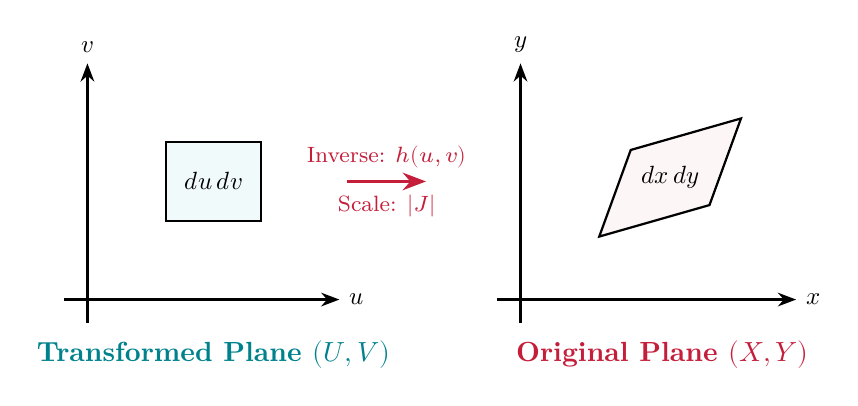
\begin{tikzpicture}[scale=1.0, every node/.style={font=\small}]
  % Left plane: (u, v)
  \begin{scope}[shift={(-3.5, 0)}]
    \draw[-Stealth, thick] (-0.3, 0) -- (3.2, 0) node[right] {$u$};
    \draw[-Stealth, thick] (0, -0.3) -- (0, 3.0) node[above] {$v$};

    \draw[thick, fill=hdrteal, fill opacity=0.4] (1, 1) rectangle (2.2, 2.0);
    \node at (1.6, 1.5) {$du \, dv$};
    \node[below, font=\bfseries, color=myteal] at (1.6, -0.4) {Transformed Plane $(U, V)$};
  \end{scope}

  % Mapping arrow
  \draw[-Stealth, very thick, color=myred] (-0.2, 1.5) -- (0.8, 1.5);
  \node[above, color=myred, font=\footnotesize] at (0.3, 1.55) {Inverse: $h(u,v)$};
  \node[below, color=myred, font=\footnotesize] at (0.3, 1.45) {Scale: $|J|$};

  % Right plane: (x, y)
  \begin{scope}[shift={(2.0, 0)}]
    \draw[-Stealth, thick] (-0.3, 0) -- (3.5, 0) node[right] {$x$};
    \draw[-Stealth, thick] (0, -0.3) -- (0, 3.0) node[above] {$y$};

    \draw[thick, fill=hdrred, fill opacity=0.4]
      (1, 0.8) -- (2.4, 1.2) -- (2.8, 2.3) -- (1.4, 1.9) -- cycle;
    \node at (1.9, 1.55) {$dx \, dy$};
    \node[below, font=\bfseries, color=myred] at (1.8, -0.4) {Original Plane $(X, Y)$};
  \end{scope}
\end{tikzpicture}
\end{center}
\end{tcolorbox}

% ───────────────────────────────────────────────────────────────────────────────
\section{Distributions of Sums and Quotients}
% ───────────────────────────────────────────────────────────────────────────────

\subsection{Distribution of the Sum $Z = X + Y$ (Convolution)}
\begin{tcolorbox}[examplebox, title={\textbf{Derivation: PDF of the Sum of Two Continuous Random Variables}}]
To find the PDF of $Z = X + Y$, introduce an auxiliary variable $W = X$.
The forward transformation is:
\begin{equation}
  z = x + y, \qquad w = x
\end{equation}
The unique inverse transformation is:
\begin{equation}
  x = w, \qquad y = z - w
\end{equation}
Computing the Jacobian determinant:
\begin{equation}
  J = \det \begin{pmatrix} \frac{\partial x}{\partial z} & \frac{\partial x}{\partial w} \\[4pt] \frac{\partial y}{\partial z} & \frac{\partial y}{\partial w} \end{pmatrix} = \det \begin{pmatrix} 0 & 1 \\ 1 & -1 \end{pmatrix} = (0)(-1) - (1)(1) = -1 \implies |J| = |-1| = 1
\end{equation}
The joint PDF of $(Z, W)$ is:
\begin{equation}
  f_{ZW}(z, w) = f_{XY}(w, z - w) \cdot |J| = f_{XY}(w, z - w)
\end{equation}
Integrating out the auxiliary variable $w$ yields the marginal PDF of the sum $Z$:
\begin{equation}
  f_Z(z) = \int_{-\infty}^\infty f_{ZW}(z, w) \, dw = \int_{-\infty}^\infty f_{XY}(w, z - w) \, dw
\end{equation}
If $X$ and $Y$ are \textbf{independent} ($f_{XY}(x, y) = f_X(x) f_Y(y)$), this becomes the fundamental \textbf{continuous convolution integral}:
\begin{equation}
  f_Z(z) = (f_X * f_Y)(z) = \int_{-\infty}^\infty f_X(w) f_Y(z - w) \, dw = \int_{-\infty}^\infty f_X(z - y) f_Y(y) \, dy
\end{equation}
\end{tcolorbox}

\subsection{Distribution of the Quotient $Z = X / Y$}
\begin{tcolorbox}[examplebox, title={\textbf{Derivation: PDF of the Quotient of Two Random Variables}}]
Let $Z = \frac{X}{Y}$. Introduce the auxiliary variable $W = Y$.
The forward transformation is:
\begin{equation}
  z = \frac{x}{y}, \qquad w = y \quad (w \ne 0)
\end{equation}
The inverse transformation is:
\begin{equation}
  x = z \cdot w, \qquad y = w
\end{equation}
The Jacobian determinant is:
\begin{equation}
  J = \det \begin{pmatrix} \frac{\partial x}{\partial z} & \frac{\partial x}{\partial w} \\[4pt] \frac{\partial y}{\partial z} & \frac{\partial y}{\partial w} \end{pmatrix} = \det \begin{pmatrix} w & z \\ 0 & 1 \end{pmatrix} = (w)(1) - (z)(0) = w \implies |J| = |w|
\end{equation}
The joint PDF of $(Z, W)$ is:
\begin{equation}
  f_{ZW}(z, w) = f_{XY}(z w, w) \cdot |w|
\end{equation}
Integrating out $w$ over $(-\infty, \infty)$ yields the general quotient density:
\begin{equation}
  f_Z(z) = \int_{-\infty}^\infty |w| f_{XY}(z w, w) \, dw
\end{equation}
If $X$ and $Y$ are independent:
\begin{equation}
  f_Z(z) = \int_{-\infty}^\infty |w| f_X(z w) f_Y(w) \, dw
\end{equation}
\end{tcolorbox}

\subsection{Quotient of Two Independent Standard Normals: The Cauchy Distribution}
\begin{tcolorbox}[examplebox, title={\textbf{Classic Result: Ratio of Independent Standard Normals follows Cauchy}}]
Let $X \sim \mathcal{N}(0, 1)$ and $Y \sim \mathcal{N}(0, 1)$ be independent. Their joint density is:
\begin{equation}
  f_{XY}(x, y) = \frac{1}{\sqrt{2\pi}} e^{-x^2/2} \cdot \frac{1}{\sqrt{2\pi}} e^{-y^2/2} = \frac{1}{2\pi} e^{-(x^2 + y^2)/2}
\end{equation}
Applying the quotient formula to $Z = X/Y$:
\begin{equation}
  f_Z(z) = \int_{-\infty}^\infty |w| \cdot \frac{1}{2\pi} e^{-(z^2 w^2 + w^2)/2} \, dw = \frac{1}{2\pi} \int_{-\infty}^\infty |w| e^{-\frac{w^2(1 + z^2)}{2}} \, dw
\end{equation}
Since the integrand is even with respect to $w$:
\begin{equation}
  f_Z(z) = \frac{2}{2\pi} \int_0^\infty w e^{-\frac{w^2(1 + z^2)}{2}} \, dw = \frac{1}{\pi} \int_0^\infty w e^{-\frac{w^2(1 + z^2)}{2}} \, dw
\end{equation}
Substitute $u = \frac{w^2(1 + z^2)}{2} \implies du = (1 + z^2) w dw \implies w dw = \frac{du}{1 + z^2}$:
\begin{equation}
  f_Z(z) = \frac{1}{\pi (1 + z^2)} \int_0^\infty e^{-u} \, du = \frac{1}{\pi (1 + z^2)} \left[-e^{-u}\right]_0^\infty = \frac{1}{\pi (1 + z^2)} (1)
\end{equation}
\begin{equation}
  f_Z(z) = \frac{1}{\pi (1 + z^2)}, \qquad -\infty < z < \infty
\end{equation}
This is the celebrated \textbf{Standard Cauchy Distribution}!
\textit{Crucial Exam Note:} For a Cauchy distribution, $\int_{-\infty}^\infty |z| \frac{1}{\pi(1+z^2)} dz = \infty$. Therefore, the Cauchy distribution has \textbf{no defined mean, no variance, and no MGF}!
\end{tcolorbox}

\begin{tcolorbox}[tikzbox, title={\textbf{TikZ Plot: Standard Cauchy PDF vs. Standard Normal Gaussian PDF}}]
\begin{center}
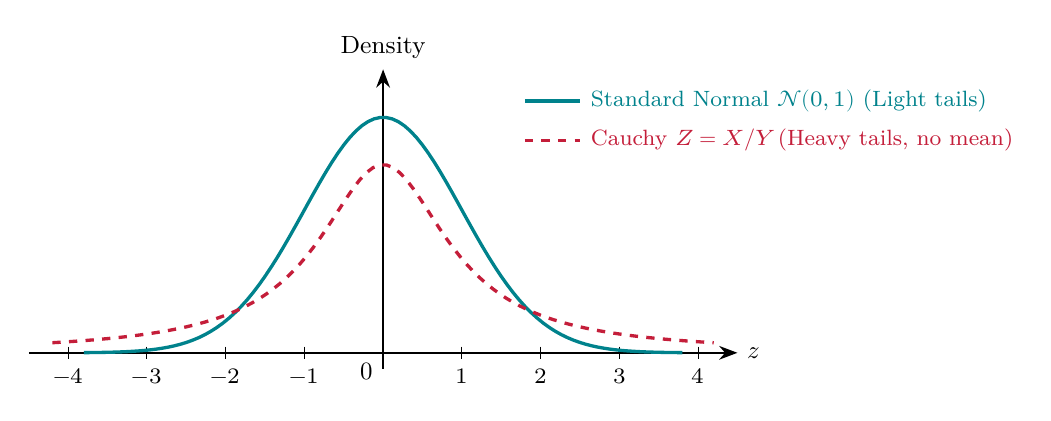
\begin{tikzpicture}[scale=1.0, every node/.style={font=\small}]
  % Axes
  \draw[-Stealth, thick] (-4.5, 0) -- (4.5, 0) node[right] {$z$};
  \draw[-Stealth, thick] (0, -0.2) -- (0, 3.6) node[above] {Density};

  % Ticks
  \foreach \x in {-4,-3,-2,-1,1,2,3,4} {
    \draw (\x, 0.08) -- (\x, -0.08) node[below] {\footnotesize $\x$};
  }
  \node[below left] at (0, 0) {$0$};

  % Standard Normal: peak 0.3989 -> scale * 7.5 = 2.99
  \draw[very thick, color=myteal, domain=-3.8:3.8, samples=100]
    plot (\x, {2.99*exp(-(\x)^2/2)});

  % Cauchy: f(z) = 1/(pi*(1+z^2)), peak at z=0 is 1/pi = 0.3183 -> scale * 7.5 = 2.39
  \draw[very thick, color=myred, dashed, domain=-4.2:4.2, samples=100]
    plot (\x, {2.39 / (1 + (\x)^2)});

  % Legend
  \draw[very thick, color=myteal] (1.8, 3.2) -- (2.5, 3.2) node[right, font=\footnotesize] {Standard Normal $\mathcal{N}(0, 1)$ (Light tails)};
  \draw[very thick, color=myred, dashed] (1.8, 2.7) -- (2.5, 2.7) node[right, font=\footnotesize] {Cauchy $Z = X/Y$ (Heavy tails, no mean)};
\end{tikzpicture}
\end{center}
\end{tcolorbox}

\newpage
% ===============================================================================
% MANDATORY QUICK REVISION PAGE
% ===============================================================================
\begin{center}
  {\large\bfseries\color{myred} Quick Revision --- Module 3}\\[1pt]
  {\small\color{mydark} Bivariate Distributions, Sums, Quotients and Bayes' Rule $|$ BS-M301}
\end{center}
\noindent{\color{myred}\rule{\linewidth}{1.0pt}}
\vspace{1pt}

\begin{tcolorbox}[formulabox, top=3pt, bottom=3pt, title={\textbf{Key Formulas and Bivariate Relations at a Glance}}]
\renewcommand{\arraystretch}{1.18}
\setlength{\tabcolsep}{4pt}
\begin{tabularx}{\linewidth}{B{3.4cm} X}
Joint PDF \& CDF & $f_{XY}(x,y) \ge 0, \; \iint f_{XY} dx dy = 1; \quad f_{XY}(x,y) = \frac{\partial^2 F_{XY}}{\partial x \partial y}$ \\[2.5pt]
Marginal Densities & $f_X(x) = \int_{-\infty}^\infty f_{XY}(x,y) dy, \quad f_Y(y) = \int_{-\infty}^\infty f_{XY}(x,y) dx$ \\[2.5pt]
Conditional Densities & $f_{X|Y}(x \mid y) = \frac{f_{XY}(x,y)}{f_Y(y)}, \quad f_{Y|X}(y \mid x) = \frac{f_{XY}(x,y)}{f_X(x)}$ \\[2.5pt]
Statistical Independence & $f_{XY}(x,y) = f_X(x) f_Y(y) \iff f_{X|Y}(x \mid y) = f_X(x)$ \\[2.5pt]
Tower Property & $E\left[E[X \mid Y]\right] = E[X], \quad \operatorname{Var}(X) = E[\operatorname{Var}(X|Y)] + \operatorname{Var}(E[X|Y])$ \\[2.5pt]
Jacobian Transform & $f_{UV}(u,v) = f_{XY}(h_1, h_2) \cdot |J|, \quad J = \det \begin{pmatrix} \frac{\partial x}{\partial u} & \frac{\partial x}{\partial v} \\ \frac{\partial y}{\partial u} & \frac{\partial y}{\partial v} \end{pmatrix}$ \\[2.5pt]
Sum \& Quotient PDFs & $Z = X+Y \implies f_Z = \int f(w, z-w) dw; \quad Z = \frac{X}{Y} \implies f_Z = \int |w| f(zw, w) dw$ \\[2.5pt]
Cauchy \& Bayes' Rule & $Z = \frac{X}{Y} \sim \text{Cauchy}: f_Z(z) = \frac{1}{\pi(1+z^2)}; \quad f_{X|Y}(x \mid y) = \frac{f_X(x) f_{Y|X}(y \mid x)}{\int_{-\infty}^\infty f_X(u) f_{Y|X}(y \mid u) du}$ \\
\end{tabularx}
\end{tcolorbox}

\vspace{1pt}

\begin{tcolorbox}[defbox, top=2pt, bottom=2pt, title={\textbf{One-Line Definitions}}]
\small
\begin{itemize}[leftmargin=12pt, itemsep=-0.6pt, topsep=0pt, parsep=0pt]
  \item \textbf{Joint PDF $f_{XY}(x,y)$:} Surface whose double integral over any region $D$ equals $P((X,Y) \in D)$.
  \item \textbf{Marginal PDF:} Individual density of one component obtained by integrating out the other variable.
  \item \textbf{Conditional PDF:} Sliced cross-sectional density of $X$ normalized by $f_Y(y)$ under $Y=y$.
  \item \textbf{Statistical Independence:} Factorization $f_{XY}(x,y) = f_X(x) f_Y(y)$ across the entire domain.
  \item \textbf{Tower Property:} Fundamental law asserting that overall expectation equals $E[E[X \mid Y]]$.
  \item \textbf{Jacobian Determinant ($J$):} Local area transformation ratio $dx dy = |J| du dv$ relating coordinate spaces.
  \item \textbf{Convolution Theorem:} Integral operation yielding the PDF of the sum of independent RVs: $f_Z = f_X * f_Y$.
  \item \textbf{Quotient Distribution:} Density $f_Z(z) = \int |w| f(zw, w) dw$ describing the ratio of two RVs.
  \item \textbf{Cauchy Distribution:} Heavy-tailed distribution $f(z) = \frac{1}{\pi(1+z^2)}$ formed by $\mathcal{N}(0,1)/\mathcal{N}(0,1)$, lacking moments.
  \item \textbf{Posterior Density:} Updated density of an unknown parameter after incorporating observation $y$.
\end{itemize}
\end{tcolorbox}

\newpage

\begin{tcolorbox}[exambox, title={\textbf{Frequently Asked / Viva Questions (Part 1)}}]
\begin{enumerate}[topsep=0pt, label=\textbf{Q\arabic*.}, itemsep=3.2pt]
  \item \Q{State the necessary and sufficient conditions for two continuous random variables $X$ and $Y$ to be independent.}
  $X$ and $Y$ are independent if and only if their joint PDF factors into the product of their marginal PDFs everywhere: $f_{XY}(x, y) = f_X(x) f_Y(y)$ for all $(x, y) \in \mathbb{R}^2$, and the support region $D$ is a product of intervals (non-coupled boundaries).

  \item \Q{How is the joint PDF obtained from the joint Cumulative Distribution Function?}
  By mixed second-order partial differentiation: $f_{XY}(x, y) = \frac{\partial^2}{\partial x \partial y} F_{XY}(x, y)$, provided the second partial derivatives exist and are continuous.

  \item \Q{State and prove the Law of Iterated Expectations (Tower Property).}
  $E\left[E[X \mid Y]\right] = E[X]$. Proof: $E[E[X \mid Y]] = \int \left(\int x \frac{f(x,y)}{f_Y(y)} dx\right) f_Y(y) dy = \iint x f(x,y) dx dy = \int x f_X(x) dx = E[X]$.

  \item \Q{What is the physical significance of the Jacobian determinant in bivariate transformations?}
  The Jacobian determinant $J = \frac{\partial(x, y)}{\partial(u, v)}$ represents the local geometric dilation factor between the original and transformed coordinate planes, ensuring conservation of probability mass: $P(dx dy) = f_{XY}(x, y) dx dy = f_{XY}(h_1, h_2) |J| du dv = f_{UV}(u, v) du dv$.

  \item \Q{Derive the PDF of the sum $Z = X + Y$ of two independent continuous random variables.}
  Let $Z = X + Y, W = X \implies X = W, Y = Z - W$. The Jacobian is $|J| = 1$. The joint density is $f_{ZW}(z, w) = f_{XY}(w, z - w) = f_X(w) f_Y(z - w)$. Integrating over $w$ gives the convolution: $f_Z(z) = \int_{-\infty}^\infty f_X(w) f_Y(z - w) dw$.

  \item \Q{Why does the absolute value $|w|$ appear in the formula for the quotient density $Z = X/Y$?}
  The Jacobian of the inverse transformation $x = z w, y = w$ is $J = \det \begin{pmatrix} w & z \\ 0 & 1 \end{pmatrix} = w$. Because an area element must always be strictly non-negative ($dx dy = |J| dz dw$), the absolute value $|J| = |w|$ must be taken.

  \item \Q{Show that the ratio of two independent standard normal random variables follows a Cauchy distribution.}
  $f_Z(z) = \frac{1}{2\pi} \int_{-\infty}^\infty |w| e^{-w^2(1+z^2)/2} dw = \frac{1}{\pi} \int_0^\infty w e^{-w^2(1+z^2)/2} dw$. Substituting $u = w^2(1+z^2)/2$ transforms the integral to $\frac{1}{\pi(1+z^2)} \int_0^\infty e^{-u} du = \frac{1}{\pi(1+z^2)}$, which is the standard Cauchy PDF.
\end{enumerate}
\end{tcolorbox}

\newpage

\begin{tcolorbox}[exambox, top=3pt, bottom=3pt, title={\textbf{Frequently Asked / Viva Questions (Part 2)}}]
\begin{enumerate}[topsep=0pt, label=\textbf{Q\arabic*.}, itemsep=1.8pt, start=8]
  \item \Q{Why does the Cauchy distribution have no mathematical expectation or variance?}
  $E[|Z|] = \frac{1}{\pi} \int_{-\infty}^\infty \frac{|z|}{1+z^2} dz = \frac{2}{\pi} \int_0^\infty \frac{z}{1+z^2} dz = \frac{1}{\pi} \left[\ln(1+z^2)\right]_0^\infty = \infty$. Because the absolute integral diverges logarithmically due to heavy polynomial tails ($\sim 1/z^2$), the mean is mathematically undefined, and all higher moments diverge.

  \item \Q{State the Law of Total Variance (Eve's Law) and interpret its terms.}
  $\operatorname{Var}(X) = E[\operatorname{Var}(X \mid Y)] + \operatorname{Var}(E[X \mid Y])$. The first term represents the average unexplained variation remaining in $X$ after conditioning on $Y$; the second term represents the variation in the conditional predictor $E[X \mid Y]$ explained by $Y$.

  \item \Q{State Continuous Bayes' Theorem and explain its role in signal estimation.}
  $f_{X|Y}(x \mid y) = \frac{f_X(x) f_{Y|X}(y \mid x)}{\int f_X(u) f_{Y|X}(y \mid u) du}$. In communications, $X$ is the transmitted signal (prior), $f_{Y|X}(y \mid x)$ is the channel noise model (likelihood), and $f_{X|Y}(x \mid y)$ is the posterior distribution used by the receiver to make Maximum A Posteriori (MAP) symbol decisions.
\end{enumerate}
\end{tcolorbox}

\vspace{2pt}

\begin{tcolorbox}[tikzbox, top=3pt, bottom=3pt, title={\textbf{Summary Matrix: Comprehensive Comparison of Bivariate Operations}}]
\par\vspace{1pt}\noindent
\begingroup
\setlength{\tabcolsep}{3.5pt}
\setlength{\extrarowheight}{1.0pt}
\renewcommand{\arraystretch}{1.15}
\begin{tabularx}{\linewidth}{|>{\small\bfseries\raggedright\arraybackslash}m{2.3cm}|>{\small\raggedright\arraybackslash}m{4.6cm}|>{\small\raggedright\arraybackslash}m{3.9cm}|Y|}
\hline
\textbf{Operation / Concept} & \textbf{Mathematical Governing Expression} & \textbf{Independence Simplification} & \textbf{Physical Meaning / Role} \\
\hline
Marginal Density & $f_X(x) = \int_{-\infty}^\infty f_{XY}(x, y) \, dy$ & $f_X(x) \int f_Y(y) dy = f_X(x)$ & Complete projection onto $X$-axis. \\
\hline
Conditional Density & $f_{X|Y}(x \mid y) = \frac{f_{XY}(x, y)}{f_Y(y)}$ & $f_{X|Y}(x \mid y) = f_X(x)$ & Updated density given knowledge $Y=y$. \\
\hline
Sum of RVs & $Z = X + Y \implies f_Z(z) = \int f_{XY}(w, z-w) dw$ & Convolution: $f_Z = f_X * f_Y$ & Total noise from independent sources. \\
\hline
Quotient of RVs & $Z = X / Y \implies f_Z(z) = \int |w| f_{XY}(zw, w) dw$ & $\int |w| f_X(zw) f_Y(w) dw$ & Signal-to-noise ratio; slope of vector. \\
\hline
Cauchy Ratio & $Z = X/Y$ for $X,Y \sim \mathcal{N}(0, 1) \implies \frac{1}{\pi(1+z^2)}$ & Quotient of two standard Gaussians & Heavy-tailed ratio; undefined moments. \\
\hline
Continuous Bayes & $f_{X|Y}(x \mid y) = \frac{f_X(x) f_{Y|X}(y \mid x)}{\int f_X(u) f_{Y|X}(y \mid u) du}$ & $f_{X|Y}(x \mid y) = f_X(x)$ & Optimal Bayesian estimation / inference. \\
\hline
\end{tabularx}
\endgroup
\end{tcolorbox}


% -- Module 4 -----------------------------------------------------------------
\modulestart{4}{Measures of Central Tendency, Moments, Skewness and Kurtosis}

\section{Measures of Central Tendency, Moments, Skewness and Kurtosis}
% ───────────────────────────────────────────────────────────────────────────────

Descriptive statistics provides quantitative summaries describing the central clustering, dispersion, asymmetry, and peakedness of experimental datasets.

\begin{tcolorbox}[defbox, title={\textbf{Definition: Measures of Central Tendency}}]
\begin{enumerate}[leftmargin=*, itemsep=2pt, topsep=2pt]
  \item \textbf{Arithmetic Mean ($\bar{x}$):} The sum of all observations divided by sample size:
  \begin{equation}
    \bar{x} = \frac{1}{N} \sum_{i=1}^n f_i x_i, \qquad N = \sum_{i=1}^n f_i
  \end{equation}
  \textit{Key Properties:} (1) Algebraic sum of deviations is zero: $\sum f_i (x_i - \bar{x}) = 0$. (2) Sum of squared deviations is minimal about the mean: $\sum f_i (x_i - A)^2$ is minimum when $A = \bar{x}$.
  \item \textbf{Median ($M$):} The middle value partitioning the ordered dataset into two equal halves. For grouped data with median class $[L, L+h]$:
  \begin{equation}
    M = L + \frac{\frac{N}{2} - C}{f} \cdot h
  \end{equation}
  where $L$ is lower boundary, $C$ is cumulative frequency of preceding class, and $f$ is frequency.
  \item \textbf{Mode ($Z$):} The most frequently occurring value in the distribution:
  \begin{equation}
    Z = L + \frac{f_1 - f_0}{2f_1 - f_0 - f_2} \cdot h
  \end{equation}
  \textbf{Empirical Relationship for Moderately Skewed Distributions:}
  \begin{equation}
    \text{Mode} \approx 3 \times \text{Median} - 2 \times \text{Mean} \iff \text{Mean} - \text{Mode} \approx 3(\text{Mean} - \text{Median})
  \end{equation}
\end{enumerate}
\end{tcolorbox}

\subsection{Moments and Moment Conversion Relations}
\begin{itemize}[leftmargin=*, itemsep=3pt]
  \item \textbf{$r$-th Raw Moment about Origin ($\mu_r'$):} $\mu_r' = \frac{1}{N} \sum f_i x_i^r$. Note: $\mu_1' = \bar{x}$.
  \item \textbf{$r$-th Central Moment about Mean ($\mu_r$):} $\mu_r = \frac{1}{N} \sum f_i (x_i - \bar{x})^r$.
\end{itemize}

\begin{tcolorbox}[formulabox, title={\textbf{Conversion Relations: Central Moments from Raw Moments}}]
Expanding $(x_i - \bar{x})^r = \sum_{k=0}^r \binom{r}{k} x_i^{r-k} (-\bar{x})^k$:
\begin{align}
  \mu_1 &= 0 \quad (\text{Always zero!}) \\[3pt]
  \mu_2 &= \mu_2' - (\mu_1')^2 = \sigma^2 \quad (\text{Variance}) \\[3pt]
  \mu_3 &= \mu_3' - 3\mu_2'\mu_1' + 2(\mu_1')^3 \\[3pt]
  \mu_4 &= \mu_4' - 4\mu_3'\mu_1' + 6\mu_2'(\mu_1')^2 - 3(\mu_1')^4
\end{align}
\end{tcolorbox}

\subsection{Measures of Skewness (Asymmetry)}
Skewness quantifies the departure of a distribution curve from perfect bilateral symmetry.
\begin{tcolorbox}[defbox, title={\textbf{Formulas for Coefficients of Skewness}}]
\begin{enumerate}[leftmargin=*, itemsep=3pt]
  \item \textbf{Karl Pearson's Coefficient of Skewness ($S_k$):}
  \begin{equation}
    S_k = \frac{\text{Mean} - \text{Mode}}{\sigma} = \frac{3(\text{Mean} - \text{Median})}{\sigma}, \qquad -3 \le S_k \le 3
  \end{equation}
  \item \textbf{Bowley's Quartile Coefficient of Skewness ($S_b$):} Based on quartiles $Q_1, Q_2 (\text{Median}), Q_3$:
  \begin{equation}
    S_b = \frac{(Q_3 - Q_2) - (Q_2 - Q_1)}{(Q_3 - Q_2) + (Q_2 - Q_1)} = \frac{Q_3 + Q_1 - 2Q_2}{Q_3 - Q_1}, \qquad -1 \le S_b \le 1
  \end{equation}
  \item \textbf{Moment Coefficient of Skewness ($\beta_1$ and $\gamma_1$):}
  \begin{equation}
    \beta_1 = \frac{\mu_3^2}{\mu_2^3} = \frac{\mu_3^2}{\sigma^6}, \qquad \gamma_1 = \sqrt{\beta_1} = \frac{\mu_3}{\sigma^3}
  \end{equation}
  \begin{itemize}[leftmargin=*, itemsep=1pt]
    \item $\gamma_1 = 0$: Symmetric distribution ($\text{Mean} = \text{Median} = \text{Mode}$).
    \item $\gamma_1 > 0$: Positively skewed (long tail stretched to the right; $\text{Mean} > \text{Median} > \text{Mode}$).
    \item $\gamma_1 < 0$: Negatively skewed (long tail stretched to the left; $\text{Mode} > \text{Median} > \text{Mean}$).
  \end{itemize}
\end{enumerate}
\end{tcolorbox}

\begin{tcolorbox}[tikzbox, title={\textbf{TikZ Schematic: Geometric Comparison of Symmetrical and Skewed Distributions}}]
\begin{center}
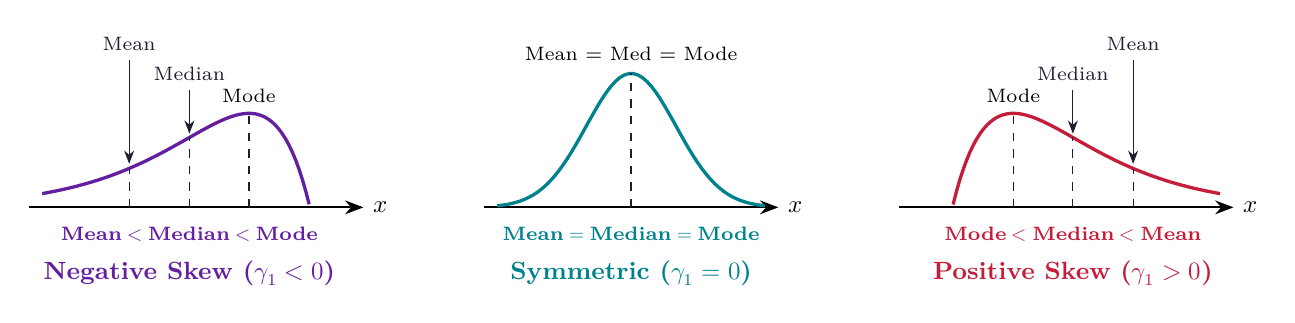
\begin{tikzpicture}[scale=0.85, every node/.style={font=\small}]
  % Symmetrical (Center)
  \begin{scope}[shift={(0,0)}]
    \draw[-Stealth, thick] (-2.2,0) -- (2.2,0) node[right] {$x$};
    \draw[very thick, color=myteal, domain=-2:2, samples=60] plot (\x, {2.0*exp(-(\x)^2/0.9)});
    \draw[dashed, thick, color=mydark] (0,0) -- (0,2.0);
    \node[above, font=\scriptsize] at (0,2.05) {Mean = Med = Mode};
    \node[below, font=\scriptsize\bfseries, color=myteal] at (0,-0.15) {$\text{Mean} = \text{Median} = \text{Mode}$};
    \node[below, font=\small\bfseries, color=myteal] at (0,-0.65) {Symmetric ($\gamma_1 = 0$)};
  \end{scope}

  % Positively Skewed (Right)
  \begin{scope}[shift={(4.8,0)}]
    \draw[-Stealth, thick] (-0.8,0) -- (4.2,0) node[right] {$x$};
    \draw[very thick, color=myred, domain=0.01:4.0, samples=80] plot (\x, {4.2*\x*exp(-1.1*\x)});
    \draw[dashed, thin, color=mydark] (0.91,0) -- (0.91,1.42);
    \node[above, font=\scriptsize] at (0.91,1.42) {Mode};
    \draw[dashed, thin, color=mydark] (1.8,0) -- (1.8,1.05);
    \draw[-Stealth, thin, color=mydark] (1.8,1.75) node[above, font=\scriptsize] {Median} -- (1.8,1.1);
    \draw[dashed, thin, color=mydark] (2.7,0) -- (2.7,0.58);
    \draw[-Stealth, thin, color=mydark] (2.7,2.2) node[above, font=\scriptsize] {Mean} -- (2.7,0.65);
    \node[below, font=\scriptsize\bfseries, color=myred] at (1.8,-0.15) {$\text{Mode} < \text{Median} < \text{Mean}$};
    \node[below, font=\small\bfseries, color=myred] at (1.8,-0.65) {Positive Skew ($\gamma_1 > 0$)};
  \end{scope}

  % Negatively Skewed (Left)
  \begin{scope}[shift={(-4.8,0)}]
    \draw[-Stealth, thick] (-4.2,0) -- (0.8,0) node[right] {$x$};
    \draw[very thick, color=mypurple, domain=-4.0:-0.01, samples=80] plot (\x, {-4.2*\x*exp(1.1*\x)});
    \draw[dashed, thin, color=mydark] (-2.7,0) -- (-2.7,0.58);
    \draw[-Stealth, thin, color=mydark] (-2.7,2.2) node[above, font=\scriptsize] {Mean} -- (-2.7,0.65);
    \draw[dashed, thin, color=mydark] (-1.8,0) -- (-1.8,1.05);
    \draw[-Stealth, thin, color=mydark] (-1.8,1.75) node[above, font=\scriptsize] {Median} -- (-1.8,1.1);
    \draw[dashed, thin, color=mydark] (-0.91,0) -- (-0.91,1.42);
    \node[above, font=\scriptsize] at (-0.91,1.42) {Mode};
    \node[below, font=\scriptsize\bfseries, color=mypurple] at (-1.8,-0.15) {$\text{Mean} < \text{Median} < \text{Mode}$};
    \node[below, font=\small\bfseries, color=mypurple] at (-1.8,-0.65) {Negative Skew ($\gamma_1 < 0$)};
  \end{scope}
\end{tikzpicture}
\end{center}
\end{tcolorbox}

\subsection{Measures of Kurtosis (Peakedness)}
\begin{tcolorbox}[defbox, title={\textbf{Definition: Kurtosis Coefficients $\beta_2$ and $\gamma_2$}}]
Kurtosis quantifies the degree of peakedness and the heaviness of the tails of a frequency curve relative to the standard normal bell curve:
\begin{equation}
  \beta_2 = \frac{\mu_4}{\mu_2^2} = \frac{\mu_4}{\sigma^4}, \qquad \gamma_2 = \beta_2 - 3
\end{equation}
\begin{itemize}[leftmargin=*, itemsep=2pt]
  \item \textbf{Mesokurtic ($\beta_2 = 3, \gamma_2 = 0$):} Normal distribution curve profile.
  \item \textbf{Leptokurtic ($\beta_2 > 3, \gamma_2 > 0$):} Sharply peaked center with heavy, fat tails (e.g., Student's $t$, Laplace).
  \item \textbf{Platykurtic ($\beta_2 < 3, \gamma_2 < 0$):} Flatter plateau-like peak with light, rapidly vanishing tails (e.g., Uniform distribution where $\beta_2 = 1.8$).
\end{itemize}
\end{tcolorbox}

% ───────────────────────────────────────────────────────────────────────────────
\section{Evaluation of Statistical Parameters for Core Distributions}
% ───────────────────────────────────────────────────────────────────────────────

\subsection{Binomial Distribution: Parameters and Recurrence Relation}
For $X \sim \text{Bin}(n, p)$ with $q = 1-p$:
\begin{equation}
  M_X(t) = \sum_{k=0}^n e^{tk} \binom{n}{k} p^k q^{n-k} = (q + p e^t)^n
\end{equation}
\begin{align}
  E[X] &= \mu = np, \qquad \operatorname{Var}(X) = \sigma^2 = npq \\[3pt]
  \mu_3 &= npq(q - p), \qquad \mu_4 = 3n^2 p^2 q^2 + npq(1 - 6pq) \\[3pt]
  \beta_1 &= \frac{\mu_3^2}{\mu_2^3} = \frac{(q-p)^2}{npq}, \qquad \beta_2 = \frac{\mu_4}{\mu_2^2} = 3 + \frac{1 - 6pq}{npq}
\end{align}
\textit{Recurrence Relation for Central Moments:}
\begin{equation}
  \mu_{r+1} = pq \left[n r \mu_{r-1} + \frac{d\mu_r}{dp}\right]
\end{equation}

\subsection{Poisson Distribution: Parameters and Recurrence Relation}
For $X \sim \text{Poisson}(\lambda)$:
\begin{equation}
  M_X(t) = \sum_{k=0}^\infty e^{tk} \frac{\lambda^k e^{-\lambda}}{k!} = e^{-\lambda} \sum_{k=0}^\infty \frac{(\lambda e^t)^k}{k!} = e^{-\lambda} e^{\lambda e^t} = \exp\left(\lambda(e^t - 1)\right)
\end{equation}
\begin{align}
  E[X] &= \lambda, \qquad \operatorname{Var}(X) = \lambda \\[3pt]
  \mu_3 &= \lambda, \qquad \mu_4 = 3\lambda^2 + \lambda \\[3pt]
  \beta_1 &= \frac{\mu_3^2}{\mu_2^3} = \frac{\lambda^2}{\lambda^3} = \frac{1}{\lambda}, \qquad \beta_2 = \frac{3\lambda^2 + \lambda}{\lambda^2} = 3 + \frac{1}{\lambda}
\end{align}
\textit{Recurrence Relation for Central Moments:}
\begin{equation}
  \mu_{r+1} = \lambda \left[r \mu_{r-1} + \frac{d\mu_r}{d\lambda}\right]
\end{equation}
As $\lambda \to \infty$, both $\beta_1 \to 0$ and $\beta_2 \to 3$, confirming convergence of Poisson to Normal!

\subsection{Normal Distribution: Parameters and Recurrence Relation}
For $X \sim \mathcal{N}(\mu, \sigma^2)$:
\begin{align}
  E[X] &= \mu, \qquad \operatorname{Var}(X) = \sigma^2 \\[3pt]
  \mu_{2k+1} &= 0 \quad \forall k \in \mathbb{N}_0, \qquad \mu_{2k} = \frac{(2k)!}{2^k k!} \sigma^{2k} \\[3pt]
  \beta_1 &= 0, \qquad \beta_2 = \frac{3\sigma^4}{\sigma^4} = 3 \iff \gamma_2 = 0
\end{align}
\textit{Recurrence Relation for Even Central Moments:}
\begin{equation}
  \mu_{2k} = (2k - 1) \sigma^2 \mu_{2k-2}
\end{equation}

% ───────────────────────────────────────────────────────────────────────────────
\section{Correlation and Regression Analysis}
% ───────────────────────────────────────────────────────────────────────────────

\subsection{Karl Pearson's Coefficient of Correlation ($r$)}
Karl Pearson's product-moment correlation coefficient $r$ provides a scale-invariant measure of linear association between two paired variables $(x_i, y_i)$:
\begin{tcolorbox}[formulabox, title={\textbf{Formula for Pearson's Correlation Coefficient}}]
\begin{equation}
  r = \frac{\operatorname{Cov}(X, Y)}{\sigma_x \sigma_y} = \frac{\displaystyle\sum_{i=1}^n (x_i - \bar{x})(y_i - \bar{y})}{\sqrt{\displaystyle\sum_{i=1}^n (x_i - \bar{x})^2} \sqrt{\displaystyle\sum_{i=1}^n (y_i - \bar{y})^2}} = \frac{n \sum x_i y_i - (\sum x_i)(\sum y_i)}{\sqrt{n\sum x_i^2 - (\sum x_i)^2}\sqrt{n\sum y_i^2 - (\sum y_i)^2}}
\end{equation}
\textbf{Properties of $r$:}
\begin{enumerate}[leftmargin=*, itemsep=2pt]
  \item Normalized limits: $-1 \le r \le +1$.
  \item Invariant to change of origin and scale: If $u = \frac{x - a}{h}$ and $v = \frac{y - b}{k}$ with $h, k > 0$, then $r_{xy} = r_{uv}$.
\end{enumerate}
\end{tcolorbox}

\subsection{Linear Regression Equations and Least Squares}
Regression expresses the average functional relationship predicting a dependent variable from an independent variable.
\begin{tcolorbox}[defbox, title={\textbf{The Two Lines of Regression}}]
\textbf{1. Line of Regression of $Y$ on $X$:} Predicts $Y$ for a known value of $X$:
\begin{equation}
  Y - \bar{y} = b_{yx} (X - \bar{x}), \qquad b_{yx} = r \frac{\sigma_y}{\sigma_x} = \frac{\operatorname{Cov}(X, Y)}{\sigma_x^2}
\end{equation}
\textbf{2. Line of Regression of $X$ on $Y$:} Predicts $X$ for a known value of $Y$:
\begin{equation}
  X - \bar{x} = b_{xy} (Y - \bar{y}), \qquad b_{xy} = r \frac{\sigma_x}{\sigma_y} = \frac{\operatorname{Cov}(X, Y)}{\sigma_y^2}
\end{equation}
where $b_{yx}$ and $b_{xy}$ are the \textbf{regression coefficients}.
\end{tcolorbox}

\begin{tcolorbox}[formulabox, title={\textbf{Key Properties of Regression Coefficients}}]
\begin{enumerate}[leftmargin=*, itemsep=3pt]
  \item \textbf{Geometric Mean Property:} The correlation coefficient is the geometric mean of the regression coefficients:
  \begin{equation}
    r = \pm \sqrt{b_{yx} \cdot b_{xy}}
  \end{equation}
  Both regression coefficients must share the same algebraic sign, which is also the sign of $r$.
  \item \textbf{Reciprocal Magnitude Constraint:} If $b_{yx} > 1$, then $b_{xy} < 1$, since $b_{yx} b_{xy} = r^2 \le 1$.
  \item \textbf{Arithmetic Mean Inequality:} $\dfrac{b_{yx} + b_{xy}}{2} \ge r$ (by AM $\ge$ GM).
  \item \textbf{Centroid Intersection:} Both lines intersect at the point of means $(\bar{x}, \bar{y})$.
  \item \textbf{Scale Dependence:} Regression coefficients are invariant to change of origin, but \textbf{depend} on scale: $b_{yx} = \frac{k}{h} b_{vu}$.
\end{enumerate}
\end{tcolorbox}

\subsection{Angle Between the Two Regression Lines}
\begin{tcolorbox}[examplebox, title={\textbf{Derivation: Angle $\theta$ Between Regression Lines}}]
The slopes of the two lines in the $(X, Y)$ plane are:
\begin{equation}
  m_1 = b_{yx} = r \frac{\sigma_y}{\sigma_x}, \qquad m_2 = \frac{1}{b_{xy}} = \frac{\sigma_y}{r \sigma_x}
\end{equation}
The angle $\theta$ between the lines satisfies:
\begin{equation}
  \tan\theta = \left|\frac{m_2 - m_1}{1 + m_1 m_2}\right| = \left|\frac{\frac{\sigma_y}{r\sigma_x} - r\frac{\sigma_y}{\sigma_x}}{1 + \left(r\frac{\sigma_y}{\sigma_x}\right)\left(\frac{\sigma_y}{r\sigma_x}\right)}\right| = \left|\frac{\frac{\sigma_y}{\sigma_x}\left(\frac{1 - r^2}{r}\right)}{1 + \frac{\sigma_y^2}{\sigma_x^2}}\right|
\end{equation}
Simplifying the denominator $1 + \sigma_y^2/\sigma_x^2 = (\sigma_x^2 + \sigma_y^2)/\sigma_x^2$:
\begin{equation}
  \tan\theta = \left(\frac{1 - r^2}{|r|}\right) \left(\frac{\sigma_x \sigma_y}{\sigma_x^2 + \sigma_y^2}\right)
\end{equation}
\textbf{Special Cases:}
\begin{itemize}[leftmargin=*, itemsep=2pt]
  \item If $r = \pm 1 \implies \tan\theta = 0 \implies \theta = 0^\circ$ (the two lines \textbf{coincide}; perfect linear correlation).
  \item If $r = 0 \implies \tan\theta \to \infty \implies \theta = 90^\circ$ (the two lines are \textbf{perpendicular} parallel to coordinate axes; uncorrelated).
\end{itemize}
\end{tcolorbox}

\begin{tcolorbox}[tikzbox, title={\textbf{TikZ Plot: Scatter Diagram and the Two Lines of Regression with Intersection at Centroid}}]
\begin{center}
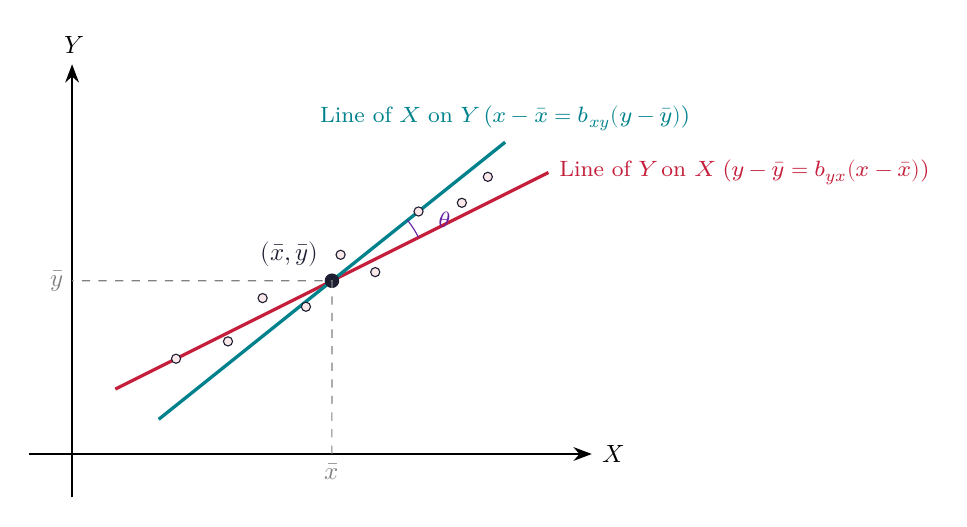
\begin{tikzpicture}[scale=1.1, every node/.style={font=\small}]
  % Axes
  \draw[-Stealth, thick] (-0.5, 0) -- (6.0, 0) node[right] {$X$};
  \draw[-Stealth, thick] (0, -0.5) -- (0, 4.5) node[above] {$Y$};

  % Centroid point (x_bar, y_bar) = (3, 2)
  \coordinate (C) at (3.0, 2.0);

  % Line of Y on X: y - 2 = 0.5(x - 3) -> slope 0.5
  \draw[very thick, color=myred] (0.5, 0.75) -- (5.5, 3.25)
    node[right, font=\footnotesize] {Line of $Y$ on $X$ ($y - \bar{y} = b_{yx}(x - \bar{x})$)};

  % Line of X on Y: x - 3 = 1.25(y - 2) -> y - 2 = 0.8(x - 3) -> slope 0.8
  \draw[very thick, color=myteal] (1.0, 0.4) -- (5.0, 3.6)
    node[above, font=\footnotesize] {Line of $X$ on $Y$ ($x - \bar{x} = b_{xy}(y - \bar{y})$)};

  % Centroid marker
  \filldraw[color=mydark] (C) circle (2.2pt) node[above left=2pt] {$(\bar{x}, \bar{y})$};
  \draw[dashed, thin, color=gray] (3.0, 0) node[below] {$\bar{x}$} -- (C) -- (0, 2.0) node[left] {$\bar{y}$};

  % Angle arc between lines
  \draw[thin, color=mypurple] (4.0, 2.5) arc (26.5:38.6:1.12);
  \node[color=mypurple, font=\footnotesize] at (4.3, 2.7) {$\theta$};

  % Scatter sample points
  \foreach \p in {(1.2, 1.1), (1.8, 1.3), (2.2, 1.8), (2.7, 1.7), (3.1, 2.3), (3.5, 2.1), (4.0, 2.8), (4.5, 2.9), (4.8, 3.2)} {
    \filldraw[color=mydark, fill=hdrred] \p circle (1.5pt);
  }
\end{tikzpicture}
\end{center}
\end{tcolorbox}

\subsection{Spearman's Rank Correlation Coefficient ($r_s$)}
When variables represent qualitative attributes that cannot be measured numerically but can be ordered or ranked (e.g., beauty, intelligence, performance rankings):
\begin{tcolorbox}[defbox, title={\textbf{Spearman's Rank Correlation Formula}}]
Let $R_{xi}$ and $R_{yi}$ denote the ranks assigned to the $i$-th individual, with difference $d_i = R_{xi} - R_{yi}$.
\begin{enumerate}[leftmargin=*, itemsep=3pt]
  \item \textbf{Case 1: When Ranks are Distinct (No Ties):}
  \begin{equation}
    r_s = 1 - \frac{6 \displaystyle\sum_{i=1}^n d_i^2}{n(n^2 - 1)}
  \end{equation}
  \item \textbf{Case 2: When Ranks are Tied (Correction Factor):} If an attribute value repeats $m$ times, all tied entries are allocated the average rank, and a correction factor $\frac{m(m^2 - 1)}{12}$ is added for each tie group:
  \begin{equation}
    r_s = 1 - \frac{6 \left[\displaystyle\sum_{i=1}^n d_i^2 + \sum_{j} \frac{m_j(m_j^2 - 1)}{12}\right]}{n(n^2 - 1)}
  \end{equation}
\end{enumerate}
\end{tcolorbox}

\newpage
% ===============================================================================
% MANDATORY QUICK REVISION PAGE
% ===============================================================================
\begin{center}
  {\large\bfseries\color{myred} Quick Revision --- Module 4}\\[1pt]
  {\small\color{mydark} Basic Statistics, Moments, Distributions, Correlation and Regression $|$ BS-M301}
\end{center}
\noindent{\color{myred}\rule{\linewidth}{1.0pt}}
\vspace{1pt}

\begin{tcolorbox}[formulabox, top=2pt, bottom=2pt, title={\textbf{Key Formulas and Statistical Identities at a Glance}}]
\renewcommand{\arraystretch}{0.96}
\setlength{\tabcolsep}{3.5pt}
\begin{tabularx}{\linewidth}{B{3.8cm} X}
Empirical Mean-Mode & $\text{Mode} \approx 3\text{Median} - 2\text{Mean} \iff \text{Mean}-\text{Mode} \approx 3(\text{Mean}-\text{Median})$ \\[0.2pt]
Central from Raw Moments & $\mu_2 = \mu_2'-(\mu_1')^2, \; \mu_3 = \mu_3'-3\mu_2'\mu_1'+2(\mu_1')^3, \; \mu_4 = \mu_4'-4\mu_3'\mu_1'+6\mu_2'(\mu_1')^2-3(\mu_1')^4$ \\[0.2pt]
Pearson Skewness & $S_k = \frac{\text{Mean}-\text{Mode}}{\sigma} = \frac{3(\text{Mean}-\text{Median})}{\sigma}, \quad \beta_1 = \frac{\mu_3^2}{\mu_2^3}, \quad \gamma_1 = \frac{\mu_3}{\sigma^3}$ \\[0.2pt]
Kurtosis Coefficients & $\beta_2 = \frac{\mu_4}{\mu_2^2} = \frac{\mu_4}{\sigma^4}, \quad \gamma_2 = \beta_2 - 3 \quad (\text{Meso}=3, \text{Lepto}>3, \text{Platy}<3)$ \\[0.2pt]
Binomial Parameters & $\mu = np, \quad \sigma^2 = npq, \quad \beta_1 = \frac{(q-p)^2}{npq}, \quad \beta_2 = 3 + \frac{1-6pq}{npq}$ \\[0.2pt]
Poisson Parameters & $\mu = \lambda, \quad \sigma^2 = \lambda, \quad \beta_1 = \frac{1}{\lambda}, \quad \beta_2 = 3 + \frac{1}{\lambda}$ \\[0.2pt]
Normal Moments & All odd $\mu_{2k+1}=0, \quad \mu_{2k} = \frac{(2k)!}{2^k k!} \sigma^{2k}, \quad \beta_1 = 0, \quad \beta_2 = 3$ \\[0.2pt]
Pearson Correlation & $r = \frac{\operatorname{Cov}(X,Y)}{\sigma_x \sigma_y} = \frac{\sum(x-\bar{x})(y-\bar{y})}{\sqrt{\sum(x-\bar{x})^2\sum(y-\bar{y})^2}} \in [-1, +1]$ \\[0.2pt]
Regression Lines & $Y-\bar{y} = b_{yx}(X-\bar{x}), \quad X-\bar{x} = b_{xy}(Y-\bar{y}), \quad b_{yx} = r\frac{\sigma_y}{\sigma_x}, \; b_{xy} = r\frac{\sigma_x}{\sigma_y}$ \\[0.2pt]
Regression Properties & $r = \pm\sqrt{b_{yx} b_{xy}}, \quad \frac{b_{yx}+b_{xy}}{2} \ge r, \quad \tan\theta = \frac{1-r^2}{|r|}\frac{\sigma_x \sigma_y}{\sigma_x^2+\sigma_y^2}$ \\[0.2pt]
Spearman Rank Corr. & $r_s = 1 - \frac{6\sum d_i^2}{n(n^2-1)} \quad (\text{Ties add } \sum\frac{m_j(m_j^2-1)}{12})$ \\
\end{tabularx}
\end{tcolorbox}

\vspace{1pt}

\begin{tcolorbox}[defbox, top=2pt, bottom=2pt, title={\textbf{One-Line Definitions}}]
\begin{itemize}[leftmargin=*, itemsep=-0.5pt, topsep=0pt, parsep=0pt]
  \item \textbf{Arithmetic Mean:} Center of gravity of data where algebraic sum of deviations $\sum(x_i - \bar{x})$ is identically zero.
  \item \textbf{Median \& Mode:} Median is positional 50th percentile; Mode is observation exhibiting peak frequency density.
  \item \textbf{Skewness:} Metric quantifying directional asymmetry of frequency curve tail relative to central peak.
  \item \textbf{Kurtosis:} Measure of peakedness and tail fatness relative to standard Gaussian benchmark ($\beta_2 = 3$).
  \item \textbf{Leptokurtic Curve:} Sharply peaked frequency profile with fat heavy tails exhibiting $\beta_2 > 3$.
  \item \textbf{Platykurtic Curve:} Broad-shouldered flattened frequency curve with light rapidly decaying tails ($\beta_2 < 3$).
  \item \textbf{Pearson's $r$:} Standardized dimensionless measure of the strength and direction of linear association.
  \item \textbf{Regression Line:} Optimal line minimizing sum of squared vertical/horizontal prediction errors (Least Squares).
  \item \textbf{Regression Coefficients:} Directional slopes $b_{yx}$ and $b_{xy}$ whose geometric mean equals correlation coefficient $r$.
  \item \textbf{Spearman's Rank Correlation:} Non-parametric correlation measuring monotonic agreement between ordinal rankings.
\end{itemize}
\end{tcolorbox}

\newpage

\begin{tcolorbox}[exambox, title={\textbf{Frequently Asked / Viva Questions (Part 1)}}]
\begin{enumerate}[topsep=0pt, label=\textbf{Q\arabic*.}, itemsep=3.2pt]
  \item \Q{State the algebraic properties of the Arithmetic Mean.}
  (1) The sum of deviations of all observations from their arithmetic mean is zero: $\sum f_i (x_i - \bar{x}) = 0$. (2) The sum of squared deviations is minimal when taken about the mean: $\sum f_i (x_i - A)^2$ is minimum for $A = \bar{x}$. (3) Mean of combined series: $\bar{x}_{12} = \frac{n_1 \bar{x}_1 + n_2 \bar{x}_2}{n_1 + n_2}$.

  \item \Q{Derive the relationship $\mu_3 = \mu_3' - 3\mu_2'\mu_1' + 2(\mu_1')^3$.}
  $\mu_3 = E[(X - \mu)^3] = E[X^3 - 3X^2\mu + 3X\mu^2 - \mu^3] = E[X^3] - 3\mu E[X^2] + 3\mu^2 E[X] - \mu^3$. Substituting $E[X] = \mu_1', E[X^2] = \mu_2', E[X^3] = \mu_3'$: $\mu_3 = \mu_3' - 3\mu_1'\mu_2' + 3(\mu_1')^3 - (\mu_1')^3 = \mu_3' - 3\mu_2'\mu_1' + 2(\mu_1')^3$.

  \item \Q{Distinguish between positive skewness and negative skewness with sketches.}
  In positive skewness, the tail is extended to the right, and $\text{Mean} > \text{Median} > \text{Mode}$ ($\gamma_1 > 0$). In negative skewness, the tail is extended to the left, and $\text{Mode} > \text{Median} > \text{Mean}$ ($\gamma_1 < 0$).

  \item \Q{What are Leptokurtic, Mesokurtic and Platykurtic curves?}
  A curve with $\beta_2 = 3$ is Mesokurtic (Normal). If $\beta_2 > 3$, it is Leptokurtic (more peaked with heavier tails). If $\beta_2 < 3$, it is Platykurtic (flatter top with lighter tails).

  \item \Q{State the recurrence relation for central moments of a Poisson distribution.}
  $\mu_{r+1} = \lambda \left[r \mu_{r-1} + \frac{d\mu_r}{d\lambda}\right]$. For $r=1$: $\mu_2 = \lambda(1\cdot 0 + 1) = \lambda$. For $r=2$: $\mu_3 = \lambda(2\cdot 0 + \frac{d\lambda}{d\lambda}) = \lambda$. For $r=3$: $\mu_4 = \lambda(3\lambda + \frac{d\lambda}{d\lambda}) = 3\lambda^2 + \lambda$.

  \item \Q{Prove that the correlation coefficient is the geometric mean of the two regression coefficients.}
  $b_{yx} = r \frac{\sigma_y}{\sigma_x}$ and $b_{xy} = r \frac{\sigma_x}{\sigma_y}$. Multiplying: $b_{yx} \cdot b_{xy} = \left(r\frac{\sigma_y}{\sigma_x}\right)\left(r\frac{\sigma_x}{\sigma_y}\right) = r^2$. Taking the square root: $r = \pm \sqrt{b_{yx} \cdot b_{xy}}$.

  \item \Q{Can two regression coefficients be $1.5$ and $0.8$? Explain.}
  Yes! $b_{yx} \cdot b_{xy} = (1.5)(0.8) = 1.2 > 1$. But wait: $r^2 = b_{yx} b_{xy} \le 1$. Since $1.2 > 1$, this would imply $r^2 > 1$, which violates the Cauchy-Schwarz bound $|r| \le 1$. Hence $b_{yx}=1.5$ and $b_{xy}=0.8$ is impossible!
\end{enumerate}
\end{tcolorbox}

\newpage

\begin{tcolorbox}[exambox, top=3pt, bottom=3pt, title={\textbf{Frequently Asked / Viva Questions (Part 2)}}]
\begin{enumerate}[topsep=0pt, label=\textbf{Q\arabic*.}, itemsep=1.8pt, start=8]
  \item \Q{Why are there two lines of regression rather than a single line?}
  Because the regression of $Y$ on $X$ minimizes the sum of squared vertical errors $\sum (y_i - \hat{y}_i)^2$, whereas the regression of $X$ on $Y$ minimizes the sum of squared horizontal errors $\sum (x_i - \hat{x}_i)^2$. The two lines coincide if and only if $r = \pm 1$ (zero error).

  \item \Q{State the formula for the angle $\theta$ between the two regression lines and interpret the extreme cases.}
  $\tan\theta = \frac{1-r^2}{|r|}\frac{\sigma_x \sigma_y}{\sigma_x^2 + \sigma_y^2}$. If $r = \pm 1$, $\tan\theta = 0 \implies \theta = 0^\circ$ (lines coincide; perfect correlation). If $r = 0$, $\tan\theta = \infty \implies \theta = 90^\circ$ (lines are perpendicular; uncorrelated).

  \item \Q{Derive Spearman's Rank Correlation formula when ranks are not tied.}
  Let $x_i, y_i$ be ranks from $1$ to $n$. Then $\bar{x} = \bar{y} = \frac{n+1}{2}$, $\sigma_x^2 = \sigma_y^2 = \frac{n^2-1}{12}$. Since $d_i = x_i - y_i$, $\sum d_i^2 = \sum (x_i - \bar{x})^2 + \sum (y_i - \bar{y})^2 - 2\sum (x_i - \bar{x})(y_i - \bar{y}) = 2n\sigma_x^2 - 2n r \sigma_x^2 = 2n\sigma_x^2(1 - r_s)$. Substituting $\sigma_x^2 = \frac{n^2-1}{12}$ yields $r_s = 1 - \frac{6\sum d_i^2}{n(n^2-1)}$.
\end{enumerate}
\end{tcolorbox}

\vspace{2pt}

\begin{tcolorbox}[tikzbox, top=3pt, bottom=3pt, title={\textbf{Summary Matrix: Comparison of Binomial, Poisson and Normal Distributions}}]
\par\vspace{1pt}\noindent
\begingroup
\setlength{\tabcolsep}{3.5pt}
\setlength{\extrarowheight}{1.0pt}
\renewcommand{\arraystretch}{1.12}
\begin{tabularx}{\linewidth}{|B{2.5cm}|B{3.2cm}|B{2.2cm}|B{2.5cm}|Y|}
\hline
\textbf{Parameter} & \textbf{Binomial $\text{Bin}(n, p)$} & \textbf{Poisson $\text{Poisson}(\lambda)$} & \textbf{Normal $\mathcal{N}(\mu, \sigma^2)$} & \textbf{Comparative Property} \\
\hline
Mean ($E[X]$) & $np$ & $\lambda$ & $\mu$ & Location measure. \\
\hline
Variance ($\sigma^2$) & $npq < \mu$ & $\lambda = \mu$ & $\sigma^2$ (Independent of $\mu$) & $\text{Var}_{\text{Bin}} < \text{Mean}$; $\text{Var}_{\text{Poi}} = \text{Mean}$. \\
\hline
MGF ($M_X(t)$) & $(q + p e^t)^n$ & $\exp(\lambda(e^t - 1))$ & $\exp(\mu t + \frac{1}{2}\sigma^2 t^2)$ & Poisson is limiting Binomial MGF. \\
\hline
Skewness ($\gamma_1$) & $\frac{q - p}{\sqrt{npq}}$ & $\frac{1}{\sqrt{\lambda}}$ & $0$ & Binomial is symmetric if $p = 0.5$. \\
\hline
Kurtosis ($\beta_2$) & $3 + \frac{1 - 6pq}{npq}$ & $3 + \frac{1}{\lambda}$ & $3$ ($\gamma_2 = 0$) & Both converge to $3$ as $n, \lambda \to \infty$. \\
\hline
\end{tabularx}
\endgroup
\end{tcolorbox}


% -- Module 5 -----------------------------------------------------------------
\modulestart{5}{Curve Fitting by the Method of Least Squares}

\section{Curve Fitting by the Method of Least Squares}
% ───────────────────────────────────────────────────────────────────────────────

In experimental electronics and engineering measurement, observational data points $(x_1, y_1), (x_2, y_2), \dots, (x_n, y_n)$ rarely lie on an exact mathematical curve due to sensor noise and environmental fluctuations. The \textbf{Method of Least Squares} provides an objective criterion to establish the best-fitting functional relationship $y = f(x; a, b, c, \dots)$ by minimizing the sum of the squared vertical discrepancies.

\begin{tcolorbox}[defbox, title={\textbf{Definition: The Principle of Least Squares}}]
Let $(x_i, y_i)$ be $n$ paired experimental measurements. For any chosen curve $y = f(x)$, the residual (vertical error) for the $i$-th observation is:
\begin{equation}
  e_i = y_i - f(x_i)
\end{equation}
The Principle of Least Squares states that the optimal curve parameters are those that minimize the total sum of squared residuals:
\begin{equation}
  S = \sum_{i=1}^n e_i^2 = \sum_{i=1}^n \left[y_i - f(x_i; a, b, c, \dots)\right]^2 = \text{Minimum}
\end{equation}
To achieve this minimum, the partial derivatives of $S$ with respect to each undetermined parameter must vanish simultaneously:
\begin{equation}
  \frac{\partial S}{\partial a} = 0, \qquad \frac{\partial S}{\partial b} = 0, \qquad \frac{\partial S}{\partial c} = 0, \quad \dots
\end{equation}
The resulting system of simultaneous equations is called the \textbf{Normal Equations}.
\end{tcolorbox}

\begin{tcolorbox}[tikzbox, title={\textbf{TikZ Schematic: Residual Errors and Best-Fit Curve in Least Squares}}]
\begin{center}
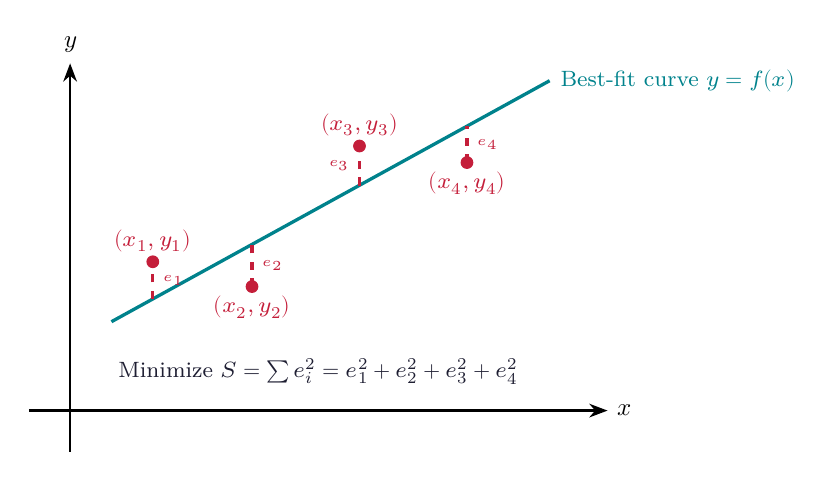
\begin{tikzpicture}[scale=1.05, every node/.style={font=\small}]
  % Axes
  \draw[-Stealth, thick] (-0.5, 0) -- (6.5, 0) node[right] {$x$};
  \draw[-Stealth, thick] (0, -0.5) -- (0, 4.2) node[above] {$y$};

  % Best fit line y = 0.55x + 0.8
  \draw[very thick, color=myteal] (0.5, 1.075) -- (5.8, 3.99) node[right, font=\footnotesize] {Best-fit curve $y = f(x)$};

  % Sample data points and vertical residuals
  % p1 = (1.0, 1.8), line = 1.35, e1 = +0.45
  \filldraw[color=myred] (1.0, 1.8) circle (2pt) node[above, font=\footnotesize] {$(x_1, y_1)$};
  \draw[dashed, very thick, color=myred] (1.0, 1.35) -- (1.0, 1.8) node[midway, right, font=\tiny] {$e_1$};

  % p2 = (2.2, 1.5), line = 2.01, e2 = -0.51
  \filldraw[color=myred] (2.2, 1.5) circle (2pt) node[below, font=\footnotesize] {$(x_2, y_2)$};
  \draw[dashed, very thick, color=myred] (2.2, 1.5) -- (2.2, 2.01) node[midway, right, font=\tiny] {$e_2$};

  % p3 = (3.5, 3.2), line = 2.72, e3 = +0.48
  \filldraw[color=myred] (3.5, 3.2) circle (2pt) node[above, font=\footnotesize] {$(x_3, y_3)$};
  \draw[dashed, very thick, color=myred] (3.5, 2.72) -- (3.5, 3.2) node[midway, left, font=\tiny] {$e_3$};

  % p4 = (4.8, 3.0), line = 3.44, e4 = -0.44
  \filldraw[color=myred] (4.8, 3.0) circle (2pt) node[below, font=\footnotesize] {$(x_4, y_4)$};
  \draw[dashed, very thick, color=myred] (4.8, 3.0) -- (4.8, 3.44) node[midway, right, font=\tiny] {$e_4$};

  % Caption
  \node[above, color=mydark, font=\footnotesize] at (3.0, 0.2) {Minimize $S = \sum e_i^2 = e_1^2 + e_2^2 + e_3^2 + e_4^2$};
\end{tikzpicture}
\end{center}
\end{tcolorbox}

\subsection{1. Fitting of a Straight Line: $y = a + bx$}
\begin{tcolorbox}[examplebox, title={\textbf{Derivation of Normal Equations for a Straight Line}}]
Let the straight line equation be $y = a + bx$. The error sum of squares is:
\begin{equation}
  S = \sum_{i=1}^n (y_i - a - bx_i)^2
\end{equation}
Differentiating partially with respect to $a$ and equating to zero:
\begin{align}
  \frac{\partial S}{\partial a} &= \sum_{i=1}^n 2(y_i - a - bx_i)(-1) = 0 \implies \sum_{i=1}^n (y_i - a - bx_i) = 0 \nonumber \\[3pt]
                                &\implies \sum y = n a + b \sum x
\end{align}
Differentiating partially with respect to $b$ and equating to zero:
\begin{align}
  \frac{\partial S}{\partial b} &= \sum_{i=1}^n 2(y_i - a - bx_i)(-x_i) = 0 \implies \sum_{i=1}^n x_i (y_i - a - bx_i) = 0 \nonumber \\[3pt]
                                &\implies \sum x y = a \sum x + b \sum x^2
\end{align}
\textbf{The Normal Equations for a Straight Line:}
\begin{align}
  \sum y &= n a + b \sum x \\[3pt]
  \sum x y &= a \sum x + b \sum x^2
\end{align}
\textit{Computation Shortcut (Change of Origin):} If $n$ is odd and values of $x$ are equally spaced, choosing the origin at the midpoint such that $\sum u = 0$ simplifies the solution to:
\begin{equation}
  a = \frac{\sum y}{n}, \qquad b = \frac{\sum u y}{\sum u^2}
\end{equation}
\end{tcolorbox}

\subsection{2. Fitting of a Second-Degree Parabola: $y = a + bx + cx^2$}
\begin{tcolorbox}[formulabox, title={\textbf{Normal Equations for a Second-Degree Parabola}}]
For the quadratic curve $y = a + bx + cx^2$, the sum of squared errors is $S = \sum (y_i - a - bx_i - cx_i^2)^2$.
Setting $\frac{\partial S}{\partial a} = 0, \frac{\partial S}{\partial b} = 0, \frac{\partial S}{\partial c} = 0$ yields the $3 \times 3$ system of \textbf{Normal Equations}:
\begin{align}
  \sum y &= n a + b \sum x + c \sum x^2 \\[4pt]
  \sum x y &= a \sum x + b \sum x^2 + c \sum x^3 \\[4pt]
  \sum x^2 y &= a \sum x^2 + b \sum x^3 + c \sum x^4
\end{align}
When origin is shifted to make $\sum u = 0$ (which also implies $\sum u^3 = 0$ for symmetric spacing):
\begin{align}
  \sum y &= n a + c \sum u^2 \\[2pt]
  \sum u y &= b \sum u^2 \implies b = \frac{\sum u y}{\sum u^2} \\[2pt]
  \sum u^2 y &= a \sum u^2 + c \sum u^4
\end{align}
\end{tcolorbox}

\subsection{3. Fitting of Non-Linear / General Curves via Linearization}
Many non-linear physical relationships can be linearized by taking logarithms:
\par\vspace{6pt}\noindent
\begingroup
\setlength{\tabcolsep}{5pt}
\setlength{\extrarowheight}{3pt}
\begin{tabularx}{\linewidth}{|B{3.2cm}|B{3.5cm}|B{3.2cm}|Y|}
\hline
\textbf{Curve Model} & \textbf{Log Transformation} & \textbf{Transformed Form} & \textbf{Normal Equations} \\
\hline
Exponential Curve \newline $y = a e^{bx}$ & $\ln y = \ln a + bx$ & $Y = A + bx$ \newline ($Y = \ln y, A = \ln a$) & $\sum Y = n A + b \sum x$ \newline $\sum x Y = A \sum x + b \sum x^2$ \\
\hline
Power / Geometric \newline $y = a x^b$ & $\log_{10} y = \log_{10} a + b \log_{10} x$ & $Y = A + b X$ \newline ($Y=\log y, X=\log x$) & $\sum Y = n A + b \sum X$ \newline $\sum X Y = A \sum X + b \sum X^2$ \\
\hline
Modified Exponential \newline $y = a b^x$ & $\log y = \log a + x \log b$ & $Y = A + B x$ \newline ($A=\log a, B=\log b$) & $\sum Y = n A + B \sum x$ \newline $\sum x Y = A \sum x + B \sum x^2$ \\
\hline
Hyperbolic Curve \newline $y = \frac{a}{x} + b$ & Substitute $u = \frac{1}{x}$ & $y = a u + b$ & $\sum y = a \sum u + n b$ \newline $\sum u y = a \sum u^2 + b \sum u$ \\
\hline
\end{tabularx}
\endgroup
\vspace{12pt}

% ───────────────────────────────────────────────────────────────────────────────
\section{Foundations of Statistical Hypothesis Testing}
% ───────────────────────────────────────────────────────────────────────────────

\begin{tcolorbox}[defbox, title={\textbf{Definition: Terminology of Statistical Testing}}]
\begin{enumerate}[leftmargin=*, itemsep=2pt, topsep=2pt]
  \item \textbf{Statistical Hypothesis:} An assertion or conjecture concerning the unknown parameter(s) of a population distribution.
  \item \textbf{Null Hypothesis ($H_0$):} The baseline hypothesis of \textit{no effect}, \textit{no difference}, or \textit{status quo}. It is maintained until evidence indicates otherwise.
  \item \textbf{Alternative Hypothesis ($H_1$):} The mutually exclusive claim that contradicts $H_0$. It can be \textbf{two-tailed} ($H_1: \theta \ne \theta_0$) or \textbf{one-tailed} ($H_1: \theta > \theta_0$ or $H_1: \theta < \theta_0$).
  \item \textbf{Errors in Hypothesis Testing:}
  \begin{itemize}[leftmargin=*, itemsep=1pt]
    \item \textbf{Type I Error ($\alpha$):} Rejecting $H_0$ when $H_0$ is actually true (Producer's risk / False positive).
    \begin{equation}
      P(\text{Type I Error}) = \alpha = \text{Level of Significance}
    \end{equation}
    \item \textbf{Type II Error ($\beta$):} Failing to reject $H_0$ when $H_0$ is actually false (Consumer's risk / False negative).
    \item \textbf{Power of the Test ($1 - \beta$):} Probability of correctly rejecting a false null hypothesis.
  \end{itemize}
  \item \textbf{Critical Region (Rejection Region):} The set of values of the test statistic for which $H_0$ is rejected.
\end{enumerate}
\end{tcolorbox}

\begin{tcolorbox}[tikzbox, title={\textbf{TikZ Schematic: Standard Normal Test Statistic with Two-Tailed Critical Regions ($\alpha = 0.05$)}}]
\begin{center}
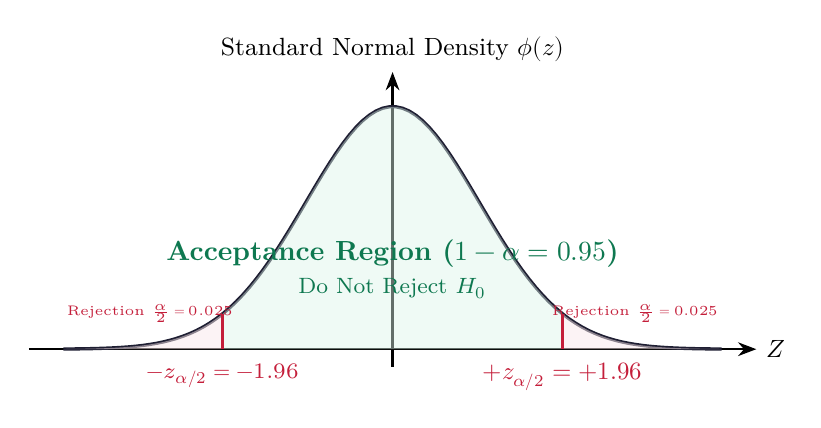
\begin{tikzpicture}[scale=1.1, every node/.style={font=\small}]
  % Axes
  \draw[-Stealth, thick] (-4.2, 0) -- (4.2, 0) node[right] {$Z$};
  \draw[-Stealth, thick] (0, -0.2) -- (0, 3.2) node[above] {Standard Normal Density $\phi(z)$};

  % Bell curve
  \draw[very thick, color=mydark, domain=-3.8:3.8, samples=100]
    plot (\x, {2.8*exp(-(\x)^2/2)});

  % Acceptance region (center)
  \fill[fill=hdrgreen, fill opacity=0.45, domain=-1.96:1.96, samples=60]
    (-1.96,0) -- plot (\x, {2.8*exp(-(\x)^2/2)}) -- (1.96,0) -- cycle;
  \node[color=mygreen, font=\bfseries] at (0, 1.1) {Acceptance Region ($1 - \alpha = 0.95$)};
  \node[color=mygreen, font=\footnotesize] at (0, 0.7) {Do Not Reject $H_0$};

  % Left critical tail (Z < -1.96)
  \fill[fill=hdrred, fill opacity=0.5, domain=-3.8:-1.96, samples=40]
    (-3.8,0) -- plot (\x, {2.8*exp(-(\x)^2/2)}) -- (-1.96,0) -- cycle;
  \draw[very thick, color=myred] (-1.96, 0) -- (-1.96, 0.41);
  \node[below, color=myred, font=\footnotesize] at (-1.96, -0.05) {$-z_{\alpha/2} = -1.96$};
  \node[above, color=myred, font=\tiny] at (-2.8, 0.2) {Rejection $\frac{\alpha}{2} = 0.025$};

  % Right critical tail (Z > +1.96)
  \fill[fill=hdrred, fill opacity=0.5, domain=1.96:3.8, samples=40]
    (1.96,0) -- plot (\x, {2.8*exp(-(\x)^2/2)}) -- (3.8,0) -- cycle;
  \draw[very thick, color=myred] (1.96, 0) -- (1.96, 0.41);
  \node[below, color=myred] at (1.96, -0.05) {$+z_{\alpha/2} = +1.96$};
  \node[above, color=myred, font=\tiny] at (2.8, 0.2) {Rejection $\frac{\alpha}{2} = 0.025$};
\end{tikzpicture}
\end{center}
\end{tcolorbox}

\subsection{Critical Values for Large Sample Tests ($Z$-Distribution)}
\par\vspace{6pt}\noindent
\begingroup
\setlength{\tabcolsep}{6pt}
\setlength{\extrarowheight}{3pt}
\begin{tabularx}{\linewidth}{|B{3.0cm}|B{3.2cm}|B{3.5cm}|Y|}
\hline
\textbf{Level of Significance ($\alpha$)} & \textbf{Two-Tailed Critical Value ($|Z| > z_{\alpha/2}$)} & \textbf{Right-Tailed Critical Value ($Z > z_\alpha$)} & \textbf{Left-Tailed Critical Value ($Z < -z_\alpha$)} \\
\hline
$\alpha = 5\% \; (0.05)$ & $z_{0.025} = 1.96$ & $z_{0.05} = 1.645$ & $-z_{0.05} = -1.645$ \\
\hline
$\alpha = 1\% \; (0.01)$ & $z_{0.005} = 2.576$ & $z_{0.01} = 2.326$ & $-z_{0.01} = -2.326$ \\
\hline
$\alpha = 10\% \; (0.10)$ & $z_{0.05} = 1.645$ & $z_{0.10} = 1.282$ & $-z_{0.10} = -1.282$ \\
\hline
\end{tabularx}
\endgroup
\vspace{12pt}

% ───────────────────────────────────────────────────────────────────────────────
\section{Large Sample Tests of Significance ($Z$-Tests, $n \ge 30$)}
% ───────────────────────────────────────────────────────────────────────────────

By the Central Limit Theorem, for sample sizes $n \ge 30$, sample statistics (proportions, means, variances) are approximately normally distributed regardless of the underlying parent population distribution. The general test statistic is:
\begin{equation}
  Z = \frac{\text{Sample Statistic} - \text{Hypothesized Parameter Value}}{\text{Standard Error of the Statistic (SE)}} \sim \mathcal{N}(0, 1)
\end{equation}

\subsection{1. Large Sample Test for a Single Proportion}
Testing whether a population proportion $P$ equals a specified value $P_0$.
\begin{tcolorbox}[formulabox, title={\textbf{Test for Single Proportion}}]
\begin{itemize}[leftmargin=*, itemsep=2pt]
  \item \textbf{Hypotheses:} $H_0: P = P_0 \quad \text{vs} \quad H_1: P \ne P_0$ (two-tailed) or $P > P_0$ (right-tailed).
  \item \textbf{Sample Proportion:} $p = \frac{x}{n}$, where $x$ is the number of successes in $n$ trials.
  \item \textbf{Standard Error under $H_0$:} $\text{SE}(p) = \sqrt{\frac{P_0 Q_0}{n}}$, where $Q_0 = 1 - P_0$.
  \item \textbf{Test Statistic:}
  \begin{equation}
    Z = \frac{p - P_0}{\sqrt{\dfrac{P_0 Q_0}{n}}}
  \end{equation}
  \item \textbf{Decision Rule:} If $|Z| > 1.96$ (at $5\%$ level), reject $H_0$.
\end{itemize}
\end{tcolorbox}

\subsection{2. Large Sample Test for Difference of Two Proportions}
Testing whether two independent populations have identical success proportions ($P_1 = P_2$).
\begin{tcolorbox}[formulabox, title={\textbf{Test for Difference of Two Proportions}}]
\begin{itemize}[leftmargin=*, itemsep=2pt]
  \item \textbf{Hypotheses:} $H_0: P_1 = P_2 \quad \text{vs} \quad H_1: P_1 \ne P_2$.
  \item \textbf{Sample Proportions:} $p_1 = \frac{x_1}{n_1}$ and $p_2 = \frac{x_2}{n_2}$.
  \item \textbf{Pooled Proportion Estimate (under $H_0$):}
  \begin{equation}
    \hat{p} = \frac{x_1 + x_2}{n_1 + n_2} = \frac{n_1 p_1 + n_2 p_2}{n_1 + n_2}, \qquad \hat{q} = 1 - \hat{p}
  \end{equation}
  \item \textbf{Test Statistic:}
  \begin{equation}
    Z = \frac{p_1 - p_2}{\sqrt{\hat{p}\hat{q}\left(\dfrac{1}{n_1} + \dfrac{1}{n_2}\right)}}
  \end{equation}
\end{itemize}
\end{tcolorbox}

\subsection{3. Large Sample Test for a Single Mean}
Testing whether a population mean $\mu$ equals a specified value $\mu_0$.
\begin{tcolorbox}[formulabox, title={\textbf{Test for Single Mean}}]
\begin{itemize}[leftmargin=*, itemsep=2pt]
  \item \textbf{Hypotheses:} $H_0: \mu = \mu_0 \quad \text{vs} \quad H_1: \mu \ne \mu_0$.
  \item \textbf{Sample Mean:} $\bar{x} = \frac{1}{n} \sum_{i=1}^n x_i$.
  \item \textbf{Test Statistic:}
  \begin{equation}
    Z = \frac{\bar{x} - \mu_0}{\sigma / \sqrt{n}}
  \end{equation}
  If the population standard deviation $\sigma$ is unknown, it is replaced by sample SD $s = \sqrt{\frac{1}{n}\sum(x_i - \bar{x})^2}$ (valid since $n \ge 30$):
  \begin{equation}
    Z = \frac{\bar{x} - \mu_0}{s / \sqrt{n}}
  \end{equation}
\end{itemize}
\end{tcolorbox}

\subsection{4. Large Sample Test for Difference of Two Means}
Testing whether two independent populations have equal means ($\mu_1 = \mu_2$).
\begin{tcolorbox}[formulabox, title={\textbf{Test for Difference of Two Means}}]
\begin{itemize}[leftmargin=*, itemsep=2pt]
  \item \textbf{Hypotheses:} $H_0: \mu_1 = \mu_2 \quad \text{vs} \quad H_1: \mu_1 \ne \mu_2$.
  \item \textbf{Test Statistic:}
  \begin{equation}
    Z = \frac{\bar{x}_1 - \bar{x}_2}{\sqrt{\dfrac{\sigma_1^2}{n_1} + \dfrac{\sigma_2^2}{n_2}}} \approx \frac{\bar{x}_1 - \bar{x}_2}{\sqrt{\dfrac{s_1^2}{n_1} + \dfrac{s_2^2}{n_2}}}
  \end{equation}
\end{itemize}
\end{tcolorbox}

\subsection{5. Large Sample Test for Difference of Standard Deviations}
Testing whether two populations have identical variability ($\sigma_1 = \sigma_2$).
\begin{tcolorbox}[formulabox, title={\textbf{Test for Difference of Two Standard Deviations}}]
For a sample of size $n$ drawn from a normal population, the sampling distribution of the sample standard deviation $s$ is asymptotically normal with mean $\sigma$ and standard error:
\begin{equation}
  \text{SE}(s) = \frac{\sigma}{\sqrt{2n}}
\end{equation}
\textbf{Test Statistic for $H_0: \sigma_1 = \sigma_2$:}
\begin{equation}
  Z = \frac{s_1 - s_2}{\sqrt{\dfrac{\sigma_1^2}{2n_1} + \dfrac{\sigma_2^2}{2n_2}}} \approx \frac{s_1 - s_2}{\sqrt{\dfrac{s_1^2}{2n_1} + \dfrac{s_2^2}{2n_2}}}
\end{equation}
\end{tcolorbox}

\newpage
% ===============================================================================
% MANDATORY QUICK REVISION PAGE
% ===============================================================================
\begin{center}
  {\large\bfseries\color{myred} Quick Revision --- Module 5}\\[1pt]
  {\small\color{mydark} Applied Statistics, Curve Fitting and Tests of Significance $|$ BS-M301}
\end{center}
\noindent{\color{myred}\rule{\linewidth}{1.0pt}}
\vspace{1pt}

\begin{tcolorbox}[formulabox, top=2pt, bottom=2pt, title={\textbf{Key Normal Equations and Large Sample $Z$-Test Formulas at a Glance}}]
\renewcommand{\arraystretch}{0.96}
\setlength{\tabcolsep}{3.5pt}
\begin{tabularx}{\linewidth}{B{3.8cm} X}
Line Normal Equations & $\sum y = n a + b \sum x, \quad \sum x y = a \sum x + b \sum x^2$ \\[0.2pt]
Parabola Normal Eqs. & $\sum y = n a + b\sum x + c\sum x^2, \; \sum xy = a\sum x + b\sum x^2 + c\sum x^3, \; \sum x^2 y = a\sum x^2 + b\sum x^3 + c\sum x^4$ \\[0.2pt]
Exponential Curve & $y = a e^{bx} \implies \ln y = \ln a + bx \implies Y = A + bx$ \\[0.2pt]
Power Curve & $y = a x^b \implies \log y = \log a + b \log x \implies Y = A + bX$ \\[0.2pt]
Single Proportion Test & $Z = \frac{p - P_0}{\sqrt{P_0 Q_0 / n}}, \quad Q_0 = 1 - P_0$ \\[0.2pt]
Two Proportions Test & $Z = \frac{p_1 - p_2}{\sqrt{\hat{p}\hat{q}(1/n_1 + 1/n_2)}}, \quad \hat{p} = \frac{n_1 p_1 + n_2 p_2}{n_1 + n_2}, \; \hat{q} = 1 - \hat{p}$ \\[0.2pt]
Single Mean Test & $Z = \frac{\bar{x} - \mu_0}{\sigma / \sqrt{n}} \approx \frac{\bar{x} - \mu_0}{s / \sqrt{n}}$ \\[0.2pt]
Two Means Test & $Z = \frac{\bar{x}_1 - \bar{x}_2}{\sqrt{\sigma_1^2/n_1 + \sigma_2^2/n_2}} \approx \frac{\bar{x}_1 - \bar{x}_2}{\sqrt{s_1^2/n_1 + s_2^2/n_2}}$ \\[0.2pt]
Standard Deviation SE & $\text{SE}(s) = \frac{\sigma}{\sqrt{2n}}, \quad Z = \frac{s_1 - s_2}{\sqrt{s_1^2/(2n_1) + s_2^2/(2n_2)}}$ \\[0.2pt]
Critical $Z$-Values & $\alpha = 5\%: |Z| = 1.96 \text{ (two-tailed)}, 1.645 \text{ (one-tailed)}; \quad \alpha = 1\%: |Z| = 2.576$ \\
\end{tabularx}
\end{tcolorbox}

\vspace{1pt}

\begin{tcolorbox}[defbox, top=2pt, bottom=2pt, title={\textbf{One-Line Definitions}}]
\begin{itemize}[leftmargin=*, itemsep=-0.5pt, topsep=0pt, parsep=0pt]
  \item \textbf{Least Squares Principle:} Criterion minimizing the sum of squared vertical residuals $\sum (y_i - f(x_i))^2$.
  \item \textbf{Normal Equations:} Set of simultaneous linear equations obtained by setting partial derivatives of error to zero.
  \item \textbf{Null Hypothesis ($H_0$):} Initial baseline claim stating no difference, no effect, or parameter equality.
  \item \textbf{Alternative Hypothesis ($H_1$):} The competing research claim adopted if sample evidence contradicts $H_0$.
  \item \textbf{Type I Error ($\alpha$):} Mistakenly rejecting a true null hypothesis (false positive; significance level).
  \item \textbf{Type II Error ($\beta$):} Incorrectly failing to reject a false null hypothesis (false negative).
  \item \textbf{Power of Test ($1 - \beta$):} Probability of correctly rejecting $H_0$ when the alternative $H_1$ is true.
  \item \textbf{Critical Region:} Subspace of test statistics leading to rejection of $H_0$ at significance level $\alpha$.
  \item \textbf{Standard Error (SE):} Standard deviation of the sampling distribution of a given sample statistic.
  \item \textbf{Pooled Proportion ($\hat{p}$):} Combined success rate $(x_1+x_2)/(n_1+n_2)$ under the null hypothesis of equality.
\end{itemize}
\end{tcolorbox}

\newpage

\begin{tcolorbox}[exambox, title={\textbf{Frequently Asked / Viva Questions (Part 1)}}]
\begin{enumerate}[topsep=0pt, label=\textbf{Q\arabic*.}, itemsep=3.2pt]
  \item \Q{State the Principle of Least Squares and explain why vertical errors are squared.}
  The principle minimizes $S = \sum e_i^2 = \sum (y_i - \hat{y}_i)^2$. Errors are squared because (1) positive and negative errors would otherwise cancel out ($\sum e_i = 0$), (2) squaring penalizes large outliers heavily, and (3) $S$ is continuously differentiable, yielding linear normal equations.

  \item \Q{How can the exponential curve $y = a b^x$ be fitted using the method of least squares?}
  Taking base-10 logarithms: $\log y = \log a + x \log b$. Defining $Y = \log y, A = \log a$, and $B = \log b$, the model becomes the linear form $Y = A + Bx$. Solving standard linear normal equations for $A$ and $B$, the parameters are recovered via $a = 10^A$ and $b = 10^B$.

  \item \Q{Distinguish between Type I Error and Type II Error in hypothesis testing.}
  Type I error ($\alpha$) occurs when a true null hypothesis $H_0$ is mistakenly rejected (false alarm). Type II error ($\beta$) occurs when a false null hypothesis is accepted (missed detection). Decreasing $\alpha$ for a fixed sample size increases $\beta$.

  \item \Q{Why can the normal distribution be used for large sample tests even if the population is non-normal?}
  By the Central Limit Theorem (CLT), the sampling distribution of the sample mean $\bar{x}$ (and sample proportions) approaches a normal distribution as sample size $n \ge 30$, irrespective of the shape of the parent population.

  \item \Q{What is the difference between a one-tailed test and a two-tailed test?}
  A two-tailed test investigates departures in either direction ($H_1: \mu \ne \mu_0$), placing critical area $\alpha/2$ in both tails. A one-tailed test investigates directional superiority or inferiority ($H_1: \mu > \mu_0$ or $\mu < \mu_0$), concentrating the entire critical area $\alpha$ in one tail.

  \item \Q{State the standard error of the sample standard deviation for a normal population.}
  For large samples drawn from a normal population, $\text{SE}(s) = \frac{\sigma}{\sqrt{2n}}$. It is used to test significance of variance differences across industrial production lines.

  \item \Q{Why do we pool the proportions $\hat{p} = \frac{n_1 p_1 + n_2 p_2}{n_1 + n_2}$ in the two-proportion test?}
  Under the null hypothesis $H_0: P_1 = P_2 = P$, both samples originate from a single population with common proportion $P$. Pooling gives the minimum-variance unbiased estimator of this common parameter.
\end{enumerate}
\end{tcolorbox}

\newpage

\begin{tcolorbox}[exambox, top=3pt, bottom=3pt, title={\textbf{Frequently Asked / Viva Questions (Part 2)}}]
\begin{enumerate}[topsep=0pt, label=\textbf{Q\arabic*.}, itemsep=1.8pt, start=8]
  \item \Q{What decision is made if the calculated test statistic is $Z_{\text{cal}} = 2.15$ at $5\%$ significance level?}
  For a two-tailed test at $\alpha = 5\%$, the critical boundary is $Z_{\text{crit}} = 1.96$. Since $|Z_{\text{cal}}| = 2.15 > 1.96$, the sample statistic falls in the critical rejection region. We reject the null hypothesis $H_0$ and conclude the observed difference is statistically significant.

  \item \Q{How does shifting the origin simplify fitting a parabola $y = a + bx + cx^2$?}
  If $x$ values are symmetrically spaced, shifting the origin to the center makes $\sum u = 0$ and $\sum u^3 = 0$. The normal equations decouple into $b = \sum uy / \sum u^2$, while $a$ and $c$ decouple from $b$ into an elementary $2 \times 2$ system, dramatically reducing computational effort.

  \item \Q{What is the Level of Significance ($\alpha$) and how is it related to the confidence level?}
  The level of significance $\alpha$ is the maximum tolerable probability of committing a Type I error. It is related to the confidence level $C$ by $C = (1 - \alpha) \times 100\%$. For example, an $\alpha = 0.05$ level of significance corresponds to a $95\%$ confidence level.
\end{enumerate}
\end{tcolorbox}

\vspace{2pt}

\begin{tcolorbox}[tikzbox, top=3pt, bottom=3pt, title={\textbf{Summary Matrix: Comprehensive Decision Table of Large Sample Significance Tests}}]
\par\vspace{1pt}\noindent
\begingroup
\setlength{\tabcolsep}{3.5pt}
\setlength{\extrarowheight}{1.0pt}
\renewcommand{\arraystretch}{1.12}
\begin{tabularx}{\linewidth}{|B{2.5cm}|B{3.5cm}|B{3.2cm}|Y|}
\hline
\textbf{Test Type} & \textbf{Null Hypothesis ($H_0$)} & \textbf{Standard Error (SE)} & \textbf{Test Statistic ($Z_{\text{cal}}$)} \\
\hline
Single Proportion & $H_0: P = P_0$ & $\sqrt{\frac{P_0 Q_0}{n}}$ & $Z = \frac{p - P_0}{\sqrt{P_0 Q_0 / n}}$ \\
\hline
Two Proportions & $H_0: P_1 = P_2$ & $\sqrt{\hat{p}\hat{q}\left(\frac{1}{n_1} + \frac{1}{n_2}\right)}$ & $Z = \frac{p_1 - p_2}{\sqrt{\hat{p}\hat{q}(1/n_1 + 1/n_2)}}, \quad \hat{p} = \frac{n_1 p_1 + n_2 p_2}{n_1 + n_2}$ \\
\hline
Single Mean & $H_0: \mu = \mu_0$ & $\frac{\sigma}{\sqrt{n}} \approx \frac{s}{\sqrt{n}}$ & $Z = \frac{\bar{x} - \mu_0}{s / \sqrt{n}}$ \\
\hline
Two Means & $H_0: \mu_1 = \mu_2$ & $\sqrt{\frac{s_1^2}{n_1} + \frac{s_2^2}{n_2}}$ & $Z = \frac{\bar{x}_1 - \bar{x}_2}{\sqrt{s_1^2/n_1 + s_2^2/n_2}}$ \\
\hline
Two Std. Deviations & $H_0: \sigma_1 = \sigma_2$ & $\sqrt{\frac{s_1^2}{2n_1} + \frac{s_2^2}{2n_2}}$ & $Z = \frac{s_1 - s_2}{\sqrt{s_1^2/(2n_1) + s_2^2/(2n_2)}}$ \\
\hline
\end{tabularx}
\endgroup
\end{tcolorbox}


% -- Module 6 -----------------------------------------------------------------
\modulestart{6}{Introduction to Small Sample Theory}

\section{Introduction to Small Sample Theory}
% ===============================================================================

\begin{tcolorbox}[defbox, title={\textbf{Definition: Small Samples vs. Large Samples}}]
In statistical hypothesis testing, a sample is designated as a \textbf{small sample} if its sample size $n < 30$.
\begin{itemize}[leftmargin=12pt, itemsep=2pt]
  \item \textbf{Large Samples ($n \ge 30$):} By the Central Limit Theorem (CLT), the sampling distribution of sample means approaches normality regardless of the parent distribution. The sample standard deviation $s$ closely approximates the population standard deviation $\sigma$, justifying the use of the standard normal $Z$-test.
  \item \textbf{Small Samples ($n < 30$):} The CLT cannot be invoked. The parent population \textbf{must be assumed normally distributed}. Furthermore, replacing $\sigma$ with the sample variance $s^2 = \frac{1}{n-1}\sum (x_i - \bar{x})^2$ introduces substantial additional sampling fluctuations, yielding distributions with heavier tails than $N(0, 1)$.
\end{itemize}
Hence, small sample inference relies on the \textbf{exact sampling distributions}:
\begin{enumerate}[leftmargin=16pt, itemsep=1pt]
  \item \textbf{Student's $t$-distribution} (W.~S.~Gosset, 1908): For inference on population means and correlation coefficients when $\sigma$ is unknown.
  \item \textbf{Snedecor's $F$-distribution} (G.~W.~Snedecor \& R.~A.~Fisher): For testing the ratio of two independent population variances.
  \item \textbf{Chi-square ($\chi^2$) distribution} (Karl Pearson, 1900): For tests of goodness of fit and independence of attributes in contingency tables.
\end{enumerate}
\end{tcolorbox}

\begin{tcolorbox}[formulabox, title={\textbf{Degrees of Freedom ($\nu$ or d.f.)}}]
The \textbf{degrees of freedom} ($\nu$) of a test statistic represents the number of unconstrained, freely variable observations available in the calculation:
\begin{equation}
  \nu = n - k
\end{equation}
where $n$ is the total number of sample observations and $k$ is the number of linear constraints or sample-derived parameters estimated to compute the statistic (e.g., estimating $\mu$ by $\bar{x}$ consumes 1 d.f., so $\nu = n - 1$).
\end{tcolorbox}

% ===============================================================================
\section{Student's \texorpdfstring{$t$}{t}-Distribution}
% ===============================================================================

\subsection{Definition and Derivation}

\begin{tcolorbox}[defbox, title={\textbf{Mathematical Definition of Student's $t$-Variable}}]
Let $Z \sim N(0, 1)$ be a standard normal random variable, and let $Y \sim \chi^2(\nu)$ be an independent Chi-square random variable with $\nu$ degrees of freedom. The ratio:
\begin{equation}
  T = \frac{Z}{\sqrt{\dfrac{Y}{\nu}}}
\end{equation}
follows \textbf{Student's $t$-distribution} with $\nu$ degrees of freedom, written $T \sim t(\nu)$.
\end{tcolorbox}

\subsection{Probability Density Function and Properties}

The probability density function (PDF) of $T \sim t(\nu)$ is:
\begin{equation}
  f(t) = \frac{1}{\sqrt{\nu}\,\mathrm{B}\left(\dfrac{1}{2}, \dfrac{\nu}{2}\right)}\left(1 + \frac{t^2}{\nu}\right)^{-\frac{\nu+1}{2}}, \quad -\infty < t < \infty
\end{equation}
where $\mathrm{B}\left(\frac{1}{2}, \frac{\nu}{2}\right) = \frac{\sqrt{\pi}\,\Gamma(\nu/2)}{\Gamma((\nu+1)/2)}$ is the Beta function.

\begin{tcolorbox}[formulabox, title={\textbf{Key Properties of Student's $t$-Distribution}}]
\begin{enumerate}[leftmargin=14pt, itemsep=2pt]
  \item \textbf{Symmetry:} The curve is bell-shaped and symmetric about $t = 0$. All odd central moments are zero:
  \begin{equation}
    \mu_{2k+1} = E[T^{2k+1}] = 0 \quad (\text{for } \nu > 2k+1)
  \end{equation}
  \item \textbf{Mean:} $\mu_1' = E[T] = 0$ (valid for $\nu > 1$).
  \item \textbf{Variance:} $\mathrm{Var}(T) = \mu_2 = \dfrac{\nu}{\nu - 2}$ (valid for $\nu > 2$). Note that $\mathrm{Var}(T) > 1$.
  \item \textbf{Kurtosis (Heavy Tails):} The distribution is leptokurtic ($\beta_2 > 3$). For $\nu > 4$:
  \begin{equation}
    \beta_2 = \frac{\mu_4}{\mu_2^2} = 3 + \frac{6}{\nu - 4} > 3
  \end{equation}
  \item \textbf{Limiting Form (Asymptotic Normality):} As $\nu \to \infty$, the $t$-distribution converges to the standard normal distribution:
  \begin{equation}
    \lim_{\nu \to \infty} \left(1 + \frac{t^2}{\nu}\right)^{-\frac{\nu+1}{2}} = e^{-t^2/2} \implies t(\nu) \xrightarrow{d} N(0, 1)
  \end{equation}
\end{enumerate}
\end{tcolorbox}

\begin{tcolorbox}[tikzbox, title={\textbf{TikZ Illustration: Comparison of Student's $t$ vs. Standard Normal $N(0, 1)$}}]
\centering
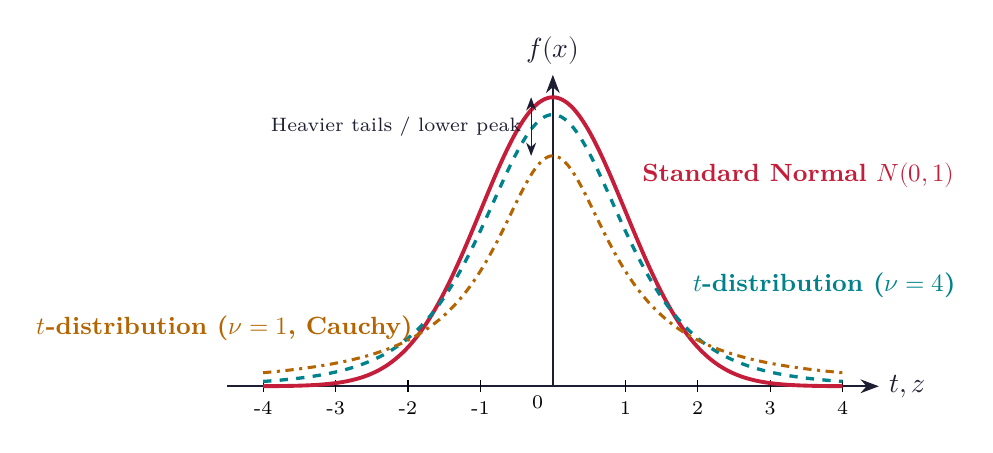
\begin{tikzpicture}[scale=0.92]
  \draw[arrow] (-4.5, 0) -- (4.5, 0) node[right] {$t, z$};
  \draw[arrow] (0, 0) -- (0, 4.3) node[above] {$f(x)$};

  \foreach \x in {-4, -3, -2, -1, 1, 2, 3, 4}
    \draw (\x, 0.08) -- (\x, -0.08) node[below, font=\scriptsize] {\x};
  \node[below left, font=\scriptsize] at (0, 0) {$0$};

  % Normal curve N(0,1): f(0) = 0.3989 -> 3.99 cm
  \draw[line width=1.4pt, color=myred, domain=-4:4, samples=100, smooth]
    plot (\x, {3.989 * exp(-\x*\x / 2)});
  \node[color=myred, font=\small\bfseries, above right] at (1.1, 2.6) {Standard Normal $N(0, 1)$};

  % Student's t, nu = 4: f(0) = 0.375 -> 3.75 cm
  \draw[line width=1.2pt, color=myteal, dashed, domain=-4:4, samples=100, smooth]
    plot (\x, {3.75 * (1 + \x*\x / 4)^(-2.5)});
  \node[color=myteal, font=\small\bfseries, right] at (1.8, 1.4) {$t$-distribution ($\nu = 4$)};

  % Student's t, nu = 1 (Cauchy): f(0) = 1/pi -> 3.18 cm
  \draw[line width=1.1pt, color=myamber, dashdotted, domain=-4:4, samples=100, smooth]
    plot (\x, {3.183 / (1 + \x*\x)});
  \node[color=myamber, font=\small\bfseries, left] at (-1.8, 0.8) {$t$-distribution ($\nu = 1$, Cauchy)};

  % Heavier tails annotation
  \draw[<->, >=Stealth, color=mydark] (-0.3, 3.18) -- (-0.3, 3.99) node[midway, left, font=\scriptsize] {Heavier tails / lower peak};
\end{tikzpicture}
\end{tcolorbox}

\newpage
% ===============================================================================
\section{Student's \texorpdfstring{$t$}{t}-Tests of Significance}
% ===============================================================================

\subsection{Test for Single Mean}

\begin{tcolorbox}[formulabox, title={\textbf{Test 1: Single Mean $t$-Test Formulation}}]
Let $x_1, x_2, \ldots, x_n$ be a random sample of size $n < 30$ drawn from a normal population $N(\mu, \sigma^2)$ where $\sigma$ is unknown. We test:
\begin{equation}
  H_0: \mu = \mu_0 \quad \text{vs.} \quad H_1: \mu \ne \mu_0 \quad (\text{or one-sided } \mu > \mu_0, \mu < \mu_0)
\end{equation}
The test statistic is:
\begin{equation}
  t = \frac{\bar{x} - \mu_0}{s / \sqrt{n}}
\end{equation}
where $\bar{x} = \frac{1}{n}\sum_{i=1}^n x_i$ and the \textbf{unbiased sample variance} is:
\begin{equation}
  s^2 = \frac{1}{n - 1} \sum_{i=1}^n (x_i - \bar{x})^2 = \frac{1}{n - 1}\left(\sum_{i=1}^n x_i^2 - \frac{(\sum x_i)^2}{n}\right)
\end{equation}
Under $H_0$, $t \sim t(\nu)$ with degrees of freedom $\nu = n - 1$.

\textbf{Decision Rule (Two-tailed at significance level $\alpha$):}
\begin{itemize}[leftmargin=12pt, itemsep=2pt]
  \item Reject $H_0$ if $|t_{\text{cal}}| > t_{\alpha/2, n-1}$.
  \item Fail to reject $H_0$ if $|t_{\text{cal}}| \le t_{\alpha/2, n-1}$.
\end{itemize}
\textbf{$100(1-\alpha)\%$ Confidence Interval for $\mu$:}
\begin{equation}
  \bar{x} - t_{\alpha/2, n-1} \frac{s}{\sqrt{n}} \le \mu \le \bar{x} + t_{\alpha/2, n-1} \frac{s}{\sqrt{n}}
\end{equation}
\end{tcolorbox}

\begin{tcolorbox}[examplebox, title={\textbf{Worked Example: Single Mean $t$-Test}}]
A manufacturer claims that the mean lifetime of an electronic component is 1000 hours. A random sample of 9 components yields a sample mean of 980 hours with a sample standard deviation $s = 30$ hours. Test at the 5\% level whether the true mean lifetime is significantly less than 1000 hours ($t_{0.05, 8} = 1.860$).

\textbf{Solution:}
\begin{enumerate}[leftmargin=14pt, itemsep=2pt]
  \item \textbf{Hypotheses:} $H_0: \mu = 1000$ vs. $H_1: \mu < 1000$ (one-tailed left-sided test).
  \item \textbf{Parameters:} $n = 9$, $\bar{x} = 980$, $s = 30$, $\mu_0 = 1000$.
  \item \textbf{Test Statistic:}
  \begin{equation*}
    t_{\text{cal}} = \frac{\bar{x} - \mu_0}{s / \sqrt{n}} = \frac{980 - 1000}{30 / \sqrt{9}} = \frac{-20}{10} = -2.00
  \end{equation*}
  \item \textbf{Critical Value:} For left-tailed test at $\alpha = 0.05$ with $\nu = 8$: $t_{\text{crit}} = -1.860$.
  \item \textbf{Conclusion:} Since $t_{\text{cal}} = -2.00 < -1.860$, $t_{\text{cal}}$ falls in the critical rejection region. We reject $H_0$ and conclude that the mean lifetime is significantly less than 1000 hours.
\end{enumerate}
\end{tcolorbox}

\subsection{Test for Difference of Two Means (Independent Samples)}

\begin{tcolorbox}[formulabox, title={\textbf{Test 2: Two-Sample Independent $t$-Test with Pooled Variance}}]
Let two independent samples of sizes $n_1$ and $n_2$ be drawn from normal populations $N(\mu_1, \sigma^2)$ and $N(\mu_2, \sigma^2)$ with \textbf{equal unknown variance} ($\sigma_1^2 = \sigma_2^2 = \sigma^2$). We test:
\begin{equation}
  H_0: \mu_1 = \mu_2 \quad \text{vs.} \quad H_1: \mu_1 \ne \mu_2
\end{equation}
The \textbf{pooled unbiased variance} $s_p^2$ combining both samples is:
\begin{equation}
  s_p^2 = \frac{\sum_{i=1}^{n_1} (x_{1i} - \bar{x}_1)^2 + \sum_{j=1}^{n_2} (x_{2j} - \bar{x}_2)^2}{n_1 + n_2 - 2} = \frac{(n_1 - 1)s_1^2 + (n_2 - 1)s_2^2}{n_1 + n_2 - 2}
\end{equation}
The test statistic is:
\begin{equation}
  t = \frac{\bar{x}_1 - \bar{x}_2}{s_p \sqrt{\dfrac{1}{n_1} + \dfrac{1}{n_2}}}
\end{equation}
Under $H_0$, $t \sim t(\nu)$ with degrees of freedom $\nu = n_1 + n_2 - 2$.
\end{tcolorbox}

\subsection{Paired \texorpdfstring{$t$}{t}-Test for Dependent Samples}

\begin{tcolorbox}[defbox, title={\textbf{Test 3: Paired $t$-Test Principle}}]
When observations in two samples are drawn in matched pairs (e.g., measurements taken on the \textbf{same physical circuit before and after} temperature cycling), the two groups are statistically dependent. We eliminate inter-subject variability by evaluating individual differences:
\begin{equation}
  d_i = x_i - y_i, \quad i = 1, 2, \ldots, n
\end{equation}
Under the null hypothesis of no treatment effect ($H_0: \mu_d = 0$):
\begin{equation}
  t = \frac{\bar{d} - 0}{s_d / \sqrt{n}}
\end{equation}
where:
\begin{equation}
  \bar{d} = \frac{1}{n}\sum_{i=1}^n d_i, \qquad s_d^2 = \frac{1}{n - 1}\sum_{i=1}^n (d_i - \bar{d})^2 = \frac{\sum d_i^2 - \dfrac{(\sum d_i)^2}{n}}{n - 1}
\end{equation}
The statistic follows Student's $t$-distribution with $\nu = n - 1$ degrees of freedom.
\end{tcolorbox}

\subsection{Test for Significance of Correlation Coefficient}

\begin{tcolorbox}[formulabox, title={\textbf{Test 4: Significance of Correlation Coefficient}}]
Let $r$ be the Pearson sample correlation coefficient calculated from $n$ pairs of observations drawn from a bivariate normal population. To test:
\begin{equation}
  H_0: \rho = 0 \quad (\text{variables are uncorrelated}) \quad \text{vs.} \quad H_1: \rho \ne 0
\end{equation}
The test statistic is:
\begin{equation}
  t = \frac{r \sqrt{n - 2}}{\sqrt{1 - r^2}}
\end{equation}
Under $H_0$, $t \sim t(\nu)$ with degrees of freedom $\nu = n - 2$. Reject $H_0$ if $|t_{\text{cal}}| > t_{\alpha/2, n-2}$.
\end{tcolorbox}

\newpage
% ===============================================================================
\section{Snedecor's \texorpdfstring{$F$}{F}-Distribution and Test for Ratio of Variances}
% ===============================================================================

\subsection{Definition and Properties}

\begin{tcolorbox}[defbox, title={\textbf{Definition of Snedecor's $F$-Distribution}}]
Let $U \sim \chi^2(\nu_1)$ and $V \sim \chi^2(\nu_2)$ be two independent Chi-square random variables with $\nu_1$ and $\nu_2$ degrees of freedom, respectively. The ratio:
\begin{equation}
  F = \frac{U / \nu_1}{V / \nu_2}
\end{equation}
follows \textbf{Snedecor's $F$-distribution} with $(\nu_1, \nu_2)$ degrees of freedom, denoted $F \sim F(\nu_1, \nu_2)$.
\end{tcolorbox}

\begin{tcolorbox}[formulabox, title={\textbf{Properties of the $F$-Distribution}}]
\begin{enumerate}[leftmargin=14pt, itemsep=2pt]
  \item \textbf{Support and Shape:} $F \in (0, \infty)$. The distribution is positively skewed (right-skewed) and unimodal.
  \item \textbf{Mean:} $E[F] = \dfrac{\nu_2}{\nu_2 - 2}$ (for $\nu_2 > 2$, independent of $\nu_1$).
  \item \textbf{Variance:} $\mathrm{Var}(F) = \dfrac{2\nu_2^2(\nu_1 + \nu_2 - 2)}{\nu_1(\nu_2 - 2)^2(\nu_2 - 4)}$ (for $\nu_2 > 4$).
  \item \textbf{Reciprocal Property:} If $F \sim F(\nu_1, \nu_2)$, then $\dfrac{1}{F} \sim F(\nu_2, \nu_1)$. Hence:
  \begin{equation}
    F_{1-\alpha, \nu_1, \nu_2} = \frac{1}{F_{\alpha, \nu_2, \nu_1}}
  \end{equation}
  \item \textbf{Relation to $t$ and $\chi^2$:}
  \begin{equation}
    F_{1, \nu} = t_\nu^2, \qquad \lim_{\nu_2 \to \infty} \nu_1 F_{\nu_1, \nu_2} = \chi^2(\nu_1)
  \end{equation}
\end{enumerate}
\end{tcolorbox}

\subsection{\texorpdfstring{$F$}{F}-Test for Equality of Two Population Variances}

\begin{tcolorbox}[formulabox, title={\textbf{$F$-Test Procedure for $\sigma_1^2 = \sigma_2^2$}}]
Let two independent random samples of sizes $n_1$ and $n_2$ be drawn from normal populations $N(\mu_1, \sigma_1^2)$ and $N(\mu_2, \sigma_2^2)$. We test:
\begin{equation}
  H_0: \sigma_1^2 = \sigma_2^2 \quad \text{vs.} \quad H_1: \sigma_1^2 \ne \sigma_2^2 \quad (\text{or } \sigma_1^2 > \sigma_2^2)
\end{equation}
Compute the unbiased sample variances:
\begin{equation}
  s_1^2 = \frac{1}{n_1 - 1}\sum_{i=1}^{n_1} (x_{1i} - \bar{x}_1)^2, \qquad s_2^2 = \frac{1}{n_2 - 1}\sum_{j=1}^{n_2} (x_{2j} - \bar{x}_2)^2
\end{equation}
By convention, we place the larger sample variance in the numerator:
\begin{equation}
  F_{\text{cal}} = \frac{s_1^2}{s_2^2} \ge 1 \quad (\text{assuming } s_1^2 \ge s_2^2)
\end{equation}
with degrees of freedom $\nu_1 = n_1 - 1$ (numerator) and $\nu_2 = n_2 - 1$ (denominator). Reject $H_0$ at level $\alpha$ if $F_{\text{cal}} > F_{\alpha/2, \nu_1, \nu_2}$.
\end{tcolorbox}

\begin{tcolorbox}[tikzbox, title={\textbf{TikZ Schematic: Right-Skewed $F$-Distribution with Critical Region}}]
\centering
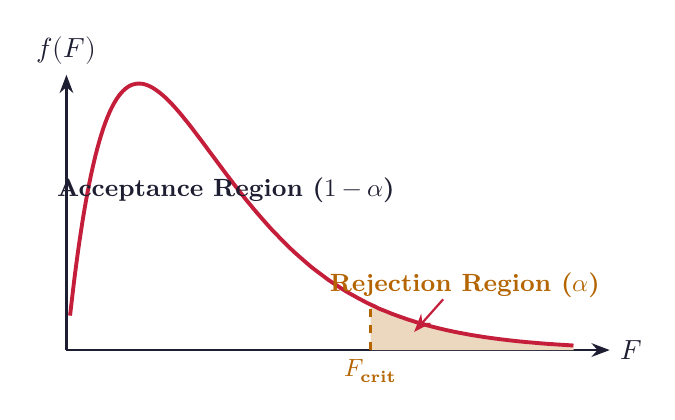
\begin{tikzpicture}[scale=0.92]
  \draw[arrow] (0, 0) -- (7.5, 0) node[right] {$F$};
  \draw[arrow] (0, 0) -- (0, 3.8) node[above] {$f(F)$};

  % Shaded rejection region
  \fill[myamber!25] plot[domain=4.2:7, samples=50] (\x, {10 * \x * exp(-\x)}) -- (7, 0) -- (4.2, 0) -- cycle;

  % F curve
  \draw[line width=1.4pt, color=myred, domain=0.05:7, samples=120, smooth]
    plot (\x, {10 * \x * exp(-\x)});

  % Critical line
  \draw[dashed, line width=1.2pt, color=myamber] (4.2, 0) -- (4.2, 0.63);
  \node[below, color=myamber, font=\small\bfseries] at (4.2, 0) {$F_{\text{crit}}$};

  % Annotations
  \node[font=\small\bfseries, color=mydark] at (2.2, 2.2) {Acceptance Region ($1 - \alpha$)};
  \node[font=\small\bfseries, color=myamber] at (5.5, 0.9) {Rejection Region ($\alpha$)};
  \draw[redarrow] (5.2, 0.7) -- (4.8, 0.25);
\end{tikzpicture}
\end{tcolorbox}

\newpage
% ===============================================================================
\section{Chi-Square (\texorpdfstring{$\chi^2$}{Chi-Square}) Distribution}
% ===============================================================================

\subsection{Definition and Properties}

\begin{tcolorbox}[defbox, title={\textbf{Definition of Chi-Square Distribution}}]
If $Z_1, Z_2, \ldots, Z_\nu$ are $\nu$ independent standard normal random variables ($Z_i \sim N(0, 1)$), the sum of their squares:
\begin{equation}
  X = \sum_{i=1}^\nu Z_i^2
\end{equation}
follows a \textbf{Chi-square distribution} with $\nu$ degrees of freedom, denoted $X \sim \chi^2(\nu)$.
\end{tcolorbox}

\begin{tcolorbox}[formulabox, title={\textbf{Mathematical Properties of $\chi^2(\nu)$}}]
\begin{enumerate}[leftmargin=14pt, itemsep=2pt]
  \item \textbf{Probability Density Function:}
  \begin{equation}
    f(x) = \frac{1}{2^{\nu/2}\Gamma(\nu/2)}\, x^{\frac{\nu}{2} - 1} e^{-x/2}, \quad x \ge 0
  \end{equation}
  \item \textbf{Mean and Variance:}
  \begin{equation}
    E[X] = \nu, \qquad \mathrm{Var}(X) = 2\nu
  \end{equation}
  \item \textbf{Moment Generating Function (MGF):}
  \begin{equation}
    M_X(t) = (1 - 2t)^{-\nu/2}, \quad \text{for } t < \frac{1}{2}
  \end{equation}
  \item \textbf{Additive (Reproductive) Property:} If $X_1 \sim \chi^2(\nu_1)$ and $X_2 \sim \chi^2(\nu_2)$ are independent:
  \begin{equation}
    X_1 + X_2 \sim \chi^2(\nu_1 + \nu_2)
  \end{equation}
  \item \textbf{Limiting Form:} For large $\nu$ ($\nu > 30$), $\sqrt{2\chi^2} - \sqrt{2\nu - 1} \approx N(0, 1)$.
\end{enumerate}
\end{tcolorbox}

\begin{tcolorbox}[tikzbox, title={\textbf{TikZ Plot: Chi-Square Curves for Degrees of Freedom $\nu = 1, 3, 5, 10$}}]
\centering
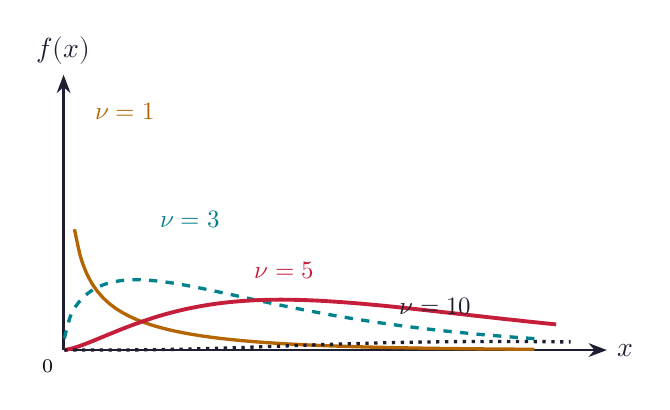
\begin{tikzpicture}[scale=0.92]
  \draw[arrow] (0, 0) -- (7.5, 0) node[right] {$x$};
  \draw[arrow] (0, 0) -- (0, 3.8) node[above] {$f(x)$};

  \node[below left, font=\scriptsize] at (0, 0) {$0$};

  % nu = 1 (L-shaped)
  \draw[line width=1.2pt, color=myamber, domain=0.15:6.5, samples=80, smooth]
    plot (\x, {0.7 * \x^(-0.5) * exp(-\x / 2)});
  \node[color=myamber, font=\small\bfseries, right] at (0.3, 3.3) {$\nu = 1$};

  % nu = 3 (starts at 0)
  \draw[line width=1.2pt, color=myteal, dashed, domain=0.01:6.5, samples=80, smooth]
    plot (\x, {1.6 * \x^(0.5) * exp(-\x / 2)});
  \node[color=myteal, font=\small\bfseries, right] at (1.2, 1.8) {$\nu = 3$};

  % nu = 5
  \draw[line width=1.4pt, color=myred, domain=0.01:6.8, samples=80, smooth]
    plot (\x, {0.6 * \x^(1.5) * exp(-\x / 2)});
  \node[color=myred, font=\small\bfseries, right] at (2.5, 1.1) {$\nu = 5$};

  % nu = 10
  \draw[line width=1.2pt, color=mydark, dotted, domain=0.01:7, samples=80, smooth]
    plot (\x, {0.005 * \x^4 * exp(-\x / 1.5)});
  \node[color=mydark, font=\small\bfseries, right] at (4.5, 0.6) {$\nu = 10$};
\end{tikzpicture}
\end{tcolorbox}

\newpage
% ===============================================================================
\section{Chi-Square Test of Goodness of Fit}
% ===============================================================================

\subsection{Principle and Pearson's Test Statistic}

\begin{tcolorbox}[defbox, title={\textbf{Pearson's Chi-Square Goodness of Fit}}]
The goodness of fit test evaluates whether an observed frequency distribution conforms to a theoretical probability distribution (such as Binomial, Poisson, or Normal). Let:
\begin{itemize}[leftmargin=12pt, itemsep=2pt]
  \item $O_i$ = Observed frequency in the $i$-th class ($i = 1, 2, \ldots, k$).
  \item $E_i$ = Expected frequency under theoretical model, with $\sum_{i=1}^k E_i = \sum_{i=1}^k O_i = N$.
\end{itemize}
Karl Pearson proved that the test statistic:
\begin{equation}
  \chi^2 = \sum_{i=1}^k \frac{(O_i - E_i)^2}{E_i} = \sum_{i=1}^k \frac{O_i^2}{E_i} - N
\end{equation}
asymptotically follows a Chi-square distribution with $\nu$ degrees of freedom:
\begin{equation}
  \nu = k - 1 - m
\end{equation}
where $k$ is the number of classes after pooling, and $m$ is the number of independent population parameters estimated from the sample data.
\end{tcolorbox}

\begin{tcolorbox}[formulabox, title={\textbf{Conditions for Validity of $\chi^2$ Test}}]
To ensure accurate approximation of discrete multinomial probabilities by continuous $\chi^2$:
\begin{enumerate}[leftmargin=14pt, itemsep=2pt]
  \item \textbf{Total Sample Size:} $N = \sum O_i \ge 50$.
  \item \textbf{Minimum Expected Frequency:} Each $E_i \ge 5$. If any $E_i < 5$, it must be \textbf{pooled (combined)} with adjacent classes, reducing $k$.
  \item \textbf{Independent Observations:} Sampling units must be mutually independent.
  \item \textbf{Linear Constraint:} $\sum O_i = \sum E_i = N$, which consumes 1 degree of freedom.
\end{enumerate}
\end{tcolorbox}

\begin{tcolorbox}[examplebox, title={\textbf{Worked Example: Chi-Square Test of Goodness of Fit}}]
A die is rolled 120 times, yielding the following face frequencies: 15, 23, 18, 16, 26, 22. Test at the 5\% level whether the die is fair ($\chi^2_{0.05, 5} = 11.07$).

\textbf{Solution:}
\begin{enumerate}[leftmargin=14pt, itemsep=2pt]
  \item \textbf{Hypotheses:} $H_0$: The die is fair ($p_i = 1/6$) vs. $H_1$: The die is biased.
  \item \textbf{Expected Frequencies:} $E_i = 120 \times \frac{1}{6} = 20$ for all $i = 1, \ldots, 6$. All $E_i \ge 5$.
  \item \textbf{Computation Table:}
\end{enumerate}
\par\vspace{2pt}\noindent
\begin{tabularx}{\linewidth}{*{5}{>{\small\centering\arraybackslash}X}}
\toprule
\textbf{Face ($i$)} & \textbf{Observed ($O_i$)} & \textbf{Expected ($E_i$)} & $O_i - E_i$ & $(O_i - E_i)^2 / E_i$ \\
\midrule
1 & 15 & 20 & $-5$ & $25 / 20 = 1.25$ \\
2 & 23 & 20 & $+3$ & $9 / 20 = 0.45$ \\
3 & 18 & 20 & $-2$ & $4 / 20 = 0.20$ \\
4 & 16 & 20 & $-4$ & $16 / 20 = 0.80$ \\
5 & 26 & 20 & $+6$ & $36 / 20 = 1.80$ \\
6 & 22 & 20 & $+2$ & $4 / 20 = 0.20$ \\
\midrule
\textbf{Total} & \textbf{120} & \textbf{120} & \textbf{0} & $\mathbf{\chi^2_{\text{cal}} = 4.70}$ \\
\bottomrule
\end{tabularx}
\par\vspace{4pt}
\textbf{Decision:} With $\nu = 6 - 1 = 5$ d.f., $\chi^2_{\text{crit}} = 11.07$. Since $\chi^2_{\text{cal}} = 4.70 < 11.07$, we fail to reject $H_0$. The die is consistent with being unbiased.
\end{tcolorbox}

\newpage
% ===============================================================================
\section{Chi-Square Test for Independence of Attributes}
% ===============================================================================

\subsection{\texorpdfstring{$r \times c$}{r x c} Contingency Tables}

\begin{tcolorbox}[defbox, title={\textbf{Contingency Table and Expected Cell Frequency}}]
When $N$ observations are classified simultaneously across two qualitative attributes $A$ (with $r$ levels $A_1, \ldots, A_r$) and $B$ (with $c$ levels $B_1, \ldots, B_c$), the frequencies form an $r \times c$ contingency table.

\textbf{Null Hypothesis:} $H_0$: Attributes $A$ and $B$ are independent.

Under $H_0$, $P(A_i \cap B_j) = P(A_i)P(B_j)$, yielding the \textbf{expected cell frequency} $E_{ij}$:
\begin{equation}
  E_{ij} = N \times \left(\frac{R_i}{N}\right) \times \left(\frac{C_j}{N}\right) = \frac{R_i \times C_j}{N}
\end{equation}
where $R_i$ is the $i$-th row total, $C_j$ is the $j$-th column total, and $N$ is the grand total.
The test statistic is:
\begin{equation}
  \chi^2 = \sum_{i=1}^r \sum_{j=1}^c \frac{(O_{ij} - E_{ij})^2}{E_{ij}}
\end{equation}
with degrees of freedom:
\begin{equation}
  \nu = (r - 1)(c - 1)
\end{equation}
\end{tcolorbox}

\subsection{\texorpdfstring{$2 \times 2$}{2 x 2} Contingency Table and Yates' Continuity Correction}

\begin{tcolorbox}[formulabox, title={\textbf{$2 \times 2$ Contingency Table Formula}}]
For a $2 \times 2$ contingency table with counts:
\par\vspace{2pt}\noindent
\begin{center}
\begin{tabular}{c c c c}
\toprule
 & $B_1$ & $B_2$ & \textbf{Total} \\
\midrule
$A_1$ & $a$ & $b$ & $a + b$ \\
$A_2$ & $c$ & $d$ & $c + d$ \\
\midrule
\textbf{Total} & $a + c$ & $b + d$ & $N = a + b + c + d$ \\
\bottomrule
\end{tabular}
\end{center}
\par\vspace{2pt}
The standard chi-square statistic ($\nu = (2-1)(2-1) = 1$) simplifies algebraically to:
\begin{equation}
  \chi^2 = \frac{N (ad - bc)^2}{(a + b)(c + d)(a + c)(b + d)}
\end{equation}

\textbf{Yates' Correction for Continuity:}
Because $\chi^2$ is continuous while counts $a, b, c, d$ are discrete integers, Frank Yates introduced a correction when $\nu = 1$ and any cell frequency is small ($< 5$):
\begin{equation}
  \chi_{\text{corr}}^2 = \frac{N \left(|ad - bc| - \dfrac{N}{2}\right)^2}{(a + b)(c + d)(a + c)(b + d)}
\end{equation}
This continuity correction reduces $\chi^2_{\text{cal}}$, preventing inflated Type I error rates.
\end{tcolorbox}

\newpage
% ===============================================================================
% QUICK REVISION SPREAD (MANDATORY 3-PAGE SPREAD)
% ===============================================================================

% ─── QUICK REVISION PAGE 1 OF 3: Formulas & Definitions ────────────────────────
\begin{center}
  {\large\bfseries\color{myred} Quick Revision --- Module 6}\\[1pt]
  {\small\color{mydark} Small Samples: $t$-Test, $F$-Test, and Chi-Square Distribution $|$ BS-M301}
\end{center}
\noindent{\color{myred}\rule{\linewidth}{1.0pt}}
\vspace{1pt}

\begin{tcolorbox}[formulabox, top=2pt, bottom=2pt, title={\textbf{Key Small Sample and Chi-Square Formulas at a Glance}}]
\renewcommand{\arraystretch}{0.94}
\setlength{\tabcolsep}{3.5pt}
\begin{tabularx}{\linewidth}{B{3.8cm} X}
Single Mean $t$-Test & $t = \frac{\bar{x} - \mu_0}{s / \sqrt{n}}, \quad s^2 = \frac{1}{n-1}\sum (x_i - \bar{x})^2, \quad \nu = n - 1$ \\[0.2pt]
Two-Sample Mean $t$-Test & $t = \frac{\bar{x}_1 - \bar{x}_2}{s_p\sqrt{1/n_1 + 1/n_2}}, \quad s_p^2 = \frac{(n_1-1)s_1^2 + (n_2-1)s_2^2}{n_1+n_2-2}, \quad \nu = n_1 + n_2 - 2$ \\[0.2pt]
Paired $t$-Test & $t = \frac{\bar{d}}{s_d / \sqrt{n}}, \quad d_i = x_i - y_i, \quad s_d^2 = \frac{1}{n-1}\sum (d_i - \bar{d})^2, \quad \nu = n - 1$ \\[0.2pt]
Correlation $t$-Test & $t = \frac{r\sqrt{n-2}}{\sqrt{1-r^2}}, \quad \nu = n - 2$ \\[0.2pt]
Fisher's $F$-Statistic & $F = \frac{s_1^2}{s_2^2} \ge 1, \quad \nu_1 = n_1 - 1, \quad \nu_2 = n_2 - 1$ \\[0.2pt]
$\chi^2$ Goodness of Fit & $\chi^2 = \sum_{i=1}^k \frac{(O_i - E_i)^2}{E_i}, \quad \nu = k - 1 - m$ \\[0.2pt]
$2 \times 2$ Contingency $\chi^2$ & $\chi^2 = \frac{N(ad - bc)^2}{(a+b)(c+d)(a+c)(b+d)}, \quad \nu = 1$ \\[0.2pt]
Yates' Correction & $\chi_{\text{corr}}^2 = \frac{N\left(|ad - bc| - N/2\right)^2}{(a+b)(c+d)(a+c)(b+d)}$ \\
\end{tabularx}
\end{tcolorbox}

\vspace{-2pt}

\begin{tcolorbox}[defbox, top=2pt, bottom=2pt, title={\textbf{One-Line Definitions}}]
\small
\begin{itemize}[leftmargin=11pt, itemsep=-0.6pt, topsep=0pt]
  \item \textbf{Small Sample:} A statistical sample with size $n < 30$, requiring exact distributions ($t, F, \chi^2$) rather than the standard normal $Z$-test.
  \item \textbf{Degrees of Freedom ($\nu$):} The number of unconstrained, freely variable observations used in evaluating a sample statistic ($\nu = n - k$).
  \item \textbf{Student's $t$-Distribution:} The exact distribution of the ratio of a standard normal variable to the square root of an independent $\chi^2$ variable divided by its d.f.
  \item \textbf{Pooled Variance ($s_p^2$):} The weighted average of two independent sample variances used in two-sample $t$-tests under equal population variances.
  \item \textbf{Paired $t$-Test:} A test applied to dependent matched pairs where differences $d_i = x_i - y_i$ eliminate extraneous subject variability.
  \item \textbf{Snedecor's $F$-Distribution:} The distribution of the ratio of two independent chi-square variables, each divided by its d.f. ($s_1^2 / s_2^2$).
  \item \textbf{Chi-Square ($\chi^2$) Distribution:} The distribution formed by the sum of squares of $\nu$ independent standard normal random variables.
  \item \textbf{Goodness of Fit:} A statistical test measuring whether an empirical sample frequency distribution adheres to a theoretical distribution.
  \item \textbf{Contingency Table:} A grid matrix displaying the bivariate joint frequency distribution of two qualitative attributes.
  \item \textbf{Yates' Correction:} A continuity correction subtracting $N/2$ from $|ad - bc|$ in $2 \times 2$ tables to account for discrete counts in continuous $\chi^2$.
\end{itemize}
\end{tcolorbox}

\newpage
% ─── QUICK REVISION PAGE 2 OF 3: Viva Q&A Part 1 ───────────────────────────────
\begin{tcolorbox}[exambox, title={\textbf{Frequently Asked / Viva Questions (Part 1)}}]
\small
\begin{enumerate}[leftmargin=14pt, itemsep=3pt]
\item \Q{Q1. Why can we not use the standard normal $Z$-test for small samples ($n < 30$)?}
For $n < 30$, the Central Limit Theorem cannot guarantee normality of the sampling distribution unless the parent population is normal. Furthermore, substituting the sample variance $s^2$ for the unknown $\sigma^2$ introduces substantial additional sampling variability, making the tails of the distribution much heavier than $N(0, 1)$. Gosset's $t$-distribution accounts precisely for this extra variability.

\item \Q{Q2. What are the key assumptions underlying the two-sample independent $t$-test?}
The assumptions are: (1) both parent populations are normally distributed, (2) the two samples are selected randomly and independently, and (3) the two population variances are equal ($\sigma_1^2 = \sigma_2^2 = \sigma^2$, known as homoscedasticity). Equality of variances is checked using an $F$-test.

\item \Q{Q3. When should a paired $t$-test be used instead of an independent two-sample $t$-test?}
A paired $t$-test must be used when the two sets of observations are intrinsically dependent, such as measurements on the same physical subjects before and after a treatment, or twin studies. It isolates the treatment effect by converting paired data into single differences $d_i = x_i - y_i$, thereby eliminating between-subject biological or physical variance.

\item \Q{Q4. State the relation between Student's $t$, Snedecor's $F$, and Chi-square $\chi^2$ distributions.}
Key interrelations include:
\begin{itemize}[leftmargin=12pt, itemsep=1pt]
  \item The square of a $t$-variable with $\nu$ d.f.\ is an $F$-variable with $(1, \nu)$ d.f.: $t_\nu^2 = F_{1, \nu}$.
  \item As the denominator degrees of freedom $\nu_2 \to \infty$, $\nu_1 F_{\nu_1, \nu_2} \to \chi^2(\nu_1)$.
  \item As degrees of freedom $\nu \to \infty$, Student's $t(\nu) \to N(0, 1)$.
\end{itemize}

\item \Q{Q5. Why is the larger sample variance always placed in the numerator in an $F$-test?}
By convention, setting $F = s_1^2 / s_2^2$ with $s_1^2 \ge s_2^2$ ensures $F \ge 1$. This allows the use of standard upper-tail $F$-distribution critical value tables without needing to invert lower-tail critical values ($F_{1-\alpha} = 1 / F_\alpha$).

\item \Q{Q6. What are the fundamental validity conditions for Karl Pearson's Chi-square test?}
The conditions are: (1) total sample size $N = \sum O_i \ge 50$, (2) each theoretical expected frequency $E_i \ge 5$ (if $E_i < 5$, adjacent cells must be pooled), (3) individual observations are drawn randomly and independently, and (4) $\sum O_i = \sum E_i = N$.

\item \Q{Q7. How are degrees of freedom calculated in an $r \times c$ contingency table?}
The degrees of freedom are $\nu = (r - 1)(c - 1)$. This arises because the marginal row totals impose $r$ constraints and the column totals impose $c$ constraints, with one common grand total constraint $N$, leaving $(r-1)(c-1)$ independently assignable cells.
\end{enumerate}
\end{tcolorbox}

\newpage
% ─── QUICK REVISION PAGE 3 OF 3: Viva Q&A Part 2 & Summary Comparison Matrix ───
\begin{tcolorbox}[exambox, title={\textbf{Frequently Asked / Viva Questions (Part 2)}}]
\small
\begin{enumerate}[leftmargin=14pt, itemsep=3pt]
\setcounter{enumi}{7}
\item \Q{Q8. What is Yates' correction for continuity and when is it mandatory?}
Yates' correction adjusts the discrete cell counts in a $2 \times 2$ table to match the continuous theoretical $\chi^2$ density by subtracting $N/2$ from the absolute difference $|ad - bc|$. It is mandatory when $\nu = 1$ and any cell frequency is less than 5 ($E_{ij} < 5$), preventing spurious rejections of $H_0$.

\item \Q{Q9. How do you test whether an observed sample correlation coefficient $r = 0.6$ from $n = 18$ pairs is statistically significant?}
We test $H_0: \rho = 0$ using $t = \frac{r\sqrt{n-2}}{\sqrt{1-r^2}} = \frac{0.6\sqrt{16}}{\sqrt{1 - 0.36}} = \frac{0.6 \times 4}{0.8} = 3.00$. With $\nu = 18 - 2 = 16$ d.f., the critical value at $\alpha = 0.05$ is $t_{0.025, 16} = 2.12$. Since $|t_{\text{cal}}| = 3.00 > 2.12$, the correlation is statistically significant.

\item \Q{Q10. What does a non-significant result in a $\chi^2$ goodness-of-fit test signify?}
When $\chi^2_{\text{cal}} \le \chi^2_{\text{crit}}$, we fail to reject $H_0$. This indicates that the observed sampling discrepancies from theoretical frequencies are small enough to be attributed purely to chance, confirming the theoretical model fits the empirical data well.
\end{enumerate}
\end{tcolorbox}

\vspace{-2pt}

\begin{tcolorbox}[tikzbox, top=2pt, bottom=2pt, title={\textbf{Summary Matrix: Comparison of Small Sample Tests ($t$, $F$, $\chi^2$)}}]
\renewcommand{\arraystretch}{0.96}
\setlength{\tabcolsep}{3.5pt}
\par\vspace{1pt}\noindent
\begin{tabularx}{\linewidth}{B{2.3cm} B{2.5cm} Y >{\small\centering\arraybackslash}X}
\toprule
\textbf{Test} & \textbf{Objective} & \textbf{Test Statistic \& Parameters} & \textbf{d.f. ($\nu$)} \\
\midrule
Single Mean $t$ & Test $H_0: \mu = \mu_0$ ($\sigma$ unknown) & $t = \dfrac{\bar{x} - \mu_0}{s / \sqrt{n}}, \quad s^2 = \dfrac{\sum(x_i - \bar{x})^2}{n - 1}$ & $n - 1$ \\
Two-Sample $t$ & Compare two means ($\sigma_1 = \sigma_2$) & $t = \dfrac{\bar{x}_1 - \bar{x}_2}{s_p\sqrt{1/n_1 + 1/n_2}}$, pooled $s_p^2$ & $n_1 + n_2 - 2$ \\
Paired $t$ & Before vs. After on same units & $t = \dfrac{\bar{d}}{s_d / \sqrt{n}}$, differences $d_i = x_i - y_i$ & $n - 1$ \\
Correlation $t$ & Test $H_0: \rho = 0$ & $t = \dfrac{r\sqrt{n-2}}{\sqrt{1 - r^2}}$ & $n - 2$ \\
Fisher's $F$ & Compare $\sigma_1^2$ vs $\sigma_2^2$ & $F = \dfrac{s_1^2}{s_2^2}$ ($s_1^2 \ge s_2^2$) & $(n_1 - 1, n_2 - 1)$ \\
Pearson's $\chi^2$ & Goodness of Fit & $\chi^2 = \sum \dfrac{(O_i - E_i)^2}{E_i}$ & $k - 1 - m$ \\
Contingency $\chi^2$ & Independence of attributes & $\chi^2 = \sum \sum \dfrac{(O_{ij} - E_{ij})^2}{E_{ij}}$ or $2 \times 2$ Yates & $(r - 1)(c - 1)$ \\
\bottomrule
\end{tabularx}
\end{tcolorbox}


\end{document}
